%!TEX program = xelatex
\documentclass[12pt,openany]{report}

% Load the unified preamble (all packages, fonts, macros)

%%%%%%%%%%%%%%%%%%%%%%%%%%%%%%%%%%%%%%%%%%%%%%%%%%%%%%%%%%%%%%%%%%%%%%%
%           VIETNAMESE LATEX THESIS PREAMBLE - XELATEX OPTIMIZED
%%%%%%%%%%%%%%%%%%%%%%%%%%%%%%%%%%%%%%%%%%%%%%%%%%%%%%%%%%%%%%%%%%%%%%%

% --- XeLaTeX required ---
\usepackage{fontspec}
% --- Polyglossia for Vietnamese and English --
\usepackage{polyglossia}
\setmainlanguage{vietnamese}
\setotherlanguage{english}

%%%%%%%%%%%%%%%%%%%%%%%%%%%%%%%%%%%%%%%%%%%%%%%%%%%%%%%%%%%%%%%%%%%%%%%%
%                        FONT CONFIGURATION
%%%%%%%%%%%%%%%%%%%%%%%%%%%%%%%%%%%%%%%%%%%%%%%%%%%%%%%%%%%%%%%%%%%%%%%%
\setmainfont{Liberation Serif}[
    BoldFont = Liberation Serif Bold,
    ItalicFont = Liberation Serif Italic,
    BoldItalicFont = Liberation Serif Bold Italic
]
\setsansfont{Liberation Sans}[
    BoldFont = Liberation Sans Bold,
    ItalicFont = Liberation Sans Italic,
    BoldItalicFont = Liberation Sans Bold Italic
]
\setmonofont{Liberation Mono}[Scale=0.9]

\newfontfamily{\vietfont}{Liberation Serif}[Scale=MatchLowercase]

% Unicode math
\usepackage{unicode-math}
\setmathfont{Latin Modern Math}

% Microtype (XeLaTeX compatible)
\usepackage[protrusion=true, expansion=false]{microtype}
\microtypesetup{kerning=false, spacing=true}

%%%%%%%%%%%%%%%%%%%%%%%%%%%%%%%%%%%%%%%%%%%%%%%%%%%%%%%%%%%%%%%%%%%%%%%%
%                    ADDITIONAL PACKAGES
%%%%%%%%%%%%%%%%%%%%%%%%%%%%%%%%%%%%%%%%%%%%%%%%%%%%%%%%%%%%%%%%%%%%%%%%

\usepackage{xcolor}
\usepackage{minted} % minted với cache để tránh cần shell-escape mỗi lần
\usepackage{graphicx}
\graphicspath{{figures/}{chapters/ch2_background/}{chapters/ch3_methodology/}}
\usepackage{calc}
\usepackage{url}
\usepackage{amsmath}
\usepackage{caption}
\usepackage{subcaption}
\captionsetup{justification=centering, labelfont=bf}
\captionsetup[subfigure]{justification=centering}

% Màu cho minted
\definecolor{darkblue}{RGB}{0,0,139}
\definecolor{lightgray}{gray}{0.95}

% Cấu hình minted
\setminted{
    frame=single,
    linenos=true,
    numbersep=10pt,
    bgcolor=lightgray,
    fontsize=\small,
    breaklines=true,
    tabsize=4,
    xleftmargin=10pt,
    escapeinside=||
}

% Bibliography
\usepackage[backend=biber,style=ieee]{biblatex}
\addbibresource{references.bib}

%%%%%%%%%%%%%%%%%%%%%%%%%%%%%%%%%%%%%%%%%%%%%%%%%%%%%%%%%%%%%%%%%%%%%%%%
%                    CUSTOM MACROS FOR THESIS
%%%%%%%%%%%%%%%%%%%%%%%%%%%%%%%%%%%%%%%%%%%%%%%%%%%%%%%%%%%%%%%%%%%%%%%%
\newcommand{\TENLUANVAN}{Hệ thống phát hiện và cảnh báo té ngã thời gian thực tích hợp cảm biến, xử lý ảnh và định vị}
\newcommand{\THESISNAME}{Real-time fall detection and alert system integrating sensors, image processing, and positioning}
\newcommand{\TENTACGIA}{Tran Hao}
\newcommand{\MASOSV}{173401}
\newcommand{\KHOA}{Điện - Điện tử}
\newcommand{\BOMON}{Viễn thông}
\newcommand{\TENNGUOIHUONGDAN}{PSG.TS Ha Hoang Kha}
\newcommand{\NAMBAOVE}{2025}
\newcommand{\DEPARTMENT}{\KHOA}
\newcommand{\TENTACGIAFACULTY}{\TENTACGIA}
\newcommand{\MSSV}{\MASOSV}
\newcommand{\TENCANBO}{\TENNGUOIHUONGDAN}

%%%%%%%%%%%%%%%%%%%%%%%%%%%%%%%%%%%%%%%%%%%%%%%%%%%%%%%%%%%%%%%%%%%%%%%%
%                        PAGE & LAYOUT SETTINGS
%%%%%%%%%%%%%%%%%%%%%%%%%%%%%%%%%%%%%%%%%%%%%%%%%%%%%%%%%%%%%%%%%%%%%%%%
\usepackage{geometry}
\geometry{
    top=2.5cm,
    bottom=2.5cm,
    left=3.0cm,
    right=2.0cm,
    headheight=18pt,
    headsep=12pt,
    footskip=20pt
}

\usepackage{setspace}
\onehalfspacing
\usepackage{indentfirst}
\setlength{\parindent}{1.2em}
\setlength{\parskip}{0pt}
\tolerance=2000
\emergencystretch=0.5em
\hyphenpenalty=5000
\exhyphenpenalty=5000

%%%%%%%%%%%%%%%%%%%%%%%%%%%%%%%%%%%%%%%%%%%%%%%%%%%%%%%%%%%%%%%%%%%%%%%%
%                     HEADER, FOOTER & TITLES
%%%%%%%%%%%%%%%%%%%%%%%%%%%%%%%%%%%%%%%%%%%%%%%%%%%%%%%%%%%%%%%%%%%%%%%%
\usepackage{titlesec}
\usepackage{fancyhdr}
\pagestyle{fancy}
\fancyhf{}
\fancyhead[L]{\nouppercase{\leftmark}}
\fancyfoot[C]{\thepage}
\renewcommand{\headrulewidth}{0.4pt}
\renewcommand{\footrulewidth}{0pt}
\renewcommand{\chaptermark}[1]{\markboth{\chaptername\ \thechapter.\ #1}{}}

% Hyperref (load last)
\usepackage{hyperref}
\hypersetup{
    colorlinks=true,
    linkcolor=darkblue,
    urlcolor=darkblue,
    citecolor=darkblue,
    pdfauthor={\TENTACGIA},
    pdftitle={\TENLUANVAN}
}


\begin{document}

% --- FRONTMATTER ---
\pagenumbering{roman}
\pagestyle{empty}

% Title page

\begin{titlepage}
\thispagestyle{empty}
\begin{center}
    \setlength{\fboxrule}{2pt}   % Độ dày viền
    \setlength{\fboxsep}{20pt}   % Khoảng cách từ viền đến nội dung
    
    \fcolorbox{darkblue}{white}{%
        \begin{minipage}{0.93\textwidth}
            \vspace*{0.8cm}
            \centering
            
            \textbf{ĐẠI HỌC QUỐC GIA TP. HỒ CHÍ MINH} \\[0.2cm]
            \textbf{TRƯỜNG ĐẠI HỌC BÁCH KHOA} \\[0.2cm]
            \textbf{KHOA ĐIỆN - ĐIỆN TỬ} \\[0.2cm]
            
            \textbf{\rule{0.25\textwidth}{0.4pt} \, \ding{118} \, \rule{0.25\textwidth}{0.4pt}} \\[0.8cm]
            
            
\includegraphics[width=0.25\textwidth]{figures/logo_hcmut.png} \\[0.8cm]
            
            {\Large \textbf{BÁO CÁO LUẬN VĂN}} \\[1cm]
            
            \parbox{0.9\textwidth}{\centering
                \textbf{ĐỀ TÀI: Hệ thống phát hiện và cảnh báo té ngã thời gian thực tích hợp cảm biến,\\ xử lý ảnh và định vị} \\[0.3cm]
                \textit{\THESISNAME}
            } \\[1cm]
            
            \begin{tabular}{rl}
                \textbf{GVHD:} & \TENNGUOIHUONGDAN \\[0.3cm]
                \textbf{SVTH:} & \TENTACGIA \\[0.3cm]
                \textbf{MSSV:} & \MSSV
            \end{tabular} \\[1cm]
            
            \textbf{TP. HỒ CHÍ MINH, THÁNG 07/2025}
            
            \vspace*{0.8cm}
        \end{minipage}
    }
\end{center}
\end{titlepage}


% Abstract
\cleardoublepage
\chapter*{TÓM TẮT}
\addcontentsline{toc}{chapter}{TÓM TẮT}

Luận văn này trình bày việc thiết kế và triển khai một hệ thống phát hiện té ngã đa phương thức dành cho người cao tuổi và bệnh nhân cần giám sát liên tục. Hệ thống sử dụng ESP32 kết hợp với cảm biến quán tính MPU6050 để thu thập dữ liệu chuyển động, đồng thời phân tích luồng video thời gian thực bằng các thuật toán thị giác máy tính, nâng cao độ chính xác trong việc nhận diện các sự kiện té ngã.

Dữ liệu cảm biến và cảnh báo được mã hóa dưới định dạng JSON và truyền thông qua giao thức MQTT, cho phép trao đổi thông tin thời gian thực giữa thiết bị nhúng và máy chủ. Python trên máy chủ Linux xử lý dữ liệu, đánh giá mức độ cảnh báo và điều khiển Asterisk PBX để thực hiện các hành động viễn thông tự động như gọi điện thoại, gửi tin nhắn SMS và chia sẻ hình ảnh sự kiện qua ứng dụng Telegram.

Hệ thống được thiết kế theo kiến trúc mô-đun, dễ mở rộng và tối ưu chi phí, đồng thời đảm bảo tính đáng tin cậy, bảo mật dữ liệu và khả năng hoạt động ổn định trong môi trường gia đình hoặc cơ sở chăm sóc y tế. Kết quả nghiên cứu cung cấp một giải pháp toàn diện, kết hợp nhúng IoT, viễn thông và xử lý dữ liệu thông minh, góp phần nâng cao chất lượng giám sát và phản ứng kịp thời với các sự kiện té ngã.



% Acknowledgements
\cleardoublepage
\thispagestyle{empty}
\begin{center}
    \vspace*{1.5cm}
    \textbf{\fontsize{16}{19}\selectfont LỜI CẢM ƠN}
    \vspace{0.8cm}
\end{center}

\noindent
\setlength{\parindent}{1.5cm}
\setlength{\parskip}{6pt}
\fontsize{12}{14}\selectfont  

Trước hết, tôi xin bày tỏ lòng biết ơn chân thành và sâu sắc đến \textbf{PGS.TS. Hà Hoàng Kha} người đã tận tâm hướng dẫn và đồng hành cùng tôi trong suốt quá trình thực hiện đồ án này. Thầy không chỉ tận tình chỉ bảo từng bước trong nghiên cứu đề tài, mà còn thường xuyên đốc thúc tôi hoàn thành công việc đúng tiến độ và hướng dẫn để báo cáo được trình bày một cách logic, khoa học. Tôi trân trọng những lời nhắc nhở sâu sắc của thầy về thái độ học tập và làm việc. Thầy khuyến khích việc tiếp cận vấn đề một cách thực chất, tìm tòi và học hỏi để kiến thức thực sự trở thành của mình, thay vì hoàn thành một cách hình thức. Sự hỗ trợ quý báu này đã giúp tôi tích lũy nhiều kinh nghiệm, hoàn thiện kiến thức chuyên môn và nâng cao kỹ năng nghiên cứu một cách chuyên nghiệp hơn.

Tôi cũng xin bày tỏ lòng biết ơn đến các thầy cô trong \textbf{Bộ môn Viễn Thông, Khoa Điện – Điện tử, Trường Đại học Bách khoa – Đại học Quốc gia TP. Hồ Chí Minh} những người đã trang bị cho tôi nền tảng kiến thức vững chắc và tạo điều kiện thuận lợi để tôi tiếp cận, phát triển chuyên môn một cách toàn diện. Tôi trân trọng cảm ơn Nhà trường và Bộ môn đã tạo môi trường học tập tích cực và hiệu quả, với cơ sở vật chất, tài liệu học tập và các hoạt động hỗ trợ nghiên cứu.

Đặc biệt, tôi xin gửi lời cảm ơn sâu sắc đến \textbf{gia đình} điểm tựa tinh thần vững chắc nhất của tôi. Sự động viên, tin tưởng và những hy sinh thầm lặng của gia đình chính là nguồn động lực to lớn giúp tôi kiên trì và hoàn thành luận văn này.

Cuối cùng, tôi xin chân thành cảm ơn tất cả những người đã giúp đỡ và hỗ trợ tôi trong quá trình học tập và hoàn thiện luận văn. Mỗi sự hỗ trợ dù lớn hay nhỏ đều góp phần quan trọng tạo nên kết quả ngày hôm nay.

\vspace{0.8cm}
\begin{flushright}
    \begin{minipage}{0.5\textwidth}
        \centering
        \textit{Tp. Hồ Chí Minh, ngày....tháng.....năm 2025} \\
        \vspace{0.8cm}
        \textbf{Sinh viên} \\
        \vspace{0.3cm}
        \textbf{Trần Đức Hảo}
    \end{minipage}
\end{flushright}

\vfill
\clearpage


% Faculty / Department info (thường sẽ được đặt ở đầu cùng)
\cleardoublepage

\thispagestyle{empty}
\setstretch{0.85} % giãn dòng vừa phải

% ------------------- HEADER: TÊN TRƯỜNG + SỐ + KHOA/BỘ MÔN -------------------
\begin{center}
\begin{minipage}[t]{0.48\textwidth}
\centering
\textbf{\small ĐẠI HỌC QUỐC GIA TP.HCM} \\
\textbf{\small TRƯỜNG ĐẠI HỌC BÁCH KHOA} \\
\vspace{0.2cm}
\textbf{\small ------oOo------} \\ % Dòng phân cách
\vspace{0.2cm}
Số: \underline{\hspace{3cm}} /BK-ĐPT \\[0.2cm]
\textbf{\small Khoa: \DEPARTMENT} \\
\textbf{\small Bộ Môn: Viễn Thông}
\end{minipage}
\hfill
\begin{minipage}[t]{0.48\textwidth}
\centering
\textbf{\small CỘNG HOÀ XÃ HỘI CHỦ NGHĨA} \\
\textbf{\small VIỆT NAM} \\
\textbf{\small Độc lập -- Tự do -- Hạnh phúc} \\
\vspace{0.2cm}
\textbf{\small ------oOo------} % Dòng phân cách
\end{minipage}
\end{center}

\vspace{0.6cm}

% ------------------- TIÊU ĐỀ TRANG -------------------
\begin{center}
\textbf{\large NHIỆM VỤ LUẬN VĂN}
\end{center}

\vspace{0.5cm}

% ------------------- THÔNG TIN SINH VIÊN -------------------
\noindent
1. Họ và tên: \TENTACGIA \hspace{2cm} MSSV: \MSSV

\vspace{0.2cm}
\noindent 2. Ngành: Điện tử - Viễn Thông

\vspace{0.2cm}
\noindent 3. Đề tài: \TENLUANVAN

\vspace{0.2cm}
\noindent 4. Nhiệm vụ: .................................................. 

\vspace{0.4cm}
\noindent 5. Ngày giao nhiệm vụ luận văn: .............................................. 

\vspace{0.2cm}
\noindent 6. Ngày hoàn thành nhiệm vụ: ..............................................

\vspace{0.2cm}
\noindent 7. Họ và tên người hướng dẫn: \TENCANBO

\vspace{0.4cm}
\noindent Nội dung và yêu cầu luận văn đã được thông qua Bộ Môn.

\vspace{0.3cm}
\noindent \hfill \textit{Tp. Hồ Chí Minh, ngày ...... tháng ...... năm 2025}

% ------------------- CHỮ KÝ -------------------
\vspace{0.5cm}
\begin{center}
\begin{minipage}[t]{0.48\textwidth}
\centering
\textbf{CHỦ NHIỆM BỘ MÔN} \\[2.5cm]
\textbf{\small (Ký và ghi rõ họ tên)}
\end{minipage}
\hfill
\begin{minipage}[t]{0.48\textwidth}
\centering
\textbf{NGƯỜI HƯỚNG DẪN CHÍNH} \\[2.5cm]
\textbf{\small (Ký và ghi rõ họ tên)}
\end{minipage}
\end{center}


% ------------------- PHẦN DÀNH CHO KHOA, BỘ MÔN -------------------
\vspace{0.3cm}
\noindent
\begin{minipage}[t]{\textwidth}
\textbf{PHẦN DÀNH CHO KHOA, BỘ MÔN:}\\
\vspace{0.2cm}
\small
Người duyệt (chấm sơ bộ): \dotfill \\[0.2cm]
Ngày ký: \dotfill \\[0.2cm]
Điểm đánh giá: \dotfill \\[0.2cm]
Nhận xét: \dotfill \\[0.2cm]
\phantom{Nhận xét: } \dotfill \\[0.2cm]
Lưu tại bộ môn: \dotfill
\end{minipage}


% Set the page style for the rest of the frontmatter
\pagestyle{fancy}

% Table of contents
\cleardoublepage
\phantomsection
\addcontentsline{toc}{chapter}{Mục lục}
\tableofcontents

% List of figures
\cleardoublepage
\phantomsection
\addcontentsline{toc}{chapter}{Danh mục hình ảnh}
\listoffigures

% List of tables
\cleardoublepage
\phantomsection
\addcontentsline{toc}{chapter}{Danh mục bảng biểu}
\listoftables

% --- MAINMATTER ---
\cleardoublepage
\pagenumbering{arabic}
\pagestyle{fancy}

% Chapters (ensure each file exists in chapters/ folder)

\chapter{Tổng quan vấn đề té ngã, tình hình nghiên cứu trong và ngoài nước}

\section{Tổng quan vấn đề té ngã và hệ thống phát hiện té ngã}

Té ngã là một trong những nguyên nhân hàng đầu gây chấn thương nghiêm trọng và tử vong không chủ ý, đặc biệt ở nhóm dân số cao tuổi. Theo số liệu của Tổ chức Y tế Thế giới (\textbf{WHO}), trung bình mỗi năm có khoảng 646.000 người tử vong do té ngã, trong đó hơn 80\% xảy ra ở các quốc gia thu nhập trung bình và thấp. Người cao tuổi (trên 65 tuổi) là nhóm có nguy cơ cao nhất, với tỷ lệ té ngã trên 30\% mỗi năm và tăng lên tới 50\% ở nhóm trên 80 tuổi. \textbf{Mức độ nghiêm trọng của vấn đề được minh họa chi tiết trong Hình 1.1.}

\begin{figure}[h]
    \centering
    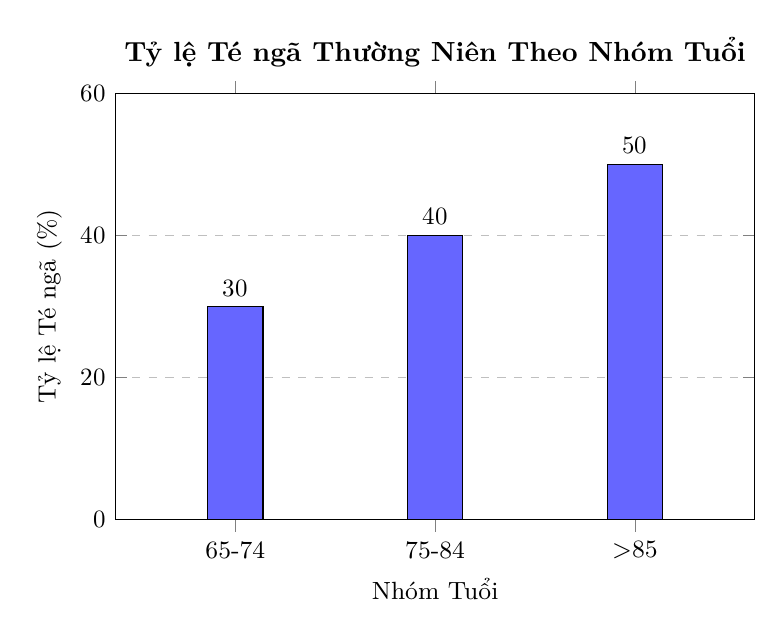
\begin{tikzpicture}
        \begin{axis}[
            ybar,
            ymin=0,
            ymax=60, % Đặt max y để biểu đồ cân đối
            ylabel={Tỷ lệ Té ngã (\%)},
            xlabel={Nhóm Tuổi},
            xtick=data,
            symbolic x coords={65-74, 75-84, >85},
            bar width=20pt,
            nodes near coords,
            nodes near coords style={font=\small, color=black, /pgf/number format/.cd, fixed, precision=0},
            title={Tỷ lệ Té ngã Thường Niên Theo Nhóm Tuổi},
            enlarge x limits=0.3,
            height=7cm,
            width=0.8\textwidth,
            ymajorgrids=true,
            grid style=dashed,
            tick label style={font=\small},
            title style={font=\bfseries, align=center},
            xlabel style={font=\small},
            ylabel style={font=\small}
        ]
        \addplot[fill=blue!60] coordinates {
            (65-74, 30)
            (75-84, 40)
            (>85, 50)
        };
        \end{axis}
    \end{tikzpicture}
    \caption{Tỷ lệ té ngã thường niên ở người cao tuổi (Dữ liệu thống kê).}
    \label{fig:ti_le_nga}
\end{figure}
Riêng tại Việt Nam, tình trạng già hóa dân số đang diễn ra nhanh chóng; số liệu từ Tổng cục Thống kê cho thấy tỷ lệ người trên 60 tuổi chiếm khoảng 12\% dân số vào năm 2020 và dự báo sẽ tăng gấp đôi vào năm 2049. Điều này đặt ra áp lực đáng kể cho hệ thống y tế, đặc biệt trong công tác chăm sóc và giám sát người cao tuổi tại nhà hoặc tại các cơ sở chăm sóc chuyên biệt.

Té ngã không chỉ gây ra tổn thương thể chất như gãy xương hông, chấn thương sọ não hay tổn thương cột sống, mà còn ảnh hưởng nghiêm trọng đến tâm lý người bệnh. Một khi đã từng té ngã, người cao tuổi thường phát triển hội chứng sợ té, dẫn tới giảm hoạt động, suy yếu chức năng vận động và kéo theo sự suy giảm chất lượng cuộc sống toàn diện. Nghiêm trọng hơn, nếu té ngã xảy ra khi nạn nhân ở một mình và không có khả năng cầu cứu, hậu quả có thể rất nghiêm trọng. Thời gian nằm bất động kéo dài có thể gây ra các biến chứng như hạ thân nhiệt, mất nước, hoại tử do loét tì đè, hoặc thậm chí tử vong do không được cấp cứu kịp thời.

Trong bối cảnh đó, các \textbf{hệ thống phát hiện và cảnh báo té ngã tự động} đang trở thành một xu hướng tất yếu trong lĩnh vực y tế công nghệ cao. Các hệ thống này có khả năng phát hiện hành vi té ngã dựa trên phân tích tín hiệu từ nhiều nguồn cảm biến khác nhau như gia tốc kế, con quay hồi chuyển (\textbf{gyroscope}), cảm biến áp suất, hoặc \textbf{phân tích hình ảnh thời gian thực}. Khi được thiết kế đúng cách, các hệ thống này không chỉ nhận diện chính xác sự cố té ngã mà còn có khả năng gửi cảnh báo nhanh chóng đến người thân, nhân viên y tế hoặc các cơ quan cứu trợ. Đặc biệt, việc tích hợp định vị \textbf{GPS} giúp cung cấp vị trí chính xác của nạn nhân, tối ưu hoá thời gian phản ứng và can thiệp. Việc xây dựng và tối ưu hóa các hệ thống này chính là trọng tâm của luận văn này, và sẽ được đặt trong bối cảnh nghiên cứu toàn cầu ở phần tiếp theo.

% Preparing the LaTeX document with necessary packages
\section{Tình hình nghiên cứu trong và ngoài nước}

% Subsection for research context
\subsection{Tổng quan bối cảnh nghiên cứu}
Sự gia tăng dân số cao tuổi toàn cầu đã đặt ra những thách thức lớn về y tế và an toàn cá nhân, đặc biệt liên quan đến tai nạn té ngã. Theo Tổ chức Y tế Thế giới (WHO), té ngã là nguyên nhân hàng đầu gây thương tích không cố ý ở người cao tuổi, chiếm khoảng 684.000 ca tử vong mỗi năm và hàng triệu ca chấn thương không gây tử vong khác~\cite{who2021}. Thực trạng này đã thúc đẩy cộng đồng nghiên cứu toàn cầu tập trung phát triển các hệ thống phát hiện té ngã tự động, với mục tiêu giảm thiểu thương tích, cải thiện chất lượng chăm sóc và khả năng phản ứng kịp thời.

% Listing main approaches to fall detection
Các phương pháp phát hiện té ngã hiện nay có thể được phân loại chính thành ba hướng:  
\begin{enumerate}
    \item \textbf{Phương pháp dựa trên thị giác máy tính (Vision-based)}: Sử dụng camera để thu thập dữ liệu hình ảnh/video, áp dụng các thuật toán nhận diện tư thế người và phân tích động học để xác định tình huống té ngã.  
    \item \textbf{Phương pháp dựa trên cảm biến đeo trên người (Wearable sensor-based)}: Sử dụng các cảm biến quán tính như IMU, gia tốc kế, con quay hồi chuyển gắn trên thiết bị đeo tay hoặc dây đeo để theo dõi chuyển động và phát hiện té ngã.  
    \item \textbf{Phương pháp kết hợp đa phương thức (Multi-modal)}: Tích hợp dữ liệu từ nhiều nguồn, ví dụ kết hợp camera và cảm biến IMU, nhằm tận dụng ưu điểm của từng phương pháp và giảm tỷ lệ cảnh báo sai.
\end{enumerate}

% Subsection for international research
\subsection{Nghiên cứu quốc tế}
Trên thế giới, phát hiện té ngã đã trở thành lĩnh vực nghiên cứu sôi động trong chăm sóc sức khỏe thông minh, với nhiều thành tựu đáng chú ý cả về độ chính xác, tốc độ phản hồi và khả năng triển khai thực tế. Các tiến bộ gần đây (2024--2025) nhấn mạnh việc sử dụng ML và IoT để giám sát thời gian thực, giảm false alarm lên đến 80\% ở một số hệ thống~\cite{international2024}, và tích hợp AI trong thiết bị đeo để dự đoán rủi ro.

% Subsubsection for vision-based methods
\subsubsection{Phương pháp dựa trên thị giác máy tính (Vision-based)}
Các hệ thống dựa trên camera tập trung vào kỹ thuật ước lượng tư thế người (human pose estimation), với các framework nổi bật như OpenPose, MediaPipe và MoveNet. 

\begin{itemize}
    \item \textbf{MediaPipe Pose Estimation}: Nghiên cứu~\cite{bugarin2022} phát triển hệ thống phát hiện té ngã thời gian thực trên thiết bị di động, sử dụng MediaPipe để phân tích các điểm khớp xương chính (keypoints) của cơ thể. Hệ thống đạt F1-score 91.4\% trên tập dữ liệu MCFD, tích hợp giám sát và cảnh báo qua IoT. Tuy nhiên, độ chính xác bị ảnh hưởng khi điều kiện ánh sáng yếu hoặc cơ thể bị che khuất. Tương tự~\cite{saraswat2024} cũng sử dụng MediaPipe để trích xuất đặc trưng từ chuỗi video, giúp giảm chi phí tính toán so với các phương pháp truyền thống.  
    \item \textbf{Kết hợp YOLO và Deep Learning}: Một số nghiên cứu tích hợp mô hình nhận dạng vật thể YOLO với Pose Estimation. nghiên cứu~\cite{han2024} kết hợp YOLOv5 cải tiến với MediaPipe, đạt mAP 98.6\%. nghiên cứu~\cite{chen2022} đạt 92.7\% nhờ tích hợp đặc trưng đa quy mô. Để triển khai trên thiết bị biên (edge devices), nhiều mô hình nhẹ hơn như LFD-YOLO~\cite{lfdyolo2025} và SDES-YOLO~\cite{sdesyolo2025} được phát triển, cân bằng giữa hiệu suất và khả năng tính toán. Các nghiên cứu mới (2024) sử dụng vision-based với ML để phân tích hiệu suất, thách thức và ràng buộc, đạt độ chính xác cao hơn trong môi trường chăm sóc sức khỏe~\cite{mlvision2024}.
    \item \textbf{Ứng dụng Transformer và Pose Estimation}: Các nghiên cứu gần đây~\cite{stylios2024, zhang2022, pmc2024} áp dụng kiến trúc Transformer kết hợp MediaPipe để học mối quan hệ phức tạp giữa các keypoints theo thời gian, giúp nâng cao độ chính xác. Phương pháp này yêu cầu phần cứng mạnh để xử lý, nhưng đạt hiệu suất nhận diện vượt trội trong các tập dữ liệu lớn và phức tạp. Công nghệ mới như sàn thông minh và AI giảm false alarm lên 35\%~\cite{smartfloor2024}.
\end{itemize}

% Subsubsection for wearable sensor-based methods
\subsubsection{Phương pháp dựa trên cảm biến đeo trên người (Wearable sensor-based)}
Các hệ thống wearable thường sử dụng IMU như MPU6050, được tích hợp trong đồng hồ thông minh, vòng đeo tay hoặc dây đeo cơ thể. 

\begin{itemize}
    \item ~\cite{xu2023} phát triển hệ thống kết hợp loa thông minh và IoT, xác minh tình trạng té ngã, giảm false alarm.  
    \item ~\cite{hussain2019} sử dụng MPU6050 kết hợp LSTM, đạt 94.1\%.  
    \item ~\cite{alarifi2021} sử dụng bộ ba cảm biến, đạt 93.5\%.  
\end{itemize}

Các hệ thống này vẫn gặp hạn chế khi người dùng thực hiện các hoạt động sinh hoạt nhanh, dẫn tới cảnh báo sai. Các nghiên cứu hiện đại đã thử nghiệm các thuật toán học sâu nhẹ để giảm tải trên thiết bị di động. Từ 2015--2024, cảm biến đeo tăng độ chính xác cao với ML và DL, tập trung vào ngăn ngừa rủi ro~\cite{wearable20152024}. Sáng tạo 2025 bao gồm áo airbag kích hoạt trong 0.18 giây~\cite{airbag2025}, và mmWave sensors như MR60FDA2 cho phát hiện té~\cite{mmwave2025}.

% Subsubsection for multi-modal methods
\subsubsection{Phương pháp kết hợp đa phương thức}
Để khắc phục nhược điểm của từng phương pháp, nhiều nghiên cứu kết hợp dữ liệu từ camera và cảm biến IMU:

\begin{itemize}
    \item ~\cite{rougier2011} kết hợp camera và cảm biến gia tốc, đạt độ chính xác 95.2\% và giảm tỷ lệ false alarm 4.1\%.  
    \item ~\cite{liu2018} tích hợp IMU và camera RGB-D, đạt 95.6\%.  
    \item ~\cite{keskes2021} sử dụng mạng ST-GCN xử lý đồng thời dữ liệu skeleton từ OpenPose và tín hiệu IMU, đạt F1-score 93.2\%.  
\end{itemize}

Các hệ thống multi-modal hiện đại còn thử nghiệm các phương pháp sensor fusion phức tạp, adaptive threshold, và các mô hình học sâu để tối ưu độ chính xác, giảm độ trễ và tăng tính ổn định khi triển khai thực tế. Các tiến bộ 2024 kết hợp cảm biến đơn/đa, ML để phát hiện và cứu hộ, giảm ER visits 80\%~\cite{multimodal2024}.

% Subsection for domestic research
\subsection{Nghiên cứu trong nước}
Tại Việt Nam, các nghiên cứu chủ yếu được thực hiện tại các trường đại học, với các hệ thống thử nghiệm sử dụng Arduino, ESP32 và cảm biến IMU. Độ chính xác thường đạt 75--85\%, và các cảnh báo có thể gửi qua SMS hoặc ứng dụng di động. Các nghiên cứu tập trung vào đánh giá nguy cơ té ngã ở bệnh viện và người cao tuổi, sử dụng thang đo Morse hoặc mô hình dự báo.

% Listing notable domestic studies
Một số nghiên cứu đáng chú ý:
\begin{itemize}
    \item ~\cite{nguyen2024} xây dựng mô hình dự báo nguy cơ té ngã tại bệnh viện TP.HCM, xác định 18 yếu tố liên quan qua hồi quy Logistic, độ chính xác cao qua Bootstrap.  
    \item ~\cite{tran2017} phát hiện té ngã bằng gia tốc kế và LSTM, đạt độ chính xác 93.9\%.  
    \item ~\cite{phan2022} khảo sát nguy cơ té ngã tại Bệnh viện Đa khoa vùng Tây Nguyên, tỷ lệ cao 43.58\%.  
    \item ~\cite{nguyen2023} nghiên cứu té ngã hậu COVID-19 ở người cao tuổi, tỷ lệ 10.8\%, liên quan đến nhẹ cân và yếu cơ.  
    \item ~\cite{trinh2023} khảo sát té ngã ngoại viện, tỷ lệ 21.6\%, yếu tố rủi ro như đái tháo đường.
\end{itemize}

% Highlighting limitations
Hạn chế chính: Các nghiên cứu chủ yếu mô tả cắt ngang, thiếu dữ liệu lớn và tích hợp đa phương thức. Độ chính xác thấp hơn quốc tế do hạn chế công nghệ và mẫu nghiên cứu nhỏ. Cần thêm nghiên cứu về AI và IoT để cải thiện hệ thống thực tế.


\section{Mục tiêu và nhiệm vụ Luận Văn}

Đề tài hướng đến việc xây dựng một hệ thống giám sát và cảnh báo té ngã thông minh cho người cao tuổi, bệnh nhân, có khả năng phát hiện sự kiện thời gian thực, xử lý dữ liệu cảm biến và hình ảnh, đồng thời truyền thông cảnh báo qua nhiều kênh khác nhau Hệ thống được thiết kế với kiến trúc phân lớp, kết hợp mạng nội bộ \textbf{Linux SIP Server (Asterisk)} để xử lý cảnh báo cục bộ và \textbf{mạng Internet MQTT} để giám sát từ xa ngoài tầm nhìn. Mục tiêu tổng thể là tạo ra giải pháp ổn định, chi phí thấp, mở rộng dễ dàng, phù hợp với điều kiện triển khai thực tế tại gia đình hoặc cơ sở chăm sóc y tế tập trung.

\subsection{Tìm hiểu nguyên lý kỹ thuật, phát triển hệ thống phân tích hình ảnh thời gian thực bằng Python}

Khai thác các thư viện xử lý hình ảnh mã nguồn mở MediaPipe, OpenCV, YOLO để phân tích tư thế người từ luồng video thời gian thực và phát hiện hành vi té ngã dựa trên đặc trưng chuyển động. Hệ thống triển khai pipeline xử lý ảnh trích xuất keypoints cơ thể người, phân tích góc nghiêng, vận tốc và tỉ lệ khung xương để nhận diện té ngã.

Tập dữ liệu tư thế được xây dựng gồm các tình huống té ngã và hoạt động bình thường, huấn luyện mô hình học máy SVM hoặc Decision Tree. Kết quả đầu ra là phần mềm Python xử lý hình ảnh và phân loại tư thế real-time với giao diện giám sát trực quan luồng ảnh và dữ liệu cảm biến.

\subsection{Phát triển hệ thống nhúng ESP32 xử lý dữ liệu cảm biến và cảnh báo tại chỗ}

Xây dựng module nhúng tích hợp cảm biến chuyển động MPU6050 và module định vị GPS EC800K, có khả năng phát hiện té ngã bằng thuật toán xử lý dữ liệu tại thiết bị. Hệ thống gửi cảnh báo theo hai hướng: \textbf{truyền thông nội bộ qua mạng LAN} đến server SIP Asterisk để thực hiện cuộc gọi cảnh báo, và \textbf{Internet} gửi bản tin MQTT chứa dữ liệu sự kiện và tọa độ GPS đến server giám sát từ xa.

Phần mềm nhúng được thiết kế với giao tiếp I2C/UART để thu thập tín hiệu, thuật toán phát hiện té ngã theo ngưỡng động học (gia tốc, bất động), và cơ chế gửi cảnh báo linh hoạt qua wifi hoặc mạng 4g về máy chủ xử lý linxux Asterisk thông qua qua MQTT để giám sát từ xa. Kết quả đầu ra là thiết bị cảm biến nhúng hoạt động độc lập, tiết kiệm năng lượng và có thể mở rộng.

\subsection{Tìm hiểu nguyên lý thiết lập hệ thống truyền thông cảnh báo nội bộ và internet}

Phát triển hệ thống truyền thông song song bao gồm \textbf{mạng nội bộ LAN} dùng giao thức SIP/Asterisk chạy trên Linux server để xử lý cảnh báo khẩn cấp tại chỗ, và \textbf{mạng Internet} dùng giao thức MQTT để gửi dữ liệu thu được từ cảm biến gia tốc, góc ở môi trường giám sát từ xa.

Asterisk SIP Server được cấu hình với tài khoản SIP, dialplan, softphone/IP phone để nhận tín hiệu và thực hiện cuộc gọi cảnh báo nội bộ không phụ thuộc Internet. Hạ tầng MQTT Internet sử dụng MQTT Broker Adafruid.io, kết nối ESP32 qua 4G/Wi-Fi để gửi dữ liệu ra cloud hoặc dashboard hiển thị trực quan.


\subsection{hiệu năng và giới hạn hệ thống}

Hệ thống được thiết kế hướng tới mục tiêu đạt các chỉ số: tổng độ trễ dưới 5 giây, tỷ lệ phát hiện chính xác trên 90\% với false alarm dưới 8\%, uptime truyền thông SIP/MQTT trên 99\%, hỗ trợ  nhiều node cảm biến, đánh giá tính kinh tế và thực tiễn.

Giới hạn hệ thống bao gồm hoạt động tốt trong môi trường ánh sáng đầy đủ và kết nối ổn định đối với xử lý hình ảnh video thời gian thực, thử nghiệm trên thiết bị nhúng prototype nhỏ gọn ESP32 chưa triển khai học sâu toàn phần tại thiết bị, không phát triển app di động chuyên biệt, sử dụng app mã nguồn mở. Sử dụng và thiết lập mạng nội bộ bằng linux và các hệ thống mã nguồn mở và đã được chứng minh tính ổn định, sử dung broker MQTT sẵn có test tính khả thi của hệ thống.


\section{Phạm vi Nghiên cứu}

Luận văn này tập trung vào việc thiết kế và xây dựng một hệ thống phát hiện té ngã đa phương thức. Phạm vi nghiên cứu được xác định nhằm đảm bảo tính khả thi, tập trung vào các mục tiêu cốt lõi và hạn chế các yếu tố ngoài phạm vi. Cụ thể:

\subsection{Mục tiêu và Giới hạn}
\begin{enumerate}
    \item \textbf{Mục tiêu chính:} Xây dựng một hệ thống \textbf{thời gian thực (real-time)} có khả năng phát hiện té ngã với độ chính xác cao, dựa trên việc kết hợp dữ liệu từ nhiều nguồn. Hệ thống hướng tới cung cấp giải pháp cảnh báo tức thì, đáng tin cậy.
    
    \item \textbf{Giới hạn nghiên cứu:} Đây là một \textbf{mô hình thử nghiệm (proof-of-concept)}, tập trung vào chứng minh hiệu quả thuật toán và tích hợp các công nghệ. Nghiên cứu không đi sâu vào tối ưu hóa chi phí sản xuất hay thiết kế sản phẩm thương mại.
\end{enumerate}

\subsection{Phạm vi Kỹ thuật và Công nghệ}
Đề tài khai thác và tích hợp các công nghệ chính để xây dựng hệ thống đa phương thức:
\begin{itemize}
    \item \textbf{Phần cứng:} Sử dụng module \textbf{ESP32} làm bộ vi điều khiển trung tâm, tích hợp cảm biến chuyển động \textbf{MPU6050} và module \textbf{GPS EC800K} để thu thập dữ liệu và gửi cảnh báo qua \textbf{SMS}.
    
    \item \textbf{Phần mềm và thuật toán:} Ứng dụng thư viện mã nguồn mở \textbf{MediaPipe} và \textbf{OpenCV} để thực hiện ước lượng tư thế người (human pose estimation). Luận văn \textbf{không} phát triển các mô hình học sâu phức tạp từ đầu.
    
    \item \textbf{Giao thức truyền thông:} Sử dụng \textbf{MQTT} để kết nối Internet và \textbf{SIP Asterisk} để thiết lập các cuộc gọi nội bộ trong mạng LAN, cung cấp kênh cảnh báo độc lập và tức thì.
\end{itemize}

\subsection{Phạm vi Chức năng và Tính năng}
Hệ thống được phát triển với các chức năng cốt lõi sau:
\begin{itemize}
    \item \textbf{Phát hiện té ngã:} Sử dụng thuật toán kết hợp dữ liệu từ cảm biến chuyển động và phân tích hình ảnh để xác định sự kiện té ngã.
    
    \item \textbf{Hệ thống cảnh báo đa kênh:} Gửi cảnh báo tức thì qua nhiều kênh, bao gồm \textbf{cuộc gọi SIP nội bộ}, \textbf{SMS} và \textbf{thông báo Telegram}.
    
    \item \textbf{Giới hạn chức năng:} Nghiên cứu \textbf{không} xây dựng giao diện người dùng trên web hay ứng dụng di động để quản lý và giám sát từ xa.
\end{itemize}

\subsection{Phạm vi Dữ liệu và Môi trường}
Nghiên cứu giới hạn về điều kiện thử nghiệm để đảm bảo kết quả đánh giá đáng tin cậy:
\begin{itemize}
    \item \textbf{Dữ liệu thử nghiệm:} Thu thập từ \textbf{camera cố định} trong môi trường \textbf{trong nhà}, với các góc quay và vị trí camera xác định trước.
    
    \item \textbf{Điều kiện môi trường:} Đánh giá hiệu năng trong điều kiện \textbf{ánh sáng đầy đủ} và \textbf{kết nối mạng ổn định}. Hệ thống \textbf{chưa được tối ưu} cho các điều kiện khó khăn như thiếu sáng, môi trường ngoài trời phức tạp, hoặc khi đối tượng bị che khuất.
\end{itemize}


\section{Tóm tắt Chương}
\label{sec:chapter1_conclusion}

Chương này đã cung cấp cái nhìn tổng quan và đặt nền tảng cho toàn bộ \TENLUANVAN. Nghiên cứu xác định rõ nhu cầu cấp thiết về một giải pháp giám sát sức khỏe chủ động, tập trung vào \textbf{hệ thống phát hiện té ngã tích hợp}, nhằm hỗ trợ chăm sóc người cao tuổi và bệnh nhân tại nhà.

Bằng cách đánh giá các công trình nghiên cứu hiện tại trong lĩnh vực giám sát dựa trên \textbf{IMU} và \textbf{Thị giác Máy tính (Computer Vision, CV)}, nghiên cứu nhận diện được một khoảng trống kỹ thuật: chưa có giải pháp tích hợp hiệu quả giữa các mô hình \textbf{Ước lượng Tư thế Người (Human Pose Estimation, HPE)} tiên tiến (như \textit{MediaPipe Pose}) với nền tảng phần cứng nhúng chi phí thấp (như \textit{ESP32}). Sự kết hợp này là chìa khóa để đạt được cả \textbf{độ chính xác cao} từ CV và \textbf{tính di động, tiết kiệm chi phí} từ IMU.

Các mục tiêu cụ thể của nghiên cứu đã được xác định: xây dựng một \textbf{hệ thống phát hiện té ngã đáng tin cậy}, \textbf{hiệu quả về chi phí} và có khả năng phân tích các sự kiện đa giai đoạn bằng cách tận dụng dữ liệu đa cảm biến đồng thời.

Việc hoàn tất Chương Giới thiệu đã làm rõ vấn đề, tính cấp thiết và phạm vi nghiên cứu. Chương tiếp theo, \textit{Cơ sở Lý thuyết và Nền tảng Công nghệ}, sẽ đi sâu vào các nguyên lý khoa học và kỹ thuật – bao gồm \textbf{Thị giác Máy tính}, \textbf{Ước lượng Tư thế Người} và \textbf{Hệ thống nhúng} – làm nền tảng cho việc thiết kế và triển khai giải pháp tích hợp của luận văn.


\chapter{Cơ sở lý thuyết xây dựng hệ thống cảnh báo té ngã} 

\section{Tổng quan về các phương pháp phát hiện té ngã}

% Introducing the importance of fall detection and its global context
Phát hiện té ngã là một lĩnh vực nghiên cứu trọng yếu, đặc biệt trong bối cảnh dân số già hóa đang gia tăng trên toàn cầu. Theo Tổ chức Y tế Thế giới (WHO), té ngã là nguyên nhân đứng thứ hai gây tử vong do thương tích không cố ý trên toàn thế giới, với khoảng 684.000 ca tử vong và hàng triệu ca chấn thương mỗi năm~\cite{who2021}. Các hệ thống phát hiện té ngã tự động không chỉ giúp cảnh báo kịp thời mà còn hỗ trợ cứu sống, giảm thiểu thương tích và cải thiện chất lượng chăm sóc sức khỏe. Các phương pháp hiện nay được phân loại thành bốn nhóm chính: cảm biến đeo được, cảm biến môi trường, thị giác máy tính và kết hợp đa phương thức, mỗi nhóm đều có ưu và nhược điểm riêng biệt.

% Subsection for wearable sensor-based methods
\subsection{Phương pháp dựa trên cảm biến đeo được}

Phương pháp này sử dụng các thiết bị đeo trên cơ thể để thu thập dữ liệu chuyển động, được ứng dụng rộng rãi nhờ tính linh hoạt và chi phí thấp.

\begin{itemize}
    \item \textbf{Cơ chế hoạt động:} Các thiết bị đeo tích hợp cảm biến quán tính như \textbf{gia tốc kế} (đo gia tốc tuyến tính), \textbf{con quay hồi chuyển} (đo tốc độ góc) và đôi khi \textbf{từ kế} (đo định hướng). Dữ liệu được phân tích thời gian thực để phát hiện các mẫu chuyển động bất thường. Một sự kiện té ngã thường được xác định khi gia tốc vượt ngưỡng (ví dụ: 3g) hoặc khi chuyển động đột ngột dừng lại, theo sau là trạng thái bất động~\cite{xu2023}. Các thuật toán phổ biến bao gồm ngưỡng tĩnh (static thresholding), học máy (SVM, Decision Tree) và học sâu (LSTM, CNN). Ví dụ, Hussain và cộng sự~\cite{hussain2019} sử dụng MPU6050 với LSTM, đạt độ chính xác 94.1\% trên tập dữ liệu SisFall.
    \item \textbf{Ưu điểm:} 
    \begin{itemize}
        \item Độ chính xác cao trong việc ghi nhận dữ liệu chuyển động cá nhân.
        \item Phản hồi nhanh, phù hợp với giám sát thời gian thực.
        \item Hoạt động độc lập với điều kiện môi trường như ánh sáng hay cấu trúc không gian.
        \item Chi phí thấp với các thiết bị như đồng hồ thông minh hoặc vòng đeo tay~\cite{wearable20152024}.
    \end{itemize}
    \item \textbf{Nhược điểm:}
    \begin{itemize}
        \item Yêu cầu người dùng đeo thiết bị liên tục, gây bất tiện hoặc dễ bị quên, đặc biệt với người cao tuổi.
        \item Dễ gây cảnh báo sai khi thực hiện các hoạt động mạnh như chạy, nhảy hoặc ngồi xuống nhanh, với tỷ lệ false positive có thể lên đến 20\%~\cite{alarifi2021}.
        \item Pin và hiệu chuẩn định kỳ là vấn đề, đặc biệt với các cảm biến cần bảo trì thường xuyên.
    \end{itemize}
\end{itemize}

% Subsection for environment-based sensor methods
\subsection{Phương pháp dựa trên cảm biến môi trường}

Phương pháp này sử dụng các cảm biến cố định trong không gian sống, phù hợp cho giám sát tại nhà hoặc cơ sở y tế mà không cần người dùng đeo thiết bị.

\begin{itemize}
    \item \textbf{Cơ chế hoạt động:} Các cảm biến phổ biến bao gồm \textbf{cảm biến áp suất sàn} (phát hiện thay đổi trọng lượng), \textbf{cảm biến hồng ngoại thụ động (PIR)} (phát hiện chuyển động hoặc bất động) và \textbf{cảm biến âm thanh} (nhận diện tiếng va chạm). Ví dụ, cảm biến áp suất sàn phát hiện sự thay đổi trọng lượng bất thường (ví dụ: từ 60 kg xuống 0 kg trong 0.5 giây), trong khi cảm biến PIR ghi nhận sự bất động kéo dài~\cite{smartfloor2024}. Các hệ thống hiện đại tích hợp AI để phân tích dữ liệu, như mô hình học sâu trên cảm biến âm thanh đạt độ chính xác 92\% trong môi trường thử nghiệm~\cite{chen2024}. 
    \item \textbf{Ưu điểm:} 
    \begin{itemize}
        \item Không xâm phạm, không yêu cầu người dùng đeo thiết bị, phù hợp với người cao tuổi không muốn sử dụng thiết bị cá nhân.
        \item Có thể giám sát nhiều người trong một khu vực, lý tưởng cho nhà dưỡng lão hoặc bệnh viện.
        \item Dễ tích hợp vào hệ thống nhà thông minh (smart home).
    \end{itemize}
    \item \textbf{Nhược điểm:}
    \begin{itemize}
        \item Chi phí lắp đặt cao, đặc biệt với cảm biến sàn, có thể lên đến hàng nghìn USD cho một căn hộ~\cite{smartfloor2024}.
        \item Phạm vi giám sát giới hạn, dẫn đến "điểm mù" ở các khu vực không có cảm biến.
        \item Khó phân biệt giữa người và vật thể (ví dụ: vật nuôi, đồ vật rơi), gây cảnh báo sai với tỷ lệ lên đến 15\% trong môi trường phức tạp~\cite{chen2024}.
    \end{itemize}
\end{itemize}

% Subsection for vision-based methods
\subsection{Phương pháp dựa trên thị giác máy tính}

Phương pháp này sử dụng camera và thuật toán xử lý ảnh để phân tích tư thế và chuyển động, mang lại thông tin trực quan phong phú mà không cần tiếp xúc vật lý.

\begin{itemize}
    \item \textbf{Cơ chế hoạt động:} Hệ thống sử dụng camera RGB, camera độ sâu (RGB-D) hoặc camera hồng ngoại để thu thập video. Các bước xử lý bao gồm: (1) phát hiện con người bằng mô hình như YOLOv5/v8, (2) ước tính tư thế với các framework như OpenPose, MediaPipe hoặc MoveNet, trích xuất các điểm khớp xương (keypoints), và (3) phân tích động học keypoints để xác định té ngã (ví dụ: chuyển từ tư thế đứng sang nằm trong dưới 1 giây). Ví dụ, Bugarin và cộng sự~\cite{bugarin2022} sử dụng MediaPipe đạt F1-score 91.4\% trên tập dữ liệu MCFD. Các mô hình học sâu như Transformer hoặc CNN-LSTM được áp dụng để cải thiện độ chính xác, đạt mAP 98.6\% trong một số nghiên cứu~\cite{han2024}.
    \item \textbf{Ưu điểm:} 
    \begin{itemize}
        \item Cung cấp thông tin bối cảnh trực quan, hỗ trợ xác nhận sự cố dễ dàng hơn thông qua hình ảnh hoặc video.
        \item Không yêu cầu người dùng đeo thiết bị, giảm bất tiện và tăng chấp nhận từ người dùng.
        \item Có thể tích hợp với hệ thống giám sát an ninh hiện có.
    \end{itemize}
    \item \textbf{Nhược điểm:}
    \begin{itemize}
        \item Lo ngại về quyền riêng tư, đặc biệt khi sử dụng camera trong không gian riêng như phòng ngủ hoặc phòng tắm.
        \item Hiệu suất phụ thuộc vào ánh sáng, góc quay và sự che khuất, với độ chính xác giảm 10--20\% trong điều kiện ánh sáng yếu~\cite{saraswat2024}.
        \item Yêu cầu phần cứng tính toán mạnh, đặc biệt với các mô hình học sâu như Transformer, gây khó khăn cho triển khai trên thiết bị biên~\cite{stylios2024}.
    \end{itemize}
\end{itemize}

% Subsection for multi-modal methods
\subsection{Phương pháp kết hợp đa phương thức}

Phương pháp này kết hợp nhiều nguồn dữ liệu để cải thiện độ chính xác và độ tin cậy, tận dụng ưu điểm của các phương pháp riêng lẻ.

\begin{itemize}
    \item \textbf{Cơ chế hoạt động:} Hệ thống tích hợp dữ liệu từ cảm biến đeo (IMU), camera (RGB hoặc RGB-D), và đôi khi cảm biến môi trường. Các thuật toán \textbf{sensor fusion} (như Kalman Filter hoặc học sâu) kết hợp dữ liệu để đưa ra quyết định. Ví dụ, một sự kiện té ngã được xác nhận khi cảm biến IMU ghi nhận gia tốc bất thường và camera phát hiện tư thế nằm ngang~\cite{rougier2011}. Keskes và Noumeir~\cite{keskes2021} sử dụng mạng ST-GCN để xử lý đồng thời dữ liệu skeleton từ OpenPose và tín hiệu IMU, đạt F1-score 93.2\%. Các nghiên cứu gần đây (2024) tích hợp thêm cảm biến mmWave (như MR60FDA2) để tăng độ chính xác lên 95\% trong môi trường phức tạp~\cite{mmwave2025}.
    \item \textbf{Ưu điểm:} 
    \begin{itemize}
        \item Giảm đáng kể tỷ lệ cảnh báo sai (xuống dưới 5\% trong một số hệ thống) nhờ xác minh đa nguồn~\cite{multimodal2024}.
        \item Mở rộng phạm vi giám sát, phù hợp cho cả trong nhà và ngoài trời.
        \item Tăng tính linh hoạt, có thể tùy chỉnh theo môi trường và nhu cầu cụ thể.
    \end{itemize}
    \item \textbf{Nhược điểm:}
    \begin{itemize}
        \item Độ phức tạp cao, yêu cầu thuật toán và phần cứng xử lý mạnh, tăng chi phí triển khai.
        \item Tiêu thụ năng lượng lớn, đặc biệt khi tích hợp nhiều cảm biến và camera.
        \item Khó khăn trong việc đồng bộ dữ liệu từ các nguồn khác nhau, có thể gây độ trễ trong xử lý thời gian thực~\cite{liu2018}.
    \end{itemize}
\end{itemize}

\subsection{Lợi thế của phương pháp tiếp cận đa phương thức}
Các phương pháp phát hiện té ngã dựa trên một nguồn dữ liệu duy nhất (chẳng hạn như chỉ cảm biến quán tính hoặc chỉ thị giác máy tính) thường đối mặt với những hạn chế về độ chính xác và khả năng ứng dụng trong các bối cảnh đa dạng \cite{researchgate_hybrid}. Để khắc phục những điểm yếu này, hệ thống của đề tài đã phát triển một phương pháp tiếp cận đa phương thức (multi-modal) độc đáo, tích hợp và tận dụng thế mạnh của cả hai công nghệ, mang lại nhiều lợi ích vượt trội.

\subsubsection{Cải thiện độ chính xác và giảm cảnh báo sai thông qua kết hợp dữ liệu}
Một trong những thách thức lớn nhất của các hệ thống phát hiện té ngã là tỷ lệ cảnh báo sai (false positive rate) cao. Phương pháp tiếp cận đa phương thức giải quyết vấn đề này bằng cách sử dụng cơ chế \textbf{kết hợp dữ liệu (data fusion)} ở cấp độ quyết định, một kỹ thuật đã được chứng minh là tăng cường độ tin cậy của hệ thống \cite{mdpi_data_fusion}. Cụ thể, một sự kiện chỉ được xác nhận là té ngã khi cả hai hệ thống con đưa ra kết luận độc lập và khớp với nhau:

\begin{itemize}
    \item \textbf{Phát hiện từ cảm biến quán tính (IMU):} Thiết bị đeo trên người, tích hợp cảm biến gia tốc và con quay hồi chuyển, phân tích các thay đổi đột ngột về gia tốc tuyến tính và tốc độ góc \cite{resna_imu}. Thuật toán sẽ kích hoạt khi gia tốc vượt ngưỡng xác định, theo sau là một trạng thái bất động kéo dài (post-fall inactivity).
    \item \textbf{Phát hiện từ thị giác máy tính:} Máy chủ cục bộ xử lý luồng video từ camera, sử dụng các thuật toán ước tính tư thế (pose estimation) tiên tiến để xác định vị trí các khớp xương. Một mô hình logic sẽ nhận diện sự thay đổi tư thế đột ngột từ đứng thẳng sang nằm ngang, được biểu thị bằng tỷ lệ giữa chiều cao và chiều rộng cơ thể giảm xuống dưới một ngưỡng nhất định.
\end{itemize}

Bảng \ref{tab:so_sanh_phuong_phap} dưới đây minh họa rõ ràng ưu điểm của cơ chế kết hợp dữ liệu so với các phương pháp đơn lẻ.

\begin{table}[h!]
    \centering
    \caption{So sánh các phương pháp phát hiện té ngã}
    \label{tab:so_sanh_phuong_phap}
    \begin{tabular}{|p{0.25\linewidth}|p{0.3\linewidth}|p{0.3\linewidth}|}
        \hline
        \textbf{Kịch bản} & \textbf{Hệ thống đơn lẻ} & \textbf{Hệ thống đa phương thức} \\
        \hline
        Người dùng ngồi nhanh xuống ghế & Có khả năng cảnh báo sai do thay đổi gia tốc và tư thế đột ngột. & Không cảnh báo vì tư thế "nằm" trên sàn không được xác nhận. \\
        \hline
        Người dùng té ngã thật sự & Cả hai hệ thống đều có thể đưa ra cảnh báo chính xác. & Cảnh báo chỉ được kích hoạt khi cả hai tín hiệu xác nhận (thay đổi gia tốc/tư thế và trạng thái nằm ngang). \\
        \hline
        Người dùng té ngã ngoài tầm camera & Không thể phát hiện té ngã. & Vẫn phát hiện nhờ cảm biến IMU trên thiết bị đeo. \\
        \hline
    \end{tabular}
\end{table}

\subsubsection{Mở rộng phạm vi giám sát và tính linh hoạt}
Một trong những ưu điểm cốt lõi của phương pháp đa phương thức là khả năng mở rộng phạm vi giám sát, vượt qua các hạn chế vật lý của các giải pháp truyền thống. Hệ thống có khả năng chuyển đổi linh hoạt giữa hai chế độ hoạt động:

\begin{itemize}
    \item \textbf{Chế độ giám sát tại chỗ (In-situ Monitoring):} Khi người dùng ở trong tầm bao phủ của camera, hệ thống hoạt động ở chế độ này. Dữ liệu video được xử lý cục bộ trên máy chủ (on-premise processing), đảm bảo quyền riêng tư và tận dụng được sức mạnh tính toán của các mô hình học sâu.
    \item \textbf{Chế độ giám sát di động (Mobile Monitoring):} Khi người dùng di chuyển ra khỏi tầm nhìn của camera, hệ thống tự động chuyển sang chế độ di động. Thiết bị đeo sử dụng \textbf{xử lý tại thiết bị (edge computing)} để phân tích dữ liệu cảm biến và gửi cảnh báo cùng tọa độ vị trí qua mạng di động, đảm bảo an toàn không bị gián đoạn và giải quyết triệt để bài toán "điểm mù" của camera \cite{researchgate_edge_computing}.
\end{itemize}

\subsubsection{Tính ổn định, kinh tế và hiệu quả triển khai}
Việc tích hợp các công nghệ mã nguồn mở và kiến trúc module mang lại một giải pháp ổn định, kinh tế và dễ dàng triển khai.

\begin{itemize}
    \item \textbf{Tính dự phòng trong truyền thông:} Hệ thống được thiết kế với hai kênh truyền thông độc lập. Kênh mạng nội bộ (LAN) sử dụng giao thức \textbf{SIP} để gọi điện khẩn cấp, hoạt động độc lập với Internet. Kênh Internet sử dụng giao thức \textbf{MQTT} nhẹ và hiệu quả, lý tưởng cho việc giám sát từ xa trong môi trường IoT \cite{parangat_mqtt}. Sự kết hợp này đảm bảo cảnh báo luôn được gửi đi ngay cả khi một trong hai kênh gặp sự cố.
    \item \textbf{Hiệu quả kinh tế:} Bằng cách sử dụng các linh kiện nhúng giá thành thấp và các nền tảng phần mềm mã nguồn mở, tổng chi phí đầu tư ban đầu thấp hơn đáng kể so với các giải pháp thương mại, làm tăng tính khả thi của dự án.
    \item \textbf{Khả năng mở rộng (Scalability):} Kiến trúc module cho phép dễ dàng mở rộng hệ thống bằng cách thêm các thiết bị camera và cảm biến mới, phù hợp cho việc triển khai tại các cơ sở y tế hoặc viện dưỡng lão.
\end{itemize}

\subsection{Bảo mật và quyền riêng tư}
Vấn đề bảo mật và quyền riêng tư là ưu tiên hàng đầu, đặc biệt với các hệ thống sử dụng camera. Hệ thống đã giải quyết vấn đề này thông qua các cơ chế sau:
\begin{itemize}
    \item \textbf{Xử lý cục bộ (On-premise Processing):} Dữ liệu video thô được xử lý trên máy chủ cục bộ và không bao giờ được truyền ra Internet, giảm thiểu tối đa nguy cơ bị lộ lọt.
    \item \textbf{Dữ liệu tối thiểu:} Chỉ các thông tin đã được xử lý (như sự kiện té ngã và tọa độ) được gửi đi.
    \item \textbf{Tùy chọn linh hoạt:} Hệ thống có thể được cấu hình để chỉ sử dụng cảm biến ở những khu vực nhạy cảm về quyền riêng tư như khu vực vệ sinh và sinh hoạt cá nhân.
\end{itemize}

\section{Các Giao Thức Truyền Thông}
\label{sec:communication_protocols}
Tiếp nối các phân tích về tình hình nghiên cứu hiện có và các khoảng trống công nghệ được xác định trong phần tổng quan và tình hình nghiên cứu. Chương này chuyển trọng tâm sang trình bày chi tiết về các \textbf{cơ sở lý thuyết và giao thức nền tảng} chi phối hoạt động của Hệ thống Cảnh báo Viễn thông Nhúng IoT được đề xuất, đặc biệt trong ứng dụng \textbf{Phát hiện Ngã (Fall Detection)}.

Trong hệ thống cảnh báo thời gian thực, nơi tính kịp thời của thông tin là yếu tố quyết định, khả năng \textbf{giao tiếp không gián đoạn} giữa các thành phần nhúng và trung tâm điều khiển là tối quan trọng. Chương này sẽ hệ thống hóa các giao thức truyền thông cốt lõi. Cụ thể, \textbf{Giao thức Khởi tạo Phiên (SIP)} sẽ được làm rõ như xương sống cho việc truyền tải âm thanh/video cảnh báo theo thời gian thực; \textbf{Message Queuing Telemetry Transport (MQTT)} được phân tích như một giải pháp \textit{lightweight} và hiệu quả để vận chuyển dữ liệu cảm biến (như dữ liệu gia tốc kế, con quay hồi chuyển sau khi xử lý thuật toán phát hiện ngã) trên các mạng bị hạn chế băng thông; và \textbf{JavaScript Object Notation (JSON)} như định dạng chuẩn để cấu trúc và trao đổi thông tin. Việc nắm vững các cơ chế này là nền tảng để xây dựng và đảm bảo hiệu suất của một hệ thống cảnh báo từ xa, tin cậy và có khả năng mở rộng.
\subsection{Giao Thức Khởi Tạo Phiên (SIP)}
\label{subsec:sip_protocol}

SIP là giao thức báo hiệu nền tảng của VoIP, dùng để khởi tạo, quản lý và kết thúc các phiên đa phương tiện qua mạng IP~\cite{sip_rfc3261}. SIP hỗ trợ gọi thoại, hội nghị video, nhắn tin tức thời và thông tin hiện diện. Nó hoạt động ở lớp ứng dụng của mô hình TCP/IP, sử dụng các phương thức dựa trên văn bản tương tự HTTP để đảm bảo tính linh hoạt và dễ mở rộng.

\subsubsection{Kiến Trúc và Luồng Thông Điệp}
\label{subsubsec:sip_architecture}

SIP hoạt động thông qua trao đổi thông điệp giữa \textit{User Agent Clients} (UACs) và \textit{User Agent Servers} (UASs), với sự hỗ trợ của các máy chủ trung gian: \textbf{Proxy Server} (chuyển tiếp tin nhắn), \textbf{Registrar Server} (lưu trữ thông tin đăng ký) và \textbf{Redirect Server} (hướng UAC tới địa chỉ khác). Các thông điệp chính gồm:

\begin{itemize}
\item \textbf{INVITE}: Khởi tạo phiên hoặc cuộc gọi.
\item \textbf{ACK}: Xác nhận phản hồi thành công cho INVITE.
\item \textbf{BYE}: Kết thúc phiên.
\item \textbf{CANCEL}: Hủy yêu cầu đang xử lý.
\item \textbf{REGISTER}: Đăng ký thông tin thiết bị.
\item \textbf{OPTIONS}: Truy vấn khả năng của máy chủ.
\end{itemize}

SIP kết hợp với \textit{Session Description Protocol} (SDP) để định nghĩa tham số phiên (như codec, cổng) và \textit{Real-time Transport Protocol} (RTP) để truyền dữ liệu thoại/video thời gian thực. Ngoài ra, RTCP (RTP Control Protocol) được sử dụng để giám sát chất lượng truyền dẫn.

\subsubsection{Phân biệt Đường tín hiệu và Đường truyền phương tiện}
\label{subsubsec:sip_paths}

Đây là một sự khác biệt quan trọng trong VoIP:

\begin{itemize}
\item \textbf{Đường tín hiệu (Signaling Path):} Mang các tin nhắn SIP (INVITE, BYE, 200 OK, v.v.) để thiết lập, quản lý và kết thúc cuộc gọi. Đường này thường sử dụng TCP (để truyền tải đáng tin cậy, đặc biệt cho các tin nhắn lớn hơn hoặc các kết nối kéo dài) hoặc UDP (để có độ trễ thấp hơn, đặc biệt cho các tin nhắn nhỏ hơn như REGISTER).
\item \textbf{Đường truyền phương tiện (Media Path):} Mang dữ liệu thoại/video thực tế bằng RTP qua UDP. Sau khi cuộc gọi được thiết lập thông qua tín hiệu, phương tiện truyền trực tiếp giữa các điểm cuối (hoặc thông qua một bộ chuyển tiếp phương tiện trung gian như máy chủ TURN hoặc SBC).
\end{itemize}

Dưới đây là sơ đồ minh họa sự khác biệt giữa đường tín hiệu và đường truyền phương tiện:

%-------- figure--------
\begin{figure}[htb!] 
\centering
\begin{tikzpicture}[
    box/.style={rectangle, draw, rounded corners, minimum height=1em, minimum width=3em, align=center, fill=blue!10}, 
    signal_arrow/.style={-Stealth, thick, blue!70!white, shorten >=1pt, shorten <=1pt}, 
    media_arrow/.style={-Stealth, thick, red!70!white, shorten >=1pt, shorten <=1pt}, 
    label_style/.style={font=\small, align=center, text=black},
    node distance=2.5cm and 3.5cm 
]
    % Định nghĩa các Node
    \node[box] (A) {SIP Endpoint A};
    \node[box, right=of A] (Proxy) {SIP Proxy/PBX \\ (Asterisk)}; 
    \node[box, right=of Proxy] (B) {SIP Endpoint B};
    
    % Node cho Media Proxy (nằm dưới Asterisk PBX)
    \node[box, below=2.5cm of Proxy] (MediaProxy) {Asterisk Media Proxy}; 
    
    % Vẽ đường tín hiệu
    \draw[signal_arrow] (A) -- node[above=2pt, label_style] {SIP Signaling \\ (TCP/UDP)} (Proxy);
    \draw[signal_arrow] (Proxy) -- node[above=2pt, label_style] {SIP Signaling \\ (TCP/UDP)} (B);
    
    % Vẽ đường truyền phương tiện
    \draw[media_arrow] (A) -- node[midway, left=2pt, label_style] {RTP Media Path \\ (UDP)} (MediaProxy); 
    \draw[media_arrow] (MediaProxy) -- node[midway, right=2pt, label_style] {RTP Media Path \\ (UDP)} (B); 
\end{tikzpicture}
\caption{Minh họa sự khác biệt giữa đường tín hiệu và đường truyền phương tiện trong VoIP}
\label{fig:sip-media-path-distinction} 
\end{figure}
\subsubsection{SIP trong Hệ Thống Cảnh Báo Asterisk}
\label{subsubsec:sip_asterisk_integration}

Trong hệ thống cảnh báo dựa trên Asterisk, SIP kết nối điện thoại IP, softphone và PBX qua SIP trunk, mang lại lợi ích:

\begin{itemize}
\item \textbf{Quản lý tập trung}: Đồng nhất cấu hình và quản lý thiết bị.
\item \textbf{Tương thích cao}: Hỗ trợ đa dạng nền tảng và thiết bị.
\item \textbf{Chuẩn mở}: Tích hợp dễ dàng với hạ tầng viễn thông hiện có.
\item \textbf{Bảo mật}: Hỗ trợ mã hóa qua \textbf{TLS} (cho kênh SIP) và \textbf{SRTP} (cho luồng RTP) để bảo vệ dữ liệu.
\end{itemize}

Asterisk đóng vai trò như một SIP server, xử lý đăng ký và định tuyến cuộc gọi.

\subsubsection{Luồng Phân Phối Cảnh Báo}
\label{subsubsec:sip_alert_flows}

\paragraph{Đăng ký}
Thiết bị SIP gửi REGISTER tới Asterisk để xác thực và lưu thông tin liên lạc, thường kèm theo thông tin xác thực (username, password) trong header Authorization.

\paragraph{Thiết lập phiên}
Ứng dụng Linux ra lệnh cho Asterisk khởi tạo cuộc gọi qua AMI (lệnh \texttt{Originate}). Asterisk gửi INVITE, nhận phản hồi (180 Ringing, 200 OK) và xác nhận bằng ACK. Có thể dùng header \texttt{Alert-Info: ;info=alert-autoanswer} để tự động trả lời, giúp phân phối cảnh báo nhanh chóng mà không cần tương tác thủ công.

\paragraph{Trao đổi dữ liệu}
Dữ liệu cảnh báo truyền qua RTP. Nếu dùng TTS (Text-to-Speech), Asterisk tạo âm thanh từ văn bản và phát tới người nhận qua các codec như G.711 hoặc G.729.

\paragraph{Kết thúc phiên}
Một bên gửi BYE, bên kia phản hồi 200 OK để đóng phiên an toàn.

\subsubsection{Tích Hợp SMS qua SIP}
\label{subsubsec:sip_sms}

Có thể gửi SMS trong Asterisk bằng cách kích hoạt \texttt{textsupport=yes} trong \texttt{sip.conf} và định nghĩa logic xử lý trong \texttt{extensions.conf}. Ví dụ, sử dụng lệnh \texttt{MessageSend} để gửi tin nhắn SIP MESSAGE, tích hợp với các nhà cung cấp SMS gateway để chuyển tiếp sang mạng di động.

---

\subsection{Giao Thức Message Queuing Telemetry Transport (MQTT)}
\label{subsec:mqtt_protocol}

MQTT là giao thức nhẹ, tối ưu cho truyền thông M2M trong IoT, hoạt động trên TCP/IP với cơ chế kết nối lâu dài~\cite{mqtt_oasis_standard}. Nó được thiết kế cho các thiết bị có tài nguyên hạn chế, băng thông thấp và kết nối không ổn định.

\subsubsection{Kiến Trúc Publish/Subscribe}
\label{subsubsec:mqtt_pubsub}

MQTT dùng mô hình publish/subscribe qua broker trung tâm (như Mosquitto hoặc HiveMQ), mang lại:
\begin{itemize}
\item \textbf{Tách rời không gian}: Không cần biết địa chỉ IP của nhau.
\item \textbf{Tách rời thời gian}: Không yêu cầu kết nối đồng thời, hỗ trợ \textbf{retained messages} (tin nhắn được lưu lại để gửi cho subscriber mới) và \textbf{clean session} (quản lý trạng thái phiên của client).
\item \textbf{Tách rời đồng bộ}: Truyền và nhận độc lập, giảm độ trễ.
\item \textbf{Bảo mật}: Hỗ trợ TLS, xác thực username/password, và ACL để kiểm soát truy cập topic.
\end{itemize}

Các lệnh chính: CONNECT, PUBLISH, SUBSCRIBE, UNSUBSCRIBE, DISCONNECT. Topic sử dụng cấu trúc phân cấp như \texttt{sensor/room/temperature}.

\subsubsection{Mức QoS}
\label{subsubsec:mqtt_qos}

MQTT cung cấp 3 mức QoS để đảm bảo độ tin cậy.

\begin{itemize}
\item \textbf{QoS 0 (At most once)}: Gửi một lần, không xác nhận, phù hợp cho dữ liệu không quan trọng.
\item \textbf{QoS 1 (At least once)}: Gửi ít nhất một lần, có xác nhận (PUBACK), có thể trùng lặp.
\item \textbf{QoS 2 (Exactly once)}: Gửi đúng một lần qua bắt tay bốn bước (PUBREC, PUBREL, PUBCOMP), đảm bảo tin cậy cao.
\end{itemize}

Trong hệ thống IoT, QoS được chọn dựa trên mức độ quan trọng của dữ liệu cảnh báo.

---

\subsection{JavaScript Object Notation (JSON)}
\label{subsec:json_format}

JSON là định dạng dữ liệu nhẹ, dễ đọc, dùng rộng rãi trong IoT và viễn thông để trao đổi dữ liệu có cấu trúc~\cite{json_rfc8259}. Nó dựa trên cú pháp JavaScript nhưng độc lập ngôn ngữ.

\subsubsection{Ứng Dụng JSON}
\label{subsubsec:json_applications}

\begin{itemize}
\item Lưu cấu hình thiết bị và máy chủ.
\item Trao đổi dữ liệu cảm biến, cảnh báo giữa các thành phần hệ thống.
\item Tương thích đa nền tảng, dễ phân tích bằng các thư viện như \textit{json-c} cho C, hoặc \textit{ArduinoJson} cho ESP32.
\item Tối ưu hóa payload cho MQTT và SIP bằng cách giảm độ dài tên khóa và loại bỏ khoảng trắng.
\end{itemize}

\subsubsection{Ví Dụ JSON}
\label{subsubsec:json_examples}

\begin{figure}[H]
\centering
\begin{minted}[frame=single, breaklines, bgcolor=lightgray, xleftmargin=10pt, linenos]{json}
{
  "network": {
    "ssid": "IoT_Network",
    "password": "MatKhauBaoMat123",
    "mqtt_broker": "192.168.1.100",
    "mqtt_port": 1883
  },
  "device": {
    "id": "ESP32_Sensor_01",
    "location": "Tang_May_A"
  }
}
\end{minted}
\caption{Cấu hình ESP32}
\label{fig:json_esp32_config}
\end{figure}

\begin{figure}[H]
\centering
\begin{minted}[frame=single, breaklines, bgcolor=lightgray, xleftmargin=10pt, linenos]{json}
{
  "device_id": "ESP32_Sensor_01",
  "timestamp": "2024-03-15T10:30:00Z",
  "readings": {
    "temperature": {
      "value": 87.5,
      "unit": "celsius",
      "status": "critical"
    }
  }
}
\end{minted}
\caption{Dữ liệu Cảm Biến}
\label{fig:json_sensor_data}
\end{figure}

\subsection{Tổng hợp luồng dữ liệu và tích hợp hệ thống cảnh báo IoT/VoIP}
\label{subsec:system_integration}

Hệ thống cảnh báo kết hợp các giao thức \textbf{SIP}, \textbf{MQTT} và định dạng \textbf{JSON} để tạo ra một cơ chế cảnh báo tự động, đáng tin cậy từ thiết bị nhúng tới cuộc gọi VoIP.

\subsubsection{Cấu hình và xử lý cảnh báo}
\paragraph{MQTT Broker (Mosquitto ACL)}
Để đảm bảo quyền truy cập, thiết bị IoT cần được cấu hình ACL trên MQTT Broker. Ví dụ:
\begin{minted}[frame=single, breaklines, bgcolor=lightgray, xleftmargin=10pt, linenos]{text}
# file: /etc/mosquitto/acl.conf
user esp32_sensor
topic write home/sensor/data
topic read home/alerts/#
\end{minted}
Trong cấu hình này, thiết bị \texttt{esp32\_sensor} chỉ được gửi dữ liệu lên topic \texttt{home/sensor/data} và nhận cảnh báo từ tất cả các topic dưới \texttt{home/alerts}.

\paragraph{Asterisk Server (extensions.conf)}
Ứng dụng trung gian (Python/PHP) theo dõi các topic MQTT và sử dụng \textbf{AMI} để khởi tạo cuộc gọi SIP. Ví dụ logic trong \texttt{extensions.conf}:
\begin{minted}[frame=single, breaklines, bgcolor=lightgray, xleftmargin=10pt, linenos]{text}
[mqtt-alert]
exten => s,1,NoOp(Received MQTT Alert)
exten => s,n,Set(ALERT_MSG=${ALERT_INFO})
exten => s,n,Verbose(1, Alert received: ${ALERT_MSG})
exten => s,n,System(/usr/bin/php /var/www/alert_processor.php "${ALERT_MSG}")
exten => s,n,Hangup()
\end{minted}
Script \texttt{alert\_processor.php} nhận thông tin từ AMI và thực hiện các hành động tiếp theo, ví dụ gửi lệnh \texttt{Originate} để gọi tới số điện thoại.

\subsubsection{Luồng dữ liệu tổng thể}
Các bước xử lý dữ liệu từ thiết bị tới cuộc gọi SIP được tóm tắt như sau:
\begin{enumerate}
    \item \textbf{Thiết bị (ESP32)}: Thu thập dữ liệu cảm biến, phát hiện sự kiện cảnh báo và tạo payload JSON.
    \item \textbf{MQTT Publish}: Gửi payload JSON tới topic cụ thể trên MQTT Broker, ví dụ \texttt{alert/sensor/temperature}.
    \item \textbf{MQTT Subscribe}: Ứng dụng trung gian trên Asterisk Server theo dõi topic, phân tích payload JSON và trích xuất loại, giá trị cảnh báo.
    \item \textbf{SIP Origination}: Ứng dụng sử dụng AMI để kích hoạt cuộc gọi SIP (\texttt{Originate}) tới số điện thoại đã cấu hình.
    \item \textbf{SIP Session}: Asterisk gửi \texttt{INVITE}, thiết lập phiên thoại; dữ liệu âm thanh cảnh báo (TTS) được truyền qua RTP/SRTP.
    \item \textbf{Kết thúc}: Sau khi phát xong bản tin cảnh báo, phiên SIP kết thúc bằng lệnh \texttt{BYE}.
\end{enumerate}

\subsubsection{Tối ưu hóa hiệu suất và độ tin cậy}
\begin{itemize}
    \item \textbf{Payload nhỏ gọn}: Giảm kích thước JSON để tiết kiệm băng thông và năng lượng trên thiết bị nhúng.
    \item \textbf{QoS MQTT}: Sử dụng QoS 1 hoặc 2 cho tin nhắn cảnh báo quan trọng, QoS 0 cho dữ liệu cảm biến thường xuyên.
    \item \textbf{Quản lý kết nối}: Tự động kết nối lại (\textit{reconnect}) cho MQTT và SIP để xử lý mất kết nối tạm thời.
    \item \textbf{Bảo mật}: Sử dụng TLS cho cả MQTT và SIP; cấu hình ACL trên MQTT Broker và xác thực người dùng trên SIP Server.
\end{itemize}

\section{Cơ sở lý thuyết về Thị giác Máy tính (Computer Vision - CV)}

Phần này cung cấp kiến thức nền tảng và tổng quan về lĩnh vực Thị giác Máy tính, bao gồm định nghĩa, quy trình làm việc cơ bản (pipeline), các mô hình học sâu cốt lõi và phương pháp đánh giá hiệu suất. Những kiến thức này là cơ sở lý thuyết quan trọng, sẽ được tham chiếu trực tiếp trong phần ứng dụng về Ước lượng Tư thế Người và nền tảng MediaPipe ở phần tiếp theo.

\subsection{Định nghĩa và Mục tiêu}
\textbf{Thị giác Máy tính (Computer Vision, CV)} là một lĩnh vực liên ngành của Trí tuệ Nhân tạo (AI) cho phép máy tính thu nhận, xử lý, phân tích, và diễn giải hình ảnh hoặc video để đạt được khả năng ``hiểu'' nội dung ở cấp độ cao, tương tự thị giác con người. Mục tiêu chính là mô phỏng và vượt qua khả năng nhận thức thị giác của con người về tốc độ, độ chính xác, và quy mô.\autocite{szeliski2010} Hình ảnh kỹ thuật số là ma trận số: ảnh xám là ma trận 2D với giá trị cường độ từ 0 đến 255, còn ảnh màu là ma trận 3D (chiều cao $\times$ chiều rộng $\times$ 3 kênh RGB). Thông tin ý nghĩa (như vật thể, cạnh, hoặc vùng) nằm trong cách sắp xếp và biến đổi gradient của các giá trị pixel này.\autocite{lowe1999} Ví dụ, từ dữ liệu pixel, hệ thống có thể tái tạo mô hình 3D hoặc phân tích chuyển động.

\subsection{Pipeline Cơ bản của Hệ thống CV}
Một hệ thống Thị giác Máy tính điển hình hoạt động theo quy trình tuần tự như Hình~\ref{fig:cv_pipeline}:

\begin{figure}[h]
    \centering
    \includegraphics[width=0.9\textwidth]{vision_flow-crop.pdf}
    \caption{Quy trình tổng thể của một hệ thống Thị giác Máy tính từ ảnh đầu vào đến kết quả phân tích.}
    \label{fig:cv_pipeline}
\end{figure}

\begin{enumerate}
    \item \textbf{Thu nhận Dữ liệu}: Thu thập hình ảnh tĩnh hoặc chuỗi video từ camera hoặc cảm biến (RGB, hồng ngoại, hoặc 3D), đảm bảo chất lượng và độ phân giải phù hợp.\autocite{szeliski2010}
    \item \textbf{Tiền xử lý}: Chuẩn bị dữ liệu số để phân tích bằng cách giảm nhiễu (lọc Gaussian: $I_{\text{filtered}} = \text{Gaussian}(I, \sigma)$), chuẩn hóa giá trị pixel về [0,1], hoặc cân bằng độ sáng qua histogram equalization. Chuyển đổi không gian màu (RGB sang HSV hoặc thang xám) giúp tách màu, bão hòa, và giá trị sáng.\autocite{szeliski2010}
    \item \textbf{Trích xuất Đặc trưng}: Biến dữ liệu pixel thành đặc trưng có ý nghĩa:
    \begin{itemize}
        \item \textbf{Cạnh}: Phát hiện thay đổi cường độ đột ngột bằng gradient (Sobel: $G = \sqrt{G_x^2 + G_y^2}$, với $G_x = \partial I / \partial x$, $G_y = \partial I / \partial y$) hoặc thuật toán Canny (kết hợp lọc Gaussian, non-max suppression, và hysteresis).\autocite{sobel1968,canny1986}
        \item \textbf{Điểm đặc trưng}: Harris dùng ma trận tự tương quan để tìm góc với eigenvalue $\lambda_1, \lambda_2$ lớn; SIFT tạo đặc trưng bất biến quy mô qua Difference of Gaussians (DoG).\autocite{lowe1999}
        \item \textbf{Mô tả toàn cục}: Histogram hướng gradient (HOG) phân tích hướng cạnh; Local Binary Patterns (LBP) mã hóa nhị phân lân cận pixel.\autocite{dalal2005}
    \end{itemize}
    \item \textbf{Phân tích và Ra quyết định}: Dựa trên đặc trưng, mô hình thực hiện phân loại, nhận dạng, hoặc ước lượng tư thế, sau đó đưa ra kết quả như nhãn, hộp giới hạn, hoặc hành động (ví dụ, xe tự hành dừng khi phát hiện chướng ngại).\autocite{horn1981}
\end{enumerate}

\subsection{Phân loại các Bài toán CV Cốt lõi}
Các bài toán trong CV được phân loại dựa trên mức độ chi tiết của đầu ra:

\begin{itemize}
    \item \textbf{Phân loại Ảnh}: Gán nhãn duy nhất cho toàn bộ hình ảnh (ví dụ: ``Xe hơi'', ``Người'').\autocite{krizhevsky2012}
    \item \textbf{Phát hiện Đối tượng}: Xác định vị trí nhiều đối tượng bằng hộp giới hạn và gán nhãn.\autocite{redmon2016}
    \item \textbf{Phân đoạn Ảnh}:
    \begin{itemize}
        \item \textbf{Phân đoạn Ngữ nghĩa}: Phân loại từng pixel (ví dụ: Đường, Bầu trời).\autocite{ronneberger2015}
        \item \textbf{Phân đoạn Thể hiện}: Phân biệt các cá thể cùng lớp (ví dụ: Người 1, Người 2).\autocite{ronneberger2015}
    \end{itemize}
    \item \textbf{Ước lượng Tư thế Người}: Xác định tọa độ các khớp keypoint trên cơ thể, nền tảng cho phân tích chuyển động.\autocite{lin2014}
\end{itemize}

\subsection{Các Mô hình Học sâu Cốt lõi trong CV Hiện đại}
\subsubsection{Mạng Nơ-ron Tích chập (Convolutional Neural Networks - CNN)}
CNN là kiến trúc chủ đạo, tự động học đặc trưng phân cấp qua các lớp tích chập và gộp:

\begin{itemize}
    \item \textbf{Phép Tích chập}: Trích xuất đặc trưng cục bộ: $(I * K)(i, j) = \sum_{m} \sum_{n} I(i-m, j-n) K(m, n)$, với $K$ là kernel, $I$ là ảnh đầu vào.\autocite{lecun1998}
    \item \textbf{Phép Gộp}: Giảm kích thước không gian, ví dụ Max Pooling:
\[
O_{i,j} = \max \bigl( I_{2i,\,2j},\; I_{2i+1,\,2j},\; I_{2i,\,2j+1},\; I_{2i+1,\,2j+1} \bigr)
\]
\autocite{lecun1998}
    \item \textbf{Kiến trúc nổi bật}: AlexNet, VGG, ResNet (dùng Residual Block), YOLO (phát hiện thời gian thực).\autocite{krizhevsky2012,simonyan2014,he2016,redmon2016} Autoencoder nén dữ liệu để học biểu diễn ẩn.\autocite{szeliski2010}
\end{itemize}

\begin{figure}[h]
    \centering
    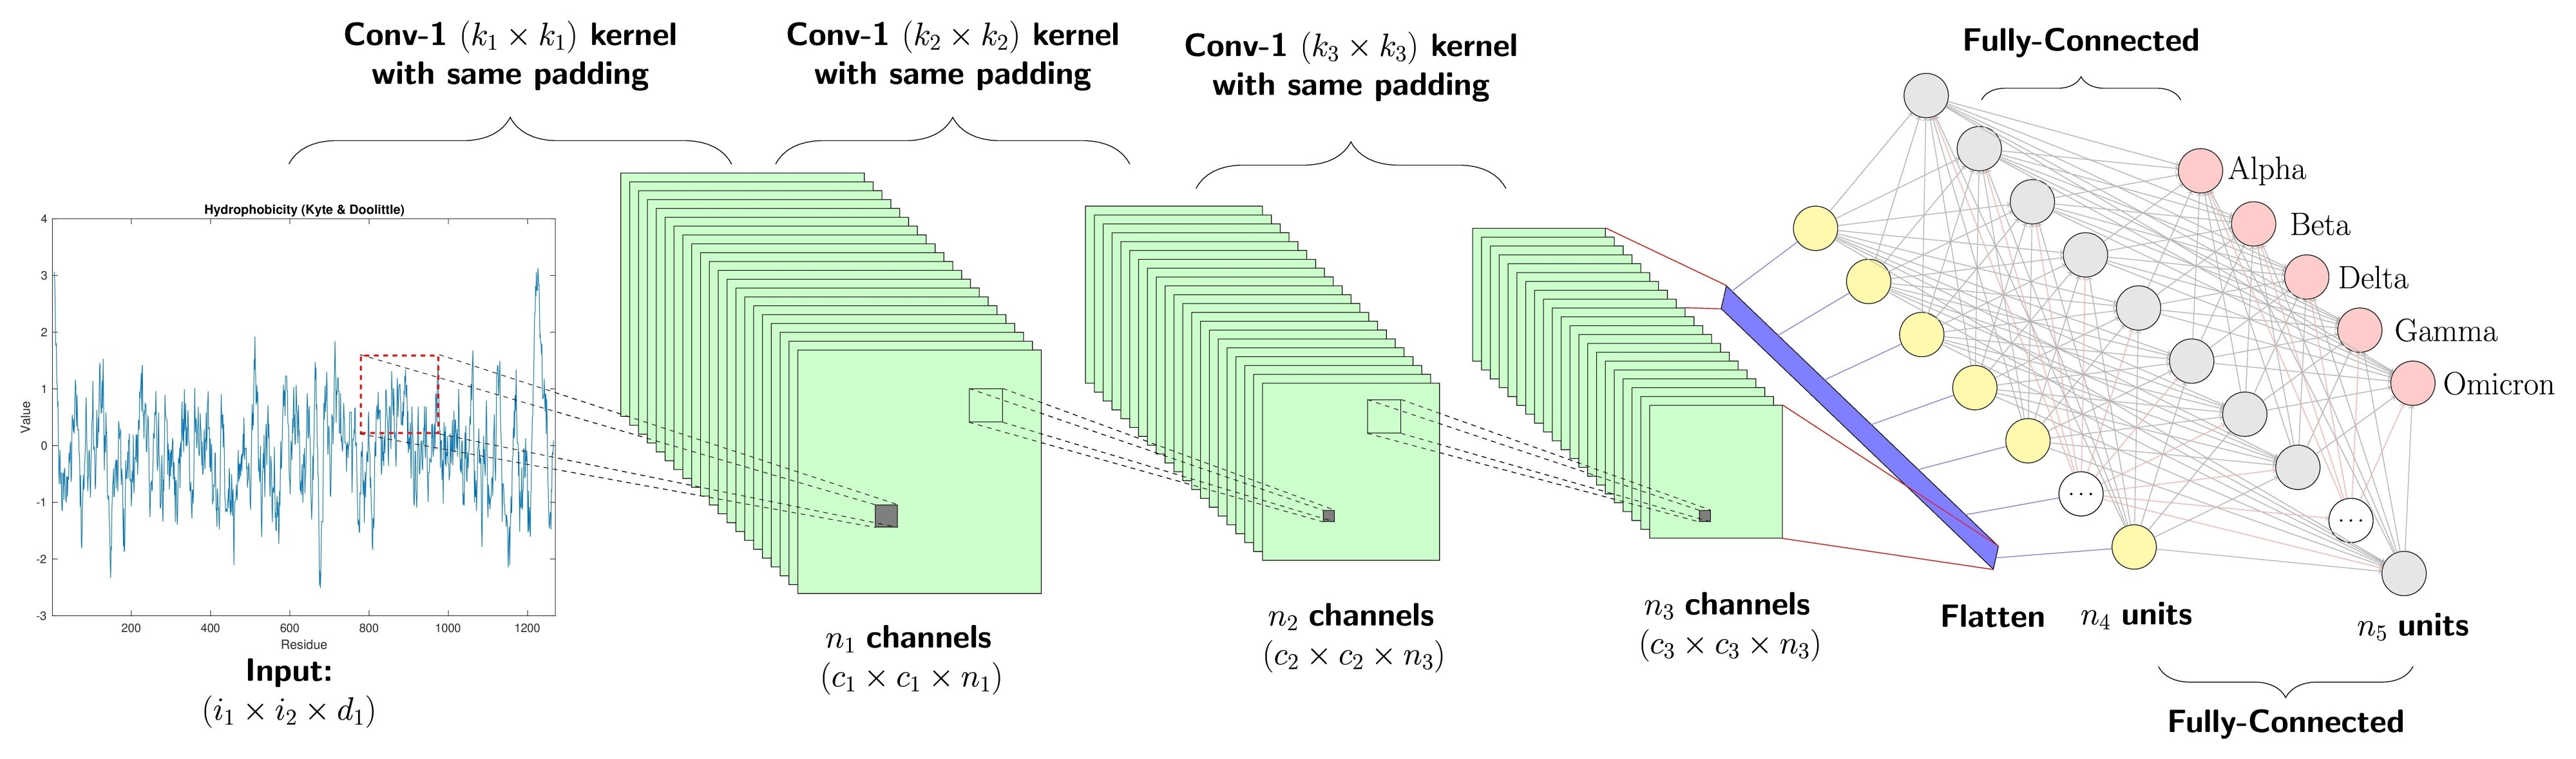
\includegraphics[width=0.8\textwidth]{2_2_convolution.jpeg}
    \caption{Minh họa các phép toán tích chập và gộp trong CNN.}
    \label{fig:cnn_ops}
\end{figure}

\subsubsection{Mô hình dựa trên Transformer}
Vision Transformer (ViT) chia ảnh thành các miếng vá, xử lý như chuỗi token, sử dụng cơ chế Self-Attention: $\text{Attention}(Q, K, V) = \text{softmax}\left(\frac{QK^T}{\sqrt{d_k}}\right)V$, với $Q, K, V$ là ma trận Query, Key, Value.\autocite{dosovitskiy2021} ViT vượt qua giới hạn cục bộ của CNN bằng cách học mối quan hệ toàn cục.

\begin{figure}[h]
    \centering
    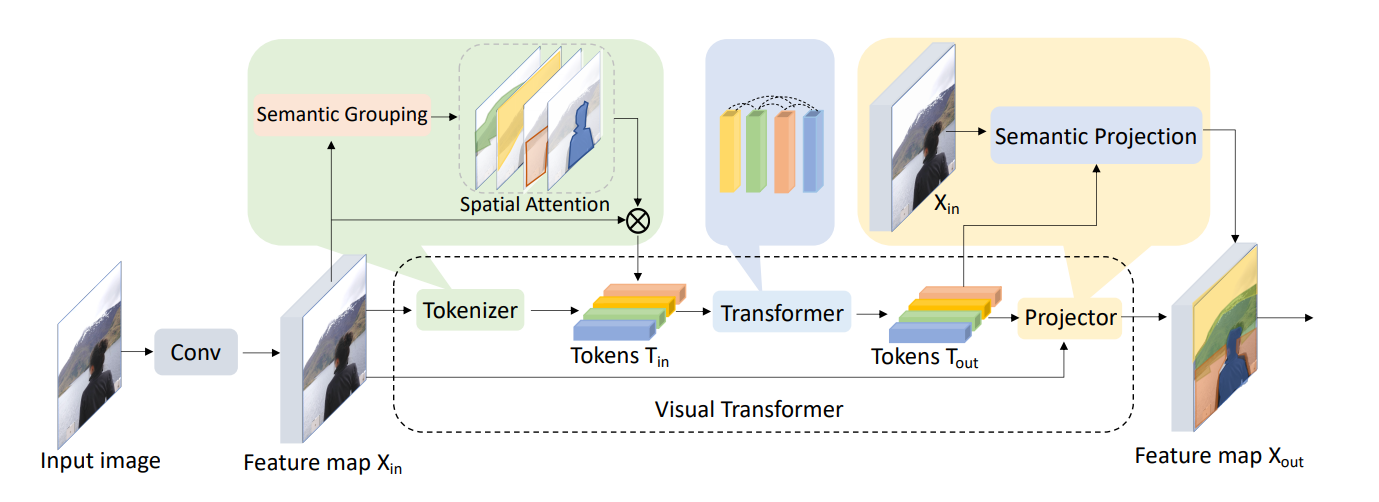
\includegraphics[width=0.9\textwidth]{visual_transformer.png}
    \caption{Kiến trúc Vision Transformer chuyển đổi hình ảnh thành chuỗi token.}
    \label{fig:vit_arch}
\end{figure}

\subsubsection{Mô hình Phân tích Cấp cao}
U-Net dùng encoder-decoder cho phân đoạn pixel-wise.\autocite{ronneberger2015} Optical flow (Horn-Schunck) tính chuyển động: $I_x u + I_y v + I_t = 0$.\autocite{horn1981} Quyết định dựa trên SVM hoặc ngưỡng trên đặc trưng.\autocite{szeliski2010}

\subsection{Các tập dữ liệu phổ biến và thước đo đánh giá mô hình}
\begin{itemize}
    \item \textbf{Tập dữ liệu}:
    \begin{itemize}
        \item ImageNet: Hơn 14 triệu ảnh, 20,000 lớp.\autocite{deng2009}
        \item COCO: Phát hiện và phân đoạn đối tượng.\autocite{lin2014}
        \item MPII, COCO Keypoints: Ước lượng tư thế người.\autocite{lin2014}
    \end{itemize}
    \item \textbf{Metrics}:
    \begin{itemize}
        \item IoU: $\frac{\text{Area of Overlap}}{\text{Area of Union}}$.\autocite{lin2014}
        \item mAP: Trung bình Average Precision trên các lớp.\autocite{lin2014}
        \item F1-score: Trung bình điều hòa Precision và Recall.\autocite{szeliski2010}
        \item OKS: Đo lường độ chính xác khớp trong HPE.\autocite{lin2014}
    \end{itemize}
\end{itemize}

Ví dụ thực tế: Hệ thống tự lái dùng CNN để nhận diện làn đường từ cạnh và gradient, kết hợp optical flow để dự đoán chuyển động.\autocite{redmon2016}

\section{Nhận diện Tư thế Người và Phát hiện Té ngã}
\label{sec:pose_fall_system}

Mục này trình bày tổng quan về nhận diện tư thế người (Human Pose Estimation - HPE), giải pháp thời gian thực MediaPipe Pose, xây dựng thuật toán phát hiện té ngã dựa trên đặc trưng động học (kinematic) và tư thế (postural), cùng mô tả chi tiết hệ thống tích hợp.

\subsection{Nhận diện Tư thế Người (Human Pose Estimation)}

Nhận diện tư thế người là một lĩnh vực then chốt trong thị giác máy tính, nhằm xác định vị trí và hướng các khớp (joints) và bộ phận cơ thể từ hình ảnh hoặc chuỗi video. Khả năng này là nền tảng cho các ứng dụng giám sát an toàn, phân tích chuyển động, và nhận diện hành vi bất thường (như té ngã).

\subsubsection{Khái niệm và Định nghĩa}

Pose Estimation ước lượng vị trí của các bộ phận cơ thể trong không gian 2D hoặc 3D, được biểu diễn qua tập hợp các \textbf{keypoints} (khớp/điểm mốc):
\begin{equation}
\mathcal{K} = \{k_1, k_2, ..., k_n\}, \quad k_i = (x_i, y_i, z_i, c_i)
\end{equation}
trong đó $(x_i, y_i, z_i)$ là tọa độ không gian (với $z_i$ là tọa độ chiều sâu tương đối) và $c_i$ là độ tin cậy (\textbf{confidence score}) của keypoint thứ $i$.

\paragraph{Phân loại Phương pháp HPE:}
\begin{itemize}
    \item \textbf{Top-down Approach:} Đầu tiên phát hiện đối tượng người, sau đó ước lượng keypoints cho từng hộp giới hạn (bounding box) của người. (VD: Mask R-CNN, MediaPipe).
    \item \textbf{Bottom-up Approach:} Đầu tiên phát hiện tất cả các keypoints, sau đó nhóm chúng lại để tạo thành tư thế của từng người. (VD: OpenPose).
\end{itemize}

%%%%%%%%%%%%%%%%%%%%%%%%%%%%%%%%%%%%%%%%%%%%%%%%%%%%%%%%%%%%%%%%%%%%%%%%%%%%%%%%
\subsection{MediaPipe Pose Estimation cho Ứng dụng Thời gian thực}

MediaPipe Pose, dựa trên mô hình **BlazePose** của Google, được tối ưu hóa để cung cấp giải pháp HPE 3D nhanh và chính xác trong môi trường thời gian thực trên nhiều nền tảng (Mobile, Web, Desktop).

\subsubsection{Kiến trúc xử lý Graph-based}

MediaPipe sử dụng kiến trúc xử lý dữ liệu dựa trên đồ thị (Graph-based Processing), nơi các nhiệm vụ được tổ chức thành một chuỗi các module:
\begin{itemize}
    \item \textbf{Nodes (Calculator):} Các module xử lý độc lập thực hiện các nhiệm vụ cụ thể (VD: Phát hiện đối tượng, Ước lượng điểm mốc).
    \item \textbf{Edges (Packet Stream):} Các luồng dữ liệu (packets) được truyền tải giữa các Nodes, đảm bảo đồng bộ hóa và nhất quán dữ liệu giữa các bước.
\end{itemize}

\subsubsection{Các thành phần Mô hình Chính}

\paragraph{Pose Detection Model (Localization):} Nhiệm vụ là phát hiện sự hiện diện và xác định \textbf{Vùng quan tâm (ROI)} chứa người trong khung hình.
\begin{itemize}
    \item Input: Khung hình RGB.
    \item Output: Bounding box và xác suất hiện diện của người.
\end{itemize}

\paragraph{Pose Landmark Model (BlazePose):} Mô hình ước lượng các điểm mốc chính xác trên ROI đã xác định.
\begin{itemize}
    \item Output: 33 keypoints 3D $(x, y, z, visibility)$.
    \item Hàm mất mát (\textbf{Loss Function}) tổng hợp:
    \begin{equation}
    \mathcal{L}_{\text{total}} = \lambda_1 \mathcal{L}_{\text{coord}} + \lambda_2 \mathcal{L}_{\text{confidence}} + \lambda_3 \mathcal{L}_{\text{depth}}
    \end{equation}
\end{itemize}

\paragraph{Pose Tracking Model:} Dự đoán ROI cho khung hình tiếp theo dựa trên pose hiện tại. Việc này giúp giảm đáng kể chi phí tính toán (computational cost) bằng cách tránh chạy mô hình phát hiện đầy đủ ở mỗi khung hình.

\subsubsection{Thuật toán Hậu xử lý (Post-processing)}

\paragraph{Temporal Smoothing (One Euro Filter):} Áp dụng bộ lọc thời gian để làm mịn tín hiệu tọa độ keypoint qua các khung hình, loại bỏ nhiễu và tăng độ ổn định của chuyển động ước tính.

\paragraph{3D Coordinate Estimation:} Chiều sâu tương đối $z$ được chuẩn hóa dựa trên kích thước cơ thể (thường là khoảng cách giữa hông).

%%%%%%%%%%%%%%%%%%%%%%%%%%%%%%%%%%%%%%%%%%%%%%%%%%%%%%%%%%%%%%%%%%%%%%%%%%%%%%%%
\subsection{Thuật toán Phát hiện Té ngã Multi-stage}

Hệ thống phát hiện té ngã sử dụng các đặc trưng động học (Kinematic) và tư thế (Postural) được trích xuất từ dữ liệu keypoints 3D (từ MediaPipe) để đưa ra quyết định qua nhiều giai đoạn. $\Delta t$ được định nghĩa là thời gian trôi qua giữa hai khung hình liên tiếp ($1/FPS$).

\subsubsection{Trích xuất Đặc trưng Sinh học (Feature Engineering)}

\paragraph{Kinematic Features (Đặc trưng Động học):} Phản ánh tốc độ và gia tốc trong quá trình té ngã.
\begin{itemize}
    \item \textbf{Vận tốc COM ($\vec{v}_{\text{COM}}$) và Gia tốc COM ($a_{\text{total}}$):}
    \begin{align}
    \vec{v}_{\text{COM}}(t) &= \frac{\vec{p}_{\text{COM}}(t) - \vec{p}_{\text{COM}}(t-\Delta t)}{\Delta t} \\
    \vec{p}_{\text{COM}} &= \frac{\sum_i w_i \vec{p}_i c_i}{\sum_i w_i c_i} \quad (\text{Với } w_i \text{ là trọng số khối lượng sinh học}) \\
    a_{\text{total}}(t) &= \frac{\|\vec{v}_{\text{COM}}(t) - \vec{v}_{\text{COM}}(t-\Delta t)\|}{\Delta t}
    \end{align}
\end{itemize}

\paragraph{Postural Features (Đặc trưng Tư thế):} Phản ánh hình dạng cơ thể và độ cao sau khi té ngã.
\begin{itemize}
    \item \textbf{Tỷ lệ Khía cạnh (Aspect Ratio - AR):} Tỷ lệ giữa chiều rộng và chiều cao của hộp giới hạn người, tăng vọt khi người nằm ngang.
    \item \textbf{Góc Nghiêng Cơ thể ($\theta_{\text{body}}$):} Góc tạo bởi trục cơ thể (vai-hông) so với phương thẳng đứng.
    \item \textbf{Độ giảm chiều cao ($\Delta h_{\text{head}}$):} Sự thay đổi vị trí của đầu so với trạng thái ban đầu.
\end{itemize}

\subsubsection{Thuật toán Phát hiện Té ngã Ba Giai đoạn}

\paragraph{Stage 1: Pre-fall Detection (Phát hiện Sớm)}
Kiểm tra các dấu hiệu ban đầu của sự mất kiểm soát, chủ yếu dựa vào tốc độ và gia tốc của Trung tâm Khối lượng (COM).

\paragraph{Stage 2: Fall Event Verification (Xác nhận Sự kiện Té ngã)}
Nếu Stage 1 là True, kiểm tra các đặc trưng tư thế (AR, $\theta_{\text{body}}$) để xác nhận trạng thái cơ thể chuyển từ đứng/đi sang nằm ngang.

\paragraph{Stage 3: Post-fall Inactivity Check (Kiểm tra Bất động sau té ngã)}
Sau khi té ngã được xác nhận (Stage 2 là True), hệ thống theo dõi mức độ chuyển động trong một khoảng thời gian ($T_{\text{window}}$). Nếu sự chuyển động thấp hơn ngưỡng $M_{th}$ trong thời gian dài, cảnh báo được kích hoạt, loại trừ các trường hợp ngồi hoặc nằm chủ động.

\subsection{Triển khai và Tối ưu hóa Hệ thống Tích hợp}

\subsubsection{Chuỗi Xử lý Dữ liệu (Data Flow Pipeline)}
Hệ thống được thiết kế theo kiến trúc module để dễ dàng tích hợp và tối ưu hóa hiệu suất:
\begin{equation}
\text{Video Stream} \xrightarrow{\text{MediaPipe}} \text{Keypoints} 
\xrightarrow[\text{Kinematic/Postural}]{3\text{D/Temporal Filtering}} \text{Feature Extraction} 
\xrightarrow{\text{Multi-stage Logic}} \text{Decision Engine} 
\xrightarrow{\text{Alert System}} \text{Response}
\end{equation}

\subsubsection{Tối ưu hóa Tham số (Parameter Tuning)}
Việc điều chỉnh các ngưỡng ($V_{th}, A_{th}, AR_{th}, \dots$) là rất quan trọng. Việc sử dụng \textbf{Ngưỡng Thích ứng (Adaptive Thresholds)} $V_{th}^{adaptive}(t)$ (phụ thuộc vào độ tin cậy của keypoints $c_i$) có thể cải thiện độ chính xác trong các môi trường nhiễu hoặc ánh sáng yếu.

\section{Cơ sở Lý thuyết về Phần cứng và Kiến trúc Hệ thống Phát hiện Té ngã}
\label{sec:hardware_theory}

Mục này cung cấp kiến thức nền tảng về phần cứng, các loại cảm biến và module truyền thông được sử dụng trong hệ thống phát hiện té ngã.

\subsection{Tổng quan Kiến trúc Hệ thống Phát hiện Té ngã}
Hệ thống phát hiện té ngã hiện đại thường được phân loại thành hai nhóm chính: \textbf{Hệ thống dựa trên Camera} và \textbf{Hệ thống dựa trên Thiết bị đeo}. Báo cáo này tích hợp cả hai, bao gồm các thành phần cốt lõi:
\begin{enumerate}
    \item \textbf{Thiết bị Thu thập Dữ liệu}: Thu thập dữ liệu chuyển động (IMU) và/hoặc hình ảnh (Camera).
    \item \textbf{Máy chủ Xử lý}: Thực hiện các thuật toán học sâu và logic ra quyết định phức tạp.
    \item \textbf{Hệ thống Truyền thông}: Đảm bảo luồng dữ liệu hai chiều và kích hoạt cảnh báo.
\end{enumerate}

\subsection{Cảm biến và Xử lý Dữ liệu Sơ cấp tại biên}

\subsubsection{Vi điều khiển và Xử lý Cục bộ}
\textbf{ESP32 (hoặc ESP32-S3)} được chọn làm bộ điều khiển trung tâm nhờ kiến trúc \textbf{lõi kép Xtensa LX6} (hoặc S3), cho phép xử lý song song. Một lõi được dành riêng cho các tác vụ thời gian thực như đọc và tiền xử lý dữ liệu cảm biến (ví dụ: \textbf{Kalman Filter} để ước tính hướng và trạng thái), trong khi lõi còn lại quản lý các giao tiếp không dây (Wi-Fi, Bluetooth) và giao thức \textbf{MQTT} hoặc \textbf{HTTP}, giảm thiểu độ trễ.

\subsubsection{Cảm biến Đo lường Quán tính (IMU)}
\textbf{IMU (Inertial Measurement Unit)} là thành phần chính trong hệ thống đeo người, cung cấp dữ liệu về động học của cơ thể. IMU tích hợp:
\begin{itemize}
    \item \textbf{Gia tốc kế}: Đo gia tốc tuyến tính. Gia tốc thô được hiệu chuẩn để chuyển từ giá trị số nguyên sang đơn vị thực tế ($g$).
    \item \textbf{Con quay hồi chuyển}: Đo tốc độ góc, dựa trên \textbf{hiệu ứng Coriolis}.
    \item \textbf{Từ kế}: Cung cấp tham chiếu hướng từ trường để hiệu chỉnh sai số trôi của con quay hồi chuyển (thường thông qua thuật toán \textbf{Sensor Fusion} như Bộ lọc Madgwick hoặc Kalman).
\end{itemize}

Dữ liệu thô sau khi xử lý (ví dụ: trung bình hóa) được biểu diễn dưới dạng vector 3D:
\[
\mathbf{a} = [a_x, a_y, a_z], \quad
\boldsymbol{\omega} = [\omega_x, \omega_y, \omega_z]
\]

\paragraph{Phát hiện Té ngã dựa trên Ngưỡng IMU}
Tại tầng vi điều khiển, té ngã được phát hiện sơ bộ bằng cách phân tích sự thay đổi đột ngột của \textbf{Gia tốc Tổng (Magnitude of Acceleration)} và tốc độ góc:
\begin{itemize}
    \item \textbf{Shock Event}: Gia tốc tổng vượt ngưỡng cao ($a_{\text{shock}}$): $\|\mathbf{a}\| > a_{\text{shock}}$.
    \item \textbf{Post-fall State}: Gia tốc tổng sau đó giảm về gần 1g (biểu thị trạng thái nằm ngang) trong khi tốc độ góc có thay đổi lớn.
\end{itemize}
\[
\|\mathbf{a}\| = \sqrt{a_x^2 + a_y^2 + a_z^2}
\]

\subsubsection{Cảm biến Định vị Vị trí (GPS)}
Module GPS (ví dụ: u-blox NEO-6M) sử dụng nguyên lý \textbf{Đo tam giác} để xác định vị trí địa lý của thiết bị dựa trên tín hiệu từ ít nhất bốn vệ tinh. Dữ liệu đầu ra là chuỗi \textbf{NMEA}, cung cấp tọa độ Kinh độ/Vĩ độ và độ cao, là thông tin quan trọng cho dịch vụ cứu hộ khẩn cấp.

\subsection{Hệ thống Camera và Xử lý Máy chủ}

\subsubsection{Hệ thống Camera}
Camera nhúng (\textbf{ESP32-S3 + OV5640 5MP}) cung cấp dữ liệu hình ảnh được nén theo chuẩn \textbf{JPEG}. Dữ liệu này là luồng byte được truyền tải qua Wi-Fi bằng các giao thức như \textbf{RTSP} hoặc \textbf{HTTP/MJPEG stream}, phục vụ cho việc \textbf{Xác minh Hình ảnh} trên máy chủ.

\subsubsection{Kiến trúc Máy chủ Xử lý}
Máy chủ là nơi thực hiện các thuật toán phức tạp như Ước lượng tư thế người (HPE) và Học sâu, đảm bảo độ chính xác cao.
\begin{itemize}
    \item \textbf{Phần cứng}: Sử dụng máy chủ đám mây (AWS, Google Cloud) hoặc máy tính nhúng mạnh mẽ (NVIDIA Jetson Nano) có \textbf{GPU} để tăng tốc tính toán Tensor.
    \item \textbf{Phần mềm Học sâu}: Nền tảng \textbf{TensorFlow/PyTorch} kết hợp với thư viện \textbf{OpenCV}.
    \item \textbf{Xử lý Dữ liệu Lớn}: Máy chủ tiếp nhận luồng dữ liệu \textbf{JSON/MQTT} (từ IMU) và luồng \textbf{JPEG} (từ Camera). Việc tổng hợp và đồng bộ hóa hai luồng dữ liệu này là chìa khóa để xác minh té ngã và giảm thiểu báo động giả (False Positives).
\end{itemize}

\subsection{Hệ thống Truyền thông và Cơ chế Dự phòng}

\subsubsection{Module Truyền thông Đa dạng}
\begin{itemize}
    \item \textbf{Wi-Fi (ESP32)}: Kênh chính để truyền tải dữ liệu dung lượng lớn (video/hình ảnh) và giao tiếp \textbf{MQTT} với máy chủ.
    \item \textbf{Module Di động (4G/LTE - EC800K)}: Đóng vai trò là \textbf{Kênh Dự phòng}. Nó hỗ trợ định vị GPS và quan trọng nhất là kích hoạt \textbf{cuộc gọi khẩn cấp tự động} hoặc gửi \textbf{SMS cảnh báo} bằng \textbf{AT commands}, đảm bảo cảnh báo được gửi đi ngay cả khi mạng Wi-Fi không khả dụng.
\end{itemize}

\subsubsection{Liên kết Tổng thể và Logic Dự phòng}
Hệ thống vận hành theo nguyên lý tích hợp và dự phòng:
\begin{enumerate}
    \item \textbf{Thu thập/Xử lý Sơ cấp}: ESP32 thu thập IMU/Camera và thực hiện phát hiện té ngã dựa trên ngưỡng IMU.
    \item \textbf{Quyết định Truyền thông}: Nếu té ngã được phát hiện, dữ liệu được truyền đến máy chủ qua kênh Wi-Fi (Ưu tiên) hoặc 4G (Dự phòng).
    \item \textbf{Xác minh Máy chủ}: Máy chủ tiến hành phân tích hình ảnh (HPE) kết hợp với dữ liệu IMU để xác minh té ngã (Multi-stage Fall Detection Logic).
    \item \textbf{Kích hoạt Cảnh báo}: Nếu xác nhận té ngã, máy chủ ra lệnh cho ESP32 kích hoạt Module EC800K gửi cảnh báo (SMS/Cuộc gọi), hoàn tất chu trình cứu hộ.
\end{enumerate}

\subsubsection{Môi trường Phát triển Phần mềm Nhúng}
Việc phát triển phần mềm cho các vi điều khiển như ESP32 đòi hỏi một framework chuyên biệt. \textbf{ESP-IDF (Espressif IoT Development Framework)} được chọn làm môi trường phát triển chính thay vì các IDE đơn giản hơn (như Arduino IDE) vì những lý do sau:
\begin{itemize}
    \item \textbf{Hỗ trợ RTOS}: ESP-IDF tích hợp \textbf{FreeRTOS}, cho phép tận dụng tối đa kiến trúc lõi kép của ESP32 để thực hiện đa nhiệm (ví dụ: một tác vụ xử lý dữ liệu IMU thời gian thực, một tác vụ quản lý kết nối Wi-Fi).
    \item \textbf{Truy cập Cấp thấp (Low-level Access)}: Cho phép truy cập trực tiếp và tối ưu hóa các thanh ghi phần cứng (Registers), cần thiết cho việc cấu hình cảm biến IMU (I2C/SPI) và tinh chỉnh các giao thức mạng phức tạp (MQTT/HTTP) ở mức độ chi tiết cao, đảm bảo hiệu suất thời gian thực.
\end{itemize}
Việc lựa chọn môi trường này là nền tảng để xây dựng các mô-đun phần mềm chuyên biệt, sẽ được trình bày chi tiết trong Chương 3.

\subsection{Tóm tắt Chương và Cơ sở cho Triển khai đề tài}
\label{sec:chapter_conclusion}

Chương này đã thiết lập nền tảng lý thuyết toàn diện, tạo cơ sở khoa học cho việc thiết kế và triển khai hệ thống phát hiện té ngã tích hợp. Những kiến thức cốt lõi đã được trình bày bao gồm:
\begin{itemize}
    \item \textbf{Cơ sở Thị giác Máy tính:} Nắm vững kiến trúc CNN và Transformer, là nền tảng cho việc xử lý hình ảnh và nhận diện tư thế người.
    \item \textbf{Phương pháp Ước lượng Tư thế Người (HPE):} Chi tiết về MediaPipe Pose (BlazePose) như một giải pháp thời gian thực, cung cấp tọa độ 3D $\mathcal{K}$ (keypoints) làm dữ liệu đầu vào cho các thuật toán phân tích hành vi.
    \item \textbf{Phần cứng Hệ thống Nhúng:} Phân tích vai trò của ESP32/ESP32-S3, cảm biến IMU (Gia tốc, Con quay, Từ kế) và Module Truyền thông (Wi-Fi, 4G), cùng với các nguyên lý xử lý tín hiệu sơ cấp như tính toán Gia tốc Tổng.
\end{itemize}

Tất cả các thành phần lý thuyết này sẽ được tích hợp trong Chương tiếp theo. Cụ thể, mô hình lý thuyết về các \textbf{đặc trưng động học} và \textbf{tư thế} (Kinematic \& Postural Features) sẽ được chuyển hóa thành các mô-đun phần mềm trên nền tảng ESP-IDF và các Framework. Chương tiếp theo, \textbf{Thiết kế và Phương pháp luận Triển khai}, sẽ tập trung vào việc kiến trúc hóa hệ thống, chi tiết hóa cấu trúc mã nguồn, và mô tả quy trình thực nghiệm được tiến hành để biến các nguyên lý cơ sở thành một giải pháp phát hiện té ngã thời gian thực, đáng tin cậy.


\chapter{Thuc hien he thong canh bao te nga}

\section{1 System Architecture}


\section{Thực hiện phần cứng}
\label{sec:hardware_implementation}

Hệ thống Phát hiện té ngã và Cảnh báo (FDAS) được triển khai theo kiến trúc mô-đun với hai module chính hoạt động độc lập, đảm bảo linh hoạt, khả năng giám sát rộng và duy trì hoạt động khi một module gặp sự cố. Module I tập trung vào thu thập dữ liệu chuyển động và định vị, trong khi Module II xử lý hình ảnh để xác nhận sự kiện té ngã.

\subsection{Module I: Thiết bị đeo / Cảm biến}
\label{ssec:module_one}

Module I là thiết bị phát hiện ban đầu, thiết kế nhỏ gọn để người dùng mang theo. Các thành phần chính bao gồm:

\begin{figure}[H]
    \centering
    \includegraphics[width=0.7\textwidth]{figures/module1_block_diagram-crop.pdf}
    \caption{Sơ đồ khối Module I: Thiết bị đeo / Cảm biến}
    \label{fig:module1_block_diagram}
\end{figure}

\begin{itemize}
    \item \textbf{ESP32-DevKitC-1}: Bộ vi điều khiển trung tâm, tích hợp Wi-Fi và Bluetooth, chi phí thấp, hiệu suất ổn định.
    \item \textbf{MPU6050}: Cảm biến IMU 6 trục, đo gia tốc và tốc độ góc, tích hợp bộ xử lý chuyển động DMP.
    \item \textbf{Module GPS/4G (EC800K)}: Thu thập tọa độ GPS và gửi dữ liệu cảnh báo qua mạng 4G.
    \item \textbf{Các thành phần hỗ trợ}: Buzzer và LED onboard để phản hồi tức thì khi phát hiện sự kiện.
\end{itemize}

\begin{figure}[H]
    \centering
    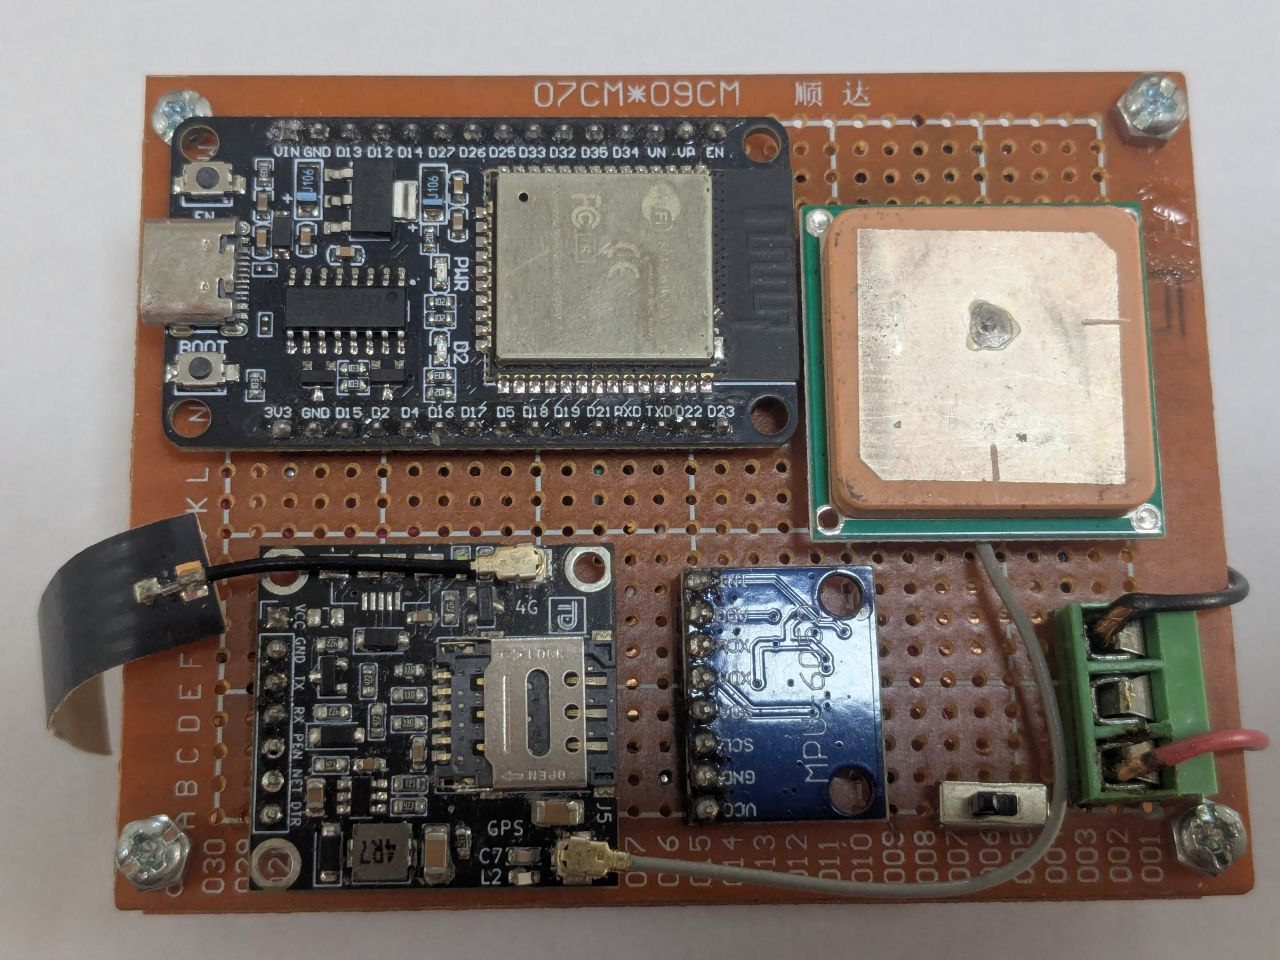
\includegraphics[width=0.8\textwidth]{figures/real_board1.jpg}
    \caption{Hình ảnh thực tế Module I đã hoàn thiện}
    \label{fig:module1_photo}
\end{figure}

Sơ đồ nguyên lý chi tiết (schematic) được vẽ bằng KiCad, đính kèm trong \textbf{Phụ lục B}.

\subsection{Module II: Camera giám sát}
\label{ssec:module_two}

Module II xác nhận sự kiện té ngã bằng hình ảnh, đặt ở khu vực giám sát trọng yếu. Các thành phần chính:

\begin{itemize}
    \item \textbf{ESP32-S3-N16R8}: Vi điều khiển mạnh mẽ, tích hợp Wi-Fi/Bluetooth, hỗ trợ PSRAM và giao diện camera chuyên dụng, tối ưu xử lý luồng dữ liệu hình ảnh.
    \item \textbf{Camera OV5640}: Cảm biến 5MP, hỗ trợ nhiều kích thước khung hình (QQVGA đến UXGA), giao tiếp dữ liệu song song 8-bit với SCCB, xung nhịp 20 MHz.
\end{itemize}

\paragraph{Sơ đồ kết nối phần cứng}
Bảng \ref{tab:pin_mapping} tóm tắt sơ đồ chân giữa ESP32-S3 và OV5640.

\begin{table}[H]
    \centering
    \caption{Sơ đồ kết nối chân giữa ESP32-S3 và OV5640}
    \label{tab:pin_mapping}
    \begin{tabular}{|l|c|l|}
    \hline
    \textbf{Chức năng} & \textbf{Chân ESP32-S3} & \textbf{Mô tả} \\
    \hline
    XCLK & 15 & Tín hiệu xung nhịp cho camera \\
    SIOD (SDA) & 4 & Dòng dữ liệu I2C \\
    SIOC (SCL) & 5 & Xung nhịp I2C \\
    D0-D7 & 11,9,8,10,12,18,17,16 & Bus dữ liệu 8-bit \\
    VSYNC & 6 & Đồng bộ khung hình dọc \\
    HREF & 7 & Tham chiếu hàng ngang \\
    PCLK & 13 & Xung nhịp điểm ảnh \\
    \hline
    \end{tabular}
\end{table}

\begin{figure}[H]
    \centering
    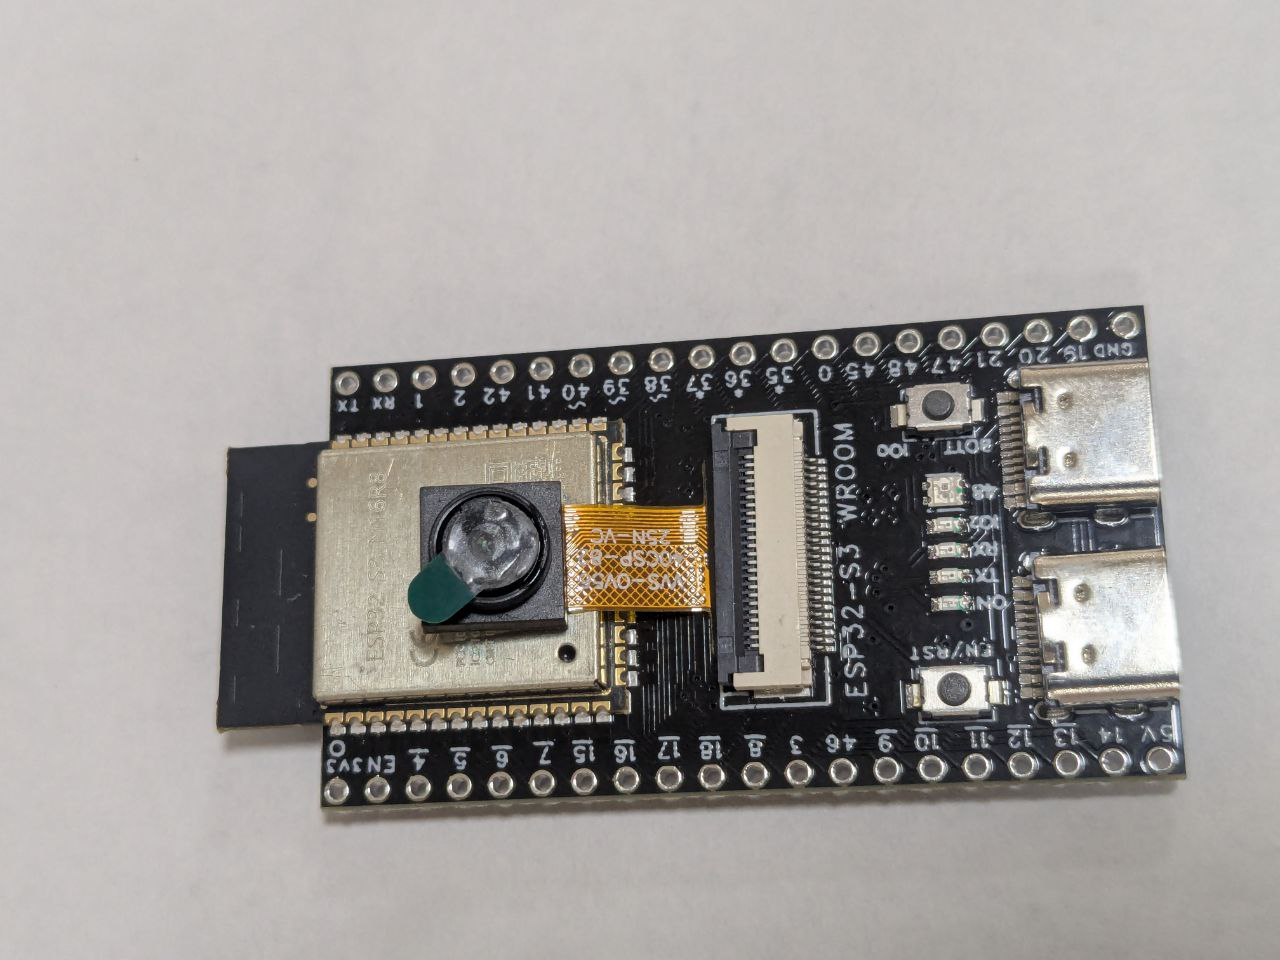
\includegraphics[width=0.8\textwidth]{figures/real_board2.jpg}
    \caption{Hình ảnh thực tế Module II}
    \label{fig:module2_photo}
\end{figure}

\subsection{Bảng tổng hợp các thành phần phần cứng}
\label{ssec:component_summary}

Bảng \ref{tab:hardware_components} tóm tắt các thành phần chính của hai module cùng vai trò và giá thành ước tính.

\begin{table}[H]
    \centering
    \caption{Tổng hợp các thành phần phần cứng}
    \label{tab:hardware_components}
    \begin{tabular}{|l|p{5cm}|p{2cm}|l|}
    \hline
    \textbf{Thành phần} & \textbf{Chức năng} & \textbf{Hình ảnh} & \textbf{Giá thành ước tính (VNĐ)} \\
    \hline
    ESP32-DevKitC-1 & Vi điều khiển chính & 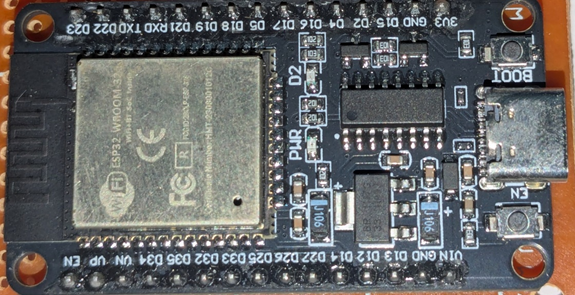
\includegraphics[width=2cm]{figures/real_esp32_c1.png} & 110.000 - 125.000 \\
    MPU6050 & Cảm biến IMU 6 trục & 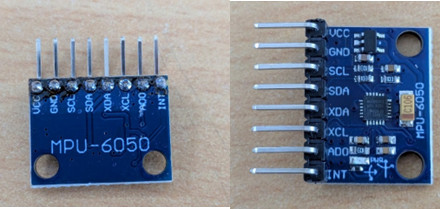
\includegraphics[width=2cm]{figures/real_mpu6050.png} & 45.000 - 55.000 \\
    GPS-antenna & Anten nhận GPS & 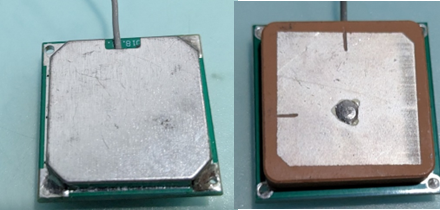
\includegraphics[width=2cm]{figures/real_gps_antenna.png} & 35.000 - 60.000 \\
    Module GPS/4G (EC800K) & Định vị và gửi cảnh báo & 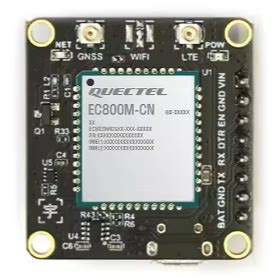
\includegraphics[width=2cm]{figures/real_ec800k.jpg} & ~240.000 \\
    Buzzer & Cảnh báo âm thanh & 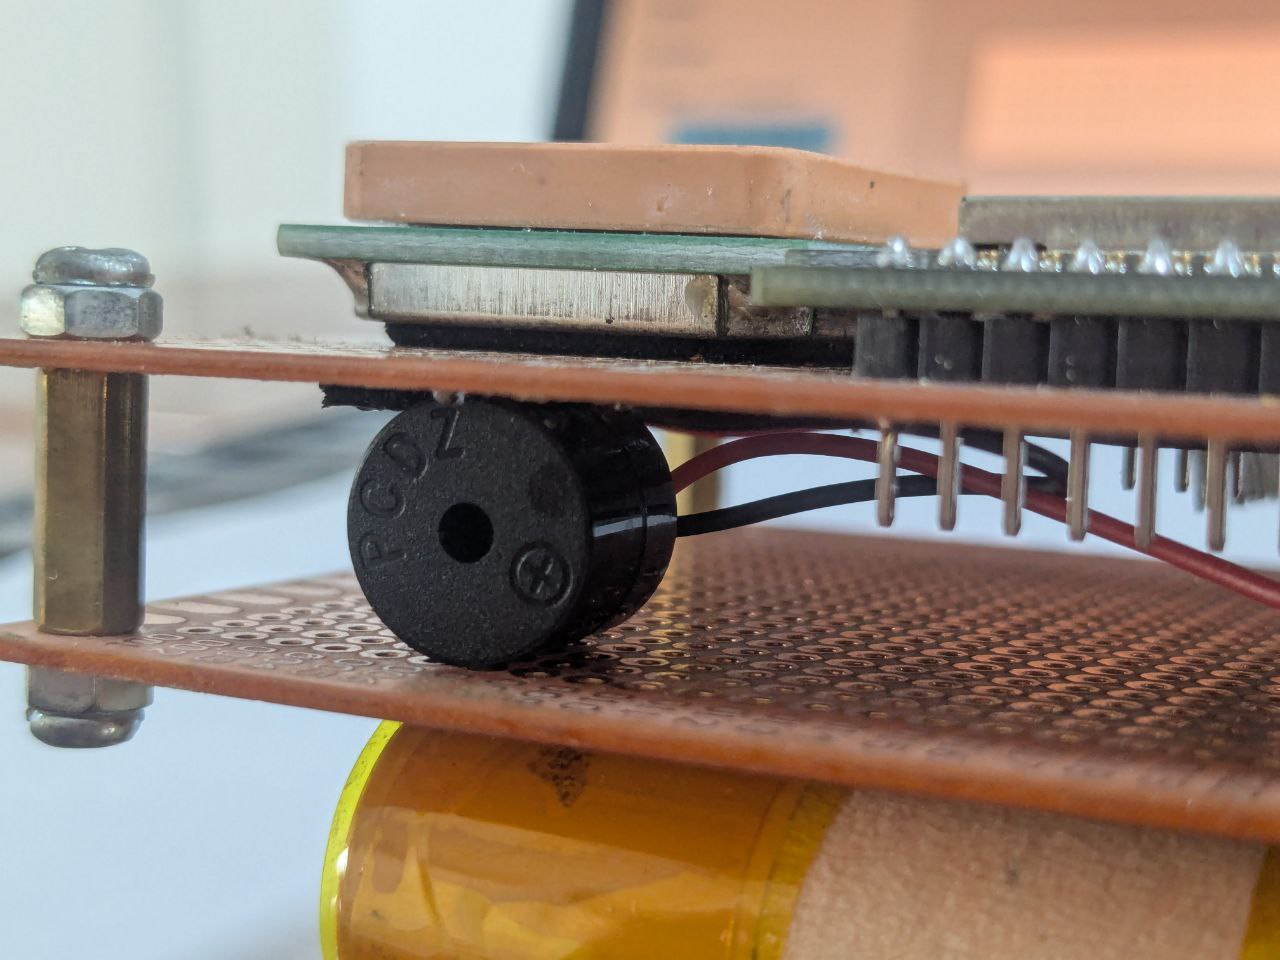
\includegraphics[width=2cm]{figures/real_buzzer.jpg} & 5.000 - 10.000 \\
    ESP32-S3-N16R8 & Vi điều khiển xử lý hình ảnh & 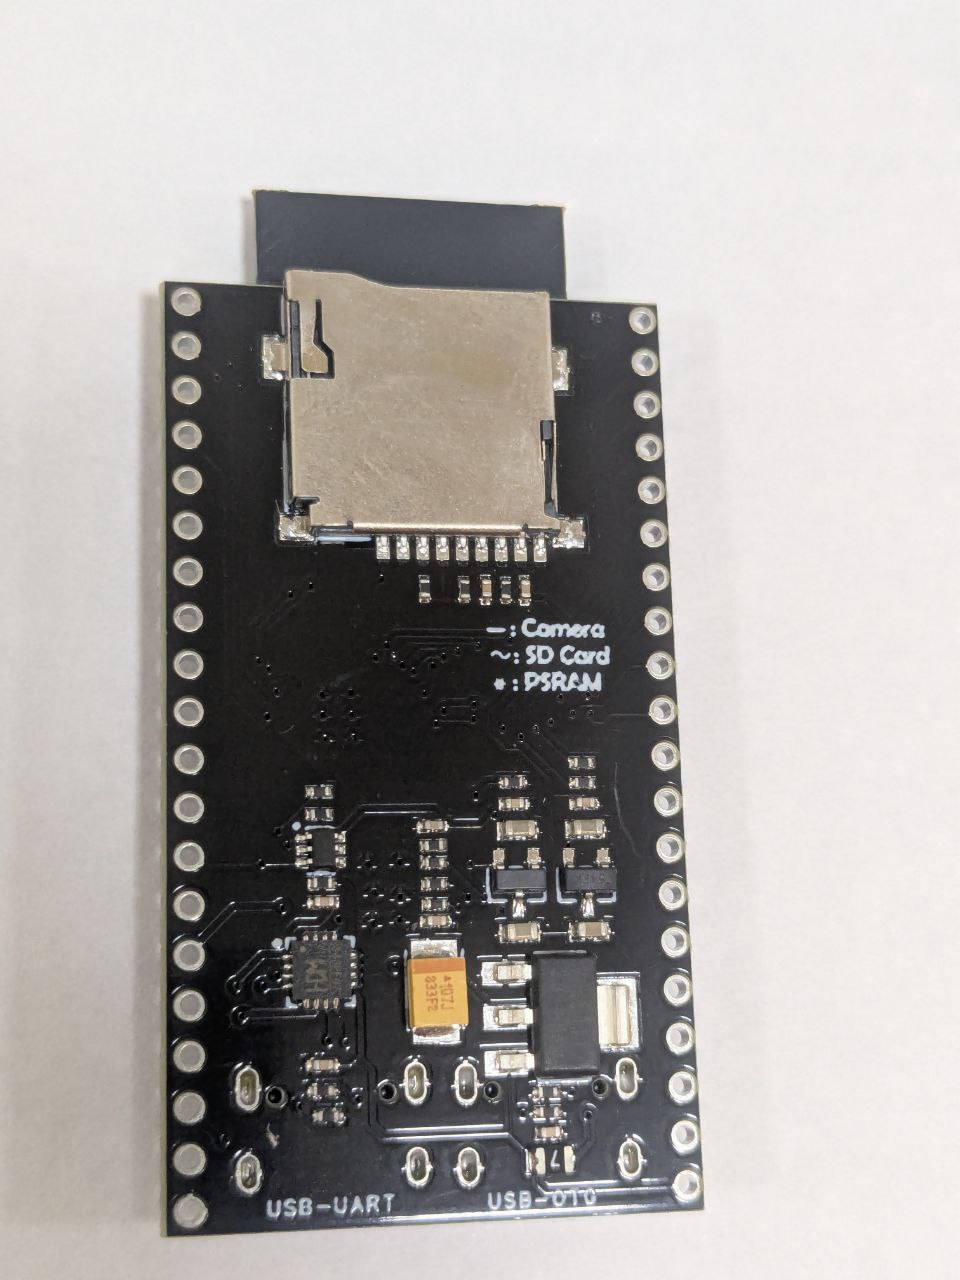
\includegraphics[width=2cm]{figures/real_esp32_s3_2.jpg} & 275.000 - 300.000 \\
    Camera OV5640 & Cảm biến hình ảnh 5MP & 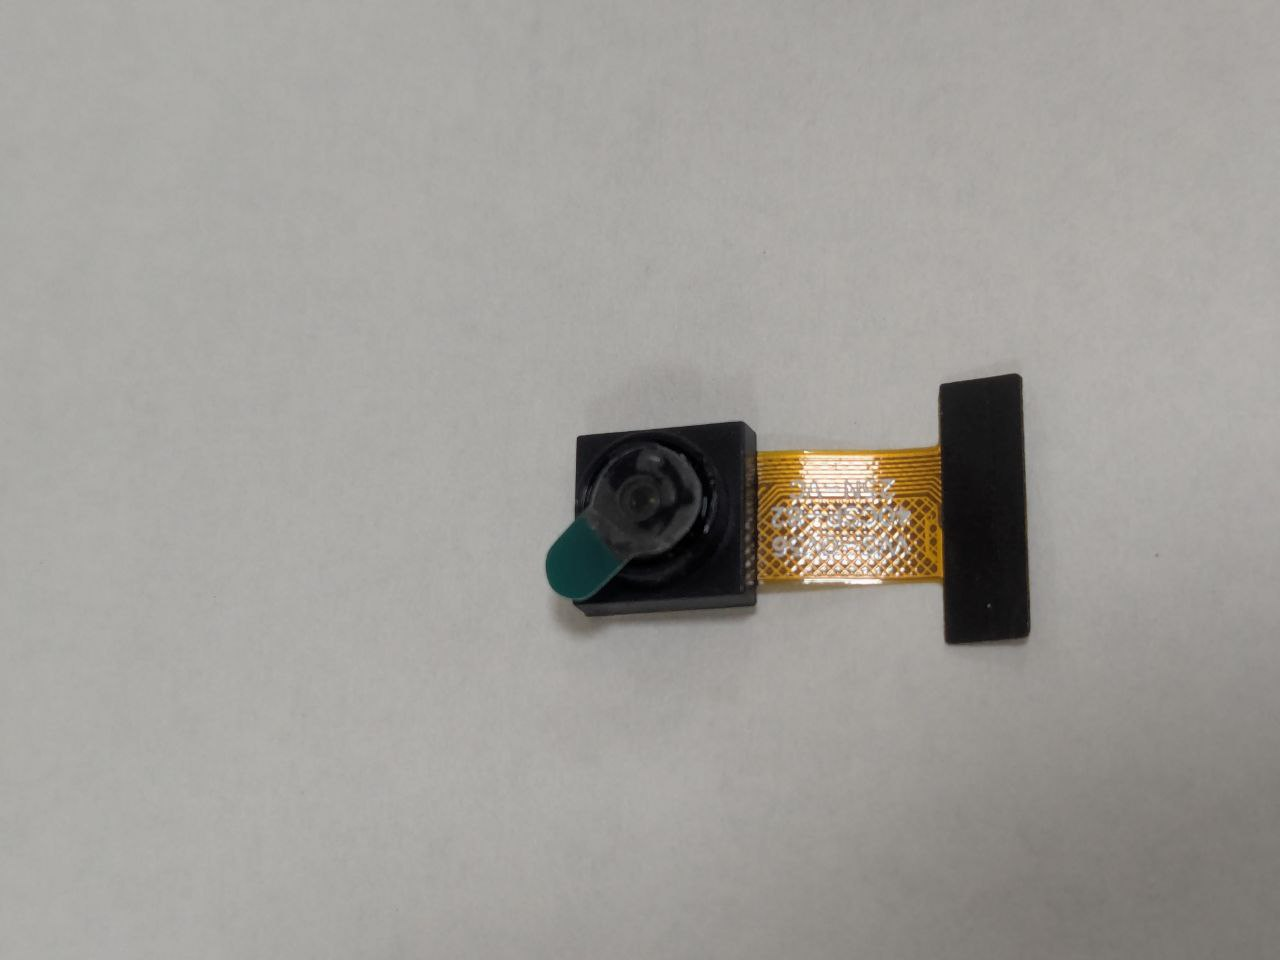
\includegraphics[width=2cm]{figures/real_ov5640.jpg} & 150.000 - 200.000 \\
    \hline
    \end{tabular}
\end{table}

\section{3 Detection Logic}
This is the content for section 3_3_detection_logic.

\section{4 Alerting System}
This is the content for section 3_4_alerting_system.


\chapter[KẾT QUẢ VÀ THỰC NGHIỆM]{THỰC NGHIỆM VÀ ĐÁNH GIÁ KẾT QUẢ HIỆU NĂNG HỆ THỐNG}
\label{chap:results} % Consistent English label

\section*{} % Chapter introduction (un-numbered section)
% This section transitions from the methodology to the results.
Chương trước đã hoàn tất việc thiết kế chi tiết các mô-đun phần cứng, phần mềm. Chương 4 này sẽ tập trung vào việc \textbf{đánh giá hiệu năng thực tế} của hệ thống. Các thử nghiệm được thiết kế nhằm kiểm tra tính khả thi và độ tin cậy của phương pháp tiếp cận đa phương thức được đề xuất. Nội dung chương sẽ trình bày chi tiết về thiết lập thực nghiệm, các tiêu chí đánh giá và phân tích các kết quả thu được

% --- START OF CHAPTER SECTIONS (Input files) ---

\section{Thiết lập thực nghiệm}
\label{sec:experimental_setup}
Trong mục này, chúng tôi trình bày các thành phần \textbf{phần cứng}, \textbf{phần mềm} và \textbf{môi trường thử nghiệm} được sử dụng để triển khai hệ thống phát hiện té ngã.  
Mục tiêu là cung cấp một cái nhìn tổng thể về cách thức xây dựng hệ thống, nhằm đảm bảo quá trình đánh giá hiệu năng ở các mục tiếp theo có cơ sở rõ ràng và có thể tái lập.  

Dữ liệu được thu thập từ cảm biến tại thiết bị đầu cuối, xử lý sơ bộ trên vi điều khiển ESP32 và truyền về máy chủ xử lý trung tâm thông qua giao thức MQTT hoặc kênh SMS khẩn cấp.  
Sơ đồ tổng quan của hệ thống thử nghiệm được minh họa trong Hình~\ref{fig:system_structure}.

\begin{figure}[H]
    \centering
    \includegraphics[width=0.95\textwidth]{figures/resuilt_structure_diagram.pdf}
    \caption{Kiến trúc tổng quan của hệ thống thử nghiệm phát hiện té ngã.}
    \label{fig:system_structure}
\end{figure}

\subsection{Môi trường thử nghiệm}
Các thử nghiệm được thực hiện trong môi trường trong nhà, với nhiều kịch bản té ngã và hoạt động sinh hoạt bình thường. Dữ liệu được ghi nhận để đánh giá:
\begin{itemize}
    \item \textbf{Độ chính xác}: Xác suất hệ thống phát hiện đúng té ngã.
    \item \textbf{Độ trễ}: Thời gian từ khi xảy ra sự kiện đến khi người dùng nhận cảnh báo.
    \item \textbf{Độ ổn định}: Khả năng vận hành liên tục và độ tin cậy trong quá trình thử nghiệm.
\end{itemize}

 % 4.1 New: Experimental setup and metrics

\section{Kết quả kiểm thử từng thành phần}
\label{sec:component_testing}

Trước khi tiến hành phân tích hiệu năng, các thử nghiệm chức năng được thực hiện để xác nhận rằng từng thành phần của hệ thống hoạt động đúng như thiết kế.  
Các log tiêu biểu và hình ảnh minh họa dưới đây cho thấy quá trình khởi tạo, kết nối, truyền dữ liệu định kỳ, phát hiện té ngã, xử lý cảnh báo và truyền hình ảnh.

\subsection{Module cảm biến đeo}
Module Quectel EC800K thuộc phần cứng cảm biến đeo được kiểm tra để xác nhận khả năng giao tiếp AT command, thiết lập kết nối 4G và thu nhận dữ liệu GPS.  

Quy trình kiểm thử bao gồm: khởi tạo UART, kiểm tra thông tin modem và SIM, đánh giá chất lượng sóng, cấu hình APN, kích hoạt PDP context, bật GPS và truy vấn tọa độ, sau đó tắt GPS và ngắt kết nối dữ liệu để tiết kiệm năng lượng.  

Kết quả cho thấy module hoạt động ổn định: thiết bị nhận diện đúng (EC800K), SIM sẵn sàng, tín hiệu mạnh (\texttt{+CSQ: 31,99}), kết nối dữ liệu thành công và thu được tọa độ GPS hợp lệ.

\textbf{Log tiêu biểu:}
\begin{minted}[fontsize=\footnotesize,breaklines]{text}
I (2329) SIM_4G: Received: Quectel EG800K
OK
I (5329) SIM_4G: Received: +CSQ: 31,99
OK
I (28339) SIM_4G: Received: +QIACT: 1,1,1,"9.204.251.200"
OK
I (34349) SIM_4G: Received: +QGPSLOC: 10.88862,106.77975
OK
\end{minted}

\textit{Kết luận:} Module 4G/GPS đã hoạt động đúng chức năng, đảm bảo hệ thống có thể gửi cảnh báo và thông tin định vị qua SMS/MQTT.

\subsection{Khởi tạo hệ thống và kết nối mạng}
Quá trình khởi tạo xác nhận rằng các module SIM4G-GPS, Wi-Fi và các tác vụ chính đều hoạt động bình thường, đảm bảo thiết bị sẵn sàng tham gia vào quá trình truyền thông và giám sát.

\begin{minted}[fontsize=\footnotesize,breaklines]{text}
I (9961) SIM4G_AT: Initializing SIM4G AT driver...
I (9981) SIM4G_AT: Successfully set APN to v-internet
I (10011) APP_MAIN: System initialization complete.
I (10021) APP_MAIN: Application started successfully
\end{minted}

\textit{Kết luận:} Hệ thống đã khởi tạo thành công, chứng minh nền tảng phần mềm và phần cứng được tích hợp ổn định.

\subsection{Kết nối MQTT và truyền dữ liệu}
Thiết bị ESP32 kết nối thành công với broker MQTT và thực hiện gửi bản tin định kỳ chứa thông tin định danh, trạng thái té ngã và dữ liệu GPS.  

\begin{minted}[fontsize=\footnotesize,breaklines]{text}
I (19961) USER_MQTT: MQTT_EVENT_CONNECTED
I (39991) JSON_WRAPPER: Created status payload:
{"device_id":"ESP32_DEV_76E48B","fall_detected":false,
 "latitude":0,"longitude":0,"has_gps_fix":false}
\end{minted}

\begin{figure}[H]
    \centering
    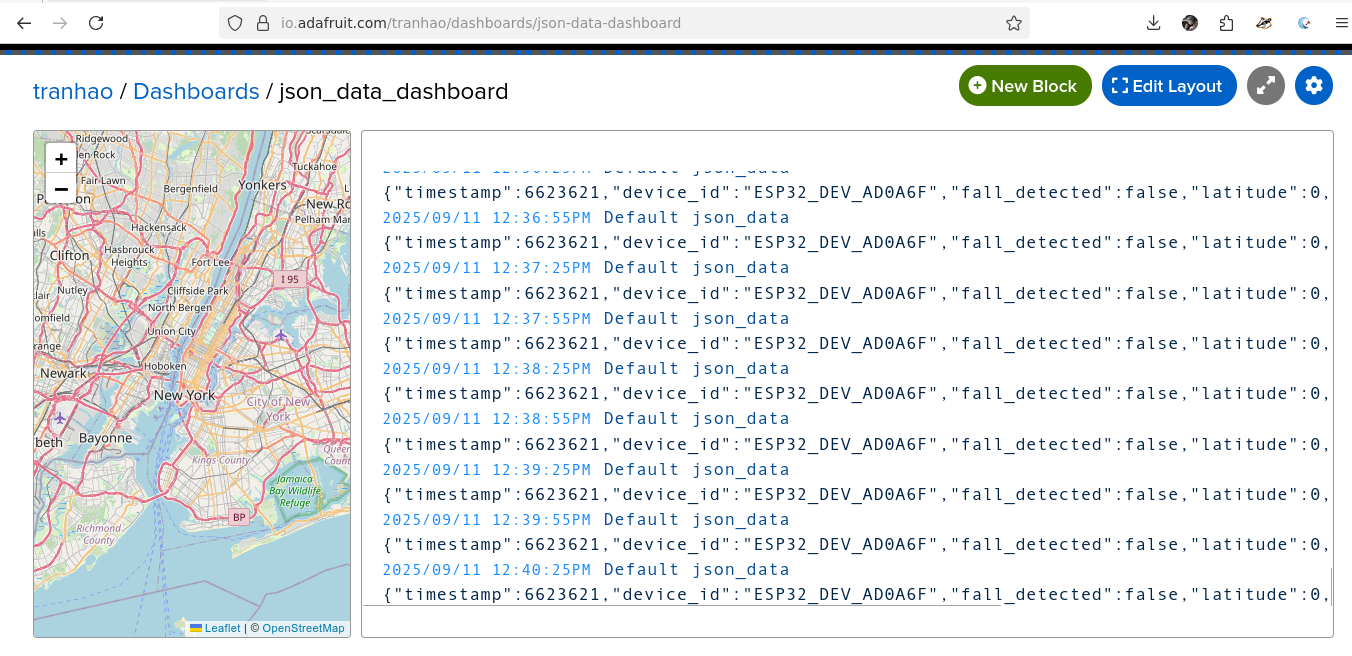
\includegraphics[width=0.8\textwidth]{figures/json_data_dashboard.png}
    \caption{Dashboard hiển thị bản tin MQTT từ thiết bị ESP32.}
    \label{fig:mqtt_dashboard}
\end{figure}

\textit{Kết luận:} Kết nối MQTT ổn định, đảm bảo thiết bị có thể truyền dữ liệu định kỳ tới hệ thống giám sát trung tâm.

\subsection{Phát hiện té ngã và xử lý cảnh báo}
Thuật toán phát hiện ghi nhận chuỗi trạng thái từ \texttt{LOW\_G} sang \texttt{HIGH\_G}, sau đó xác nhận va chạm và kích hoạt cảnh báo.  
Cảnh báo bao gồm gửi SMS, publish bản tin MQTT, đồng thời kích hoạt buzzer và LED cục bộ.  

\begin{minted}[fontsize=\footnotesize,breaklines]{text}
E (159131) FALL_LOGIC: FALL DETECTED! Accel: 0.99 g
I (159151) SIM4G_GPS: SMS request queued successfully
I (159191) SIM4G_GPS: MQTT alert published successfully.
I (159221) buzzer: Beeping for 8000 ms
I (159881) SIM4G_AT: SMS sent successfully.
I (175241) EVENT_HANDLER: Alert sequence completed.
\end{minted}

\begin{figure}[H]
    \centering
    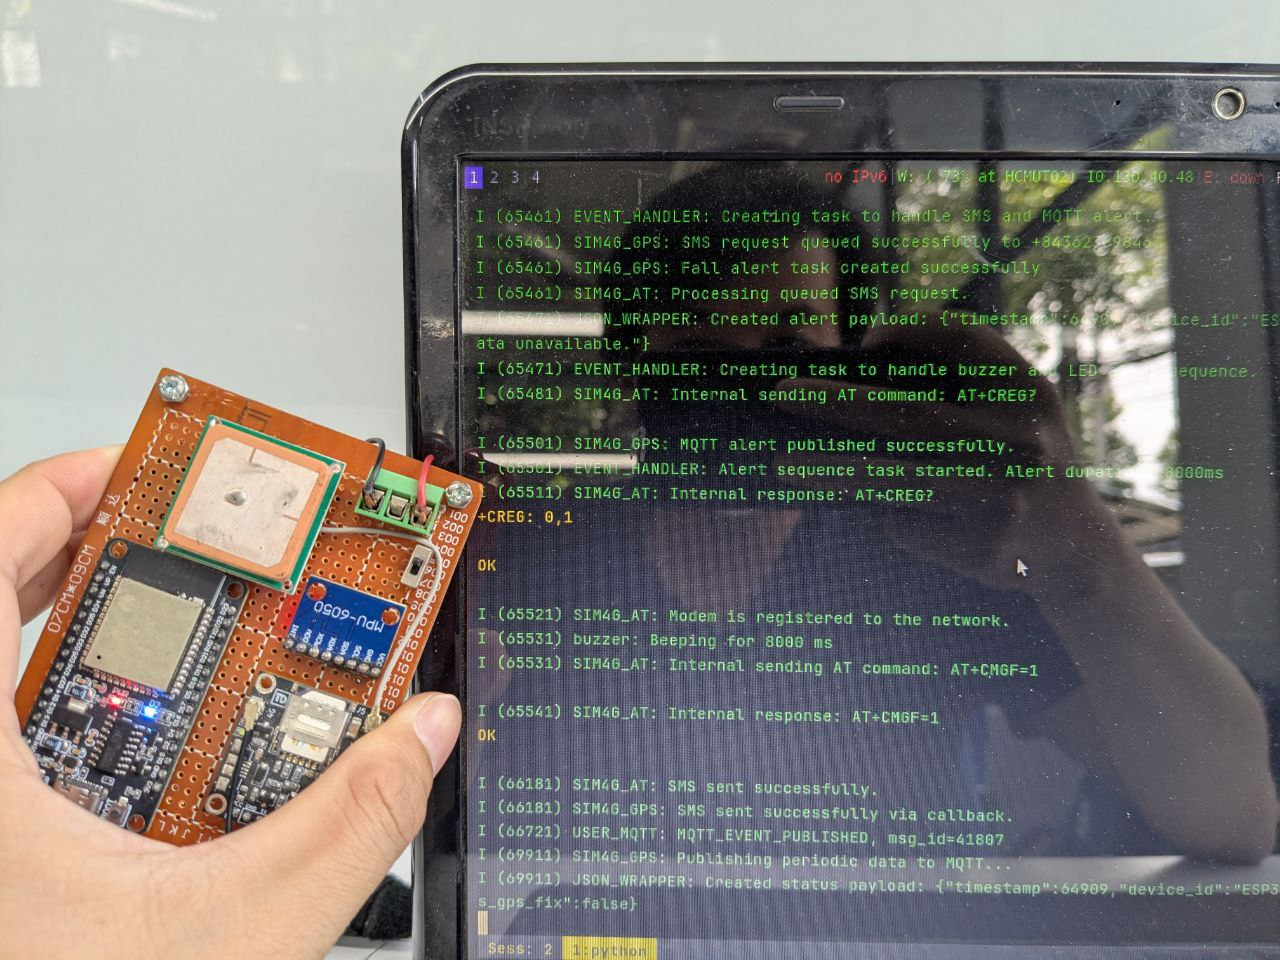
\includegraphics[width=0.8\textwidth]{figures/module1_real_log.jpg}
    \caption{Log thực tế của module cảm biến đeo khi phát hiện té ngã và kích hoạt cảnh báo.}
    \label{fig:module1_real_log}
\end{figure}

\textit{Kết luận:} Hệ thống phát hiện và xử lý cảnh báo té ngã thành công, kích hoạt đồng thời nhiều kênh cảnh báo.

\subsection{Module Camera và truyền hình ảnh}
Module ESP32-CAM được kiểm tra để xác nhận khả năng kết nối Wi-Fi và phát luồng hình ảnh qua HTTP.  
Kết quả log cho thấy camera được nhận diện đúng (OV5640), server HTTP đã khởi động và tốc độ khung hình trung bình dao động trong khoảng 3.5–5 FPS.
\begin{figure}[H]
    \centering
    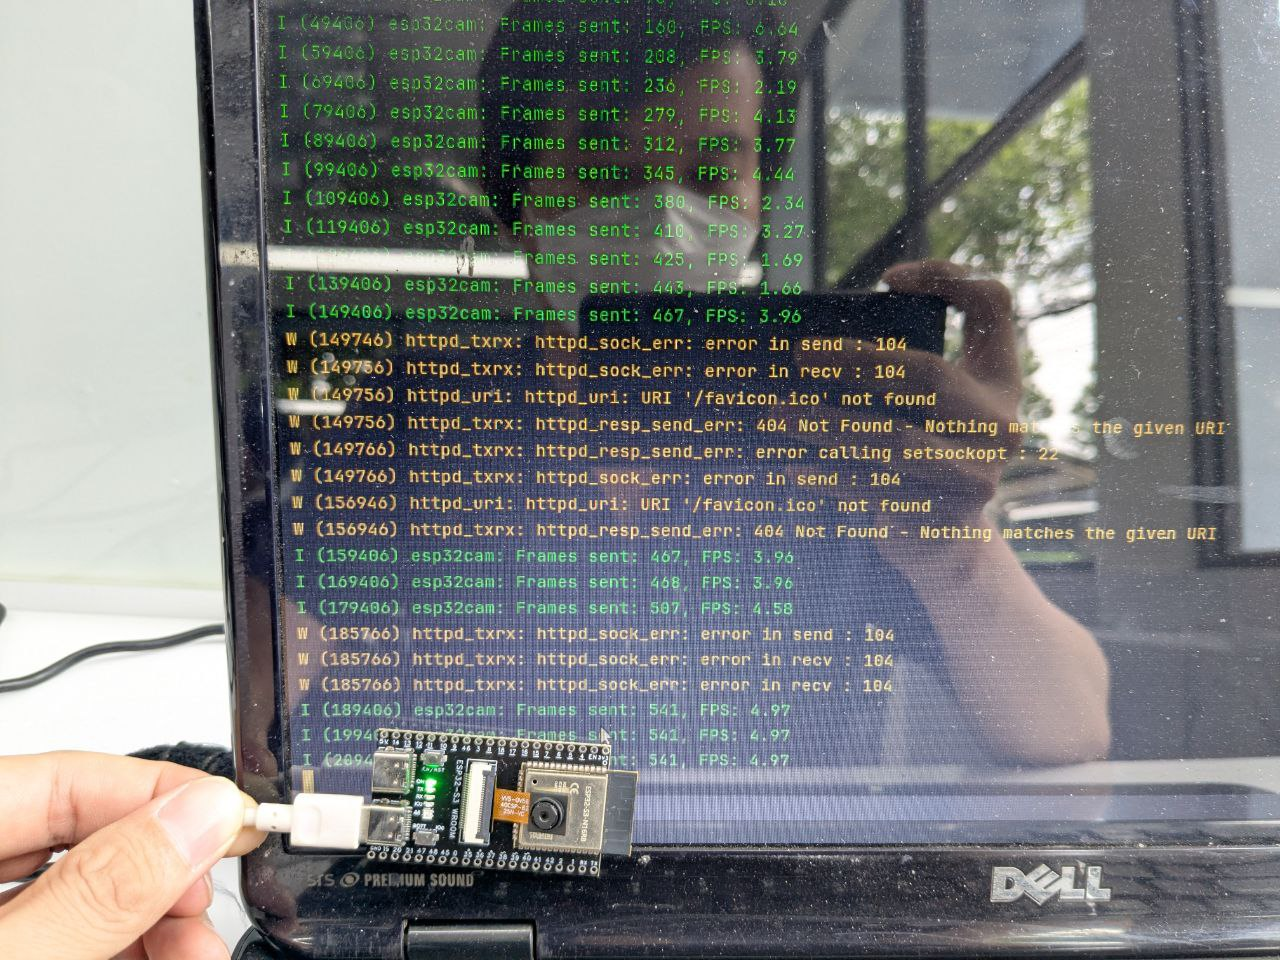
\includegraphics[width=0.8\textwidth]{figures/module2_real_log.jpg}
    \caption{Log thực tế của module esp-camera.}
    \label{fig:module2_real_log}
\end{figure}


\begin{minted}[fontsize=\footnotesize,breaklines]{text}
I (8936) esp32cam: Got IP: 10.110.87.85
I (9266) camera: Detected OV5640 camera
I (10006) esp32cam: HTTP server started
I (20006) esp32cam: Frames sent: 50, FPS: 5.87
I (40006) esp32cam: Frames sent: 146, FPS: 4.46
\end{minted}

\begin{figure}[H]
    \centering
    
\includegraphics[width=0.8\textwidth]{figures/module2_stream_example.jpg}
    \caption{Luồng hình ảnh phát từ module ESP32-CAM qua HTTP.}
    \label{fig:camera_stream}
\end{figure}

\textit{Kết luận:} Module camera hoạt động ổn định, cho phép giám sát hình ảnh trực tiếp phục vụ xác minh sự kiện té ngã.

\subsection{Kiểm tra Xử lý nhận diện hình ảnh (Python)}
Module xử lý hình ảnh bằng Python nhận luồng video từ camera ESP32-CAM hoặc webcam, sau đó sử dụng TensorFlow Lite để phát hiện người và trích xuất các điểm khớp (skeleton) theo thời gian thực.  

Quy trình xử lý bao gồm:
\begin{itemize}
    \item Khởi tạo pipeline nhận luồng video từ camera.  
    \item Tiền xử lý khung hình (chuẩn hóa kích thước, màu sắc).  
    \item Chạy mô hình học máy TensorFlow Lite để phát hiện và trích xuất các điểm khớp của cơ thể người.  
    \item Vẽ skeleton trực quan trên khung hình để theo dõi trạng thái và chuyển động.  
\end{itemize}

Kết quả thực nghiệm cho thấy module hoạt động ổn định, xử lý khung hình theo thời gian thực với tốc độ trung bình 3--5 FPS.  
Hình~\ref{fig:python_skeleton} minh họa giao diện theo dõi người và skeleton được module xử lý hình ảnh tạo ra trong quá trình chạy thử nghiệm.

\begin{figure}[H]
    \centering
    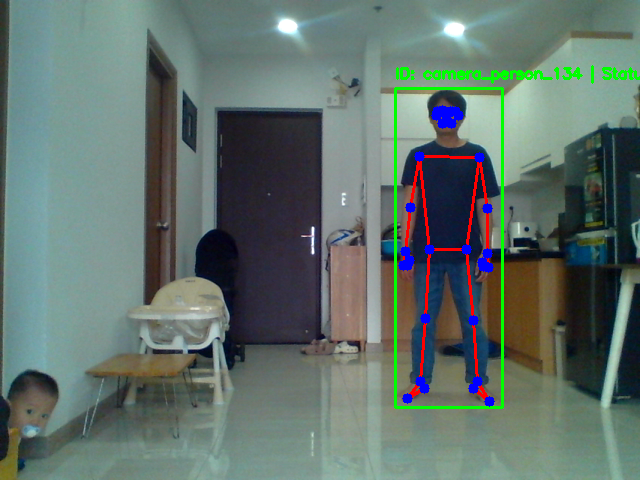
\includegraphics[width=0.85\textwidth]{figures/fall_detection_screen_shoot.png}
    \caption{Module Python xử lý hình ảnh: phát hiện người và vẽ skeleton theo thời gian thực.}
    \label{fig:python_skeleton}
\end{figure}


Module máy chủ xử lý được xây dựng bằng Python nhằm thực hiện các chức năng: thu nhận luồng dữ liệu từ camera, triển khai mô hình học sâu để dựng khung xương (skeleton), đồng thời tích hợp với hệ thống gửi cảnh báo qua MQTT và Telegram. Ngoài ra, module còn ghi log vào cơ sở dữ liệu SQLite và duy trì kết nối với Asterisk Management Interface (AMI).  

\begin{figure}[H]
    \centering
    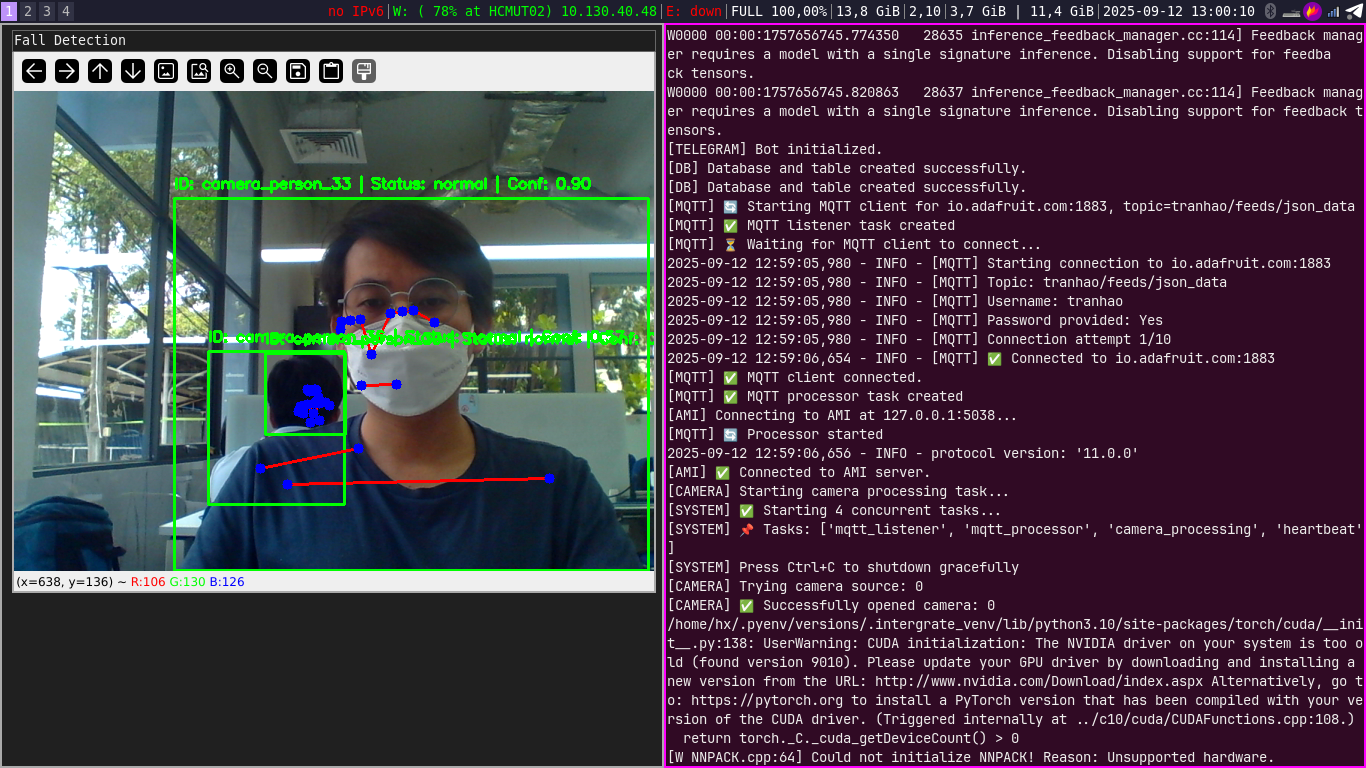
\includegraphics[width=0.8\textwidth]{figures/python_runing_log.png}
    \caption{Log thực nghiệm: Python xử lý ảnh và điều phối các tác vụ.}
    \label{fig:python_runing_log}
\end{figure}

\textbf{Kết luận:} Module Python đã hoạt động đúng chức năng, bảo đảm khả năng thu nhận dữ liệu camera, chạy nhận diện hình ảnh, đồng bộ dữ liệu qua MQTT, và kích hoạt các kênh cảnh báo. Hệ thống tuy có hạn chế về hỗ trợ CUDA (do phiên bản driver cũ) nhưng không ảnh hưởng đến quá trình thực thi trên CPU.

\subsection{Đánh giá thực nghiệm cảm biến mpu,gps và dữ liệu thu thập}
\subsubsection*{Quy trình thử nghiệm}
Để đánh giá hiệu quả hoạt động của hệ thống trong thực tế, quy trình thử nghiệm được tiến hành theo các bước:
\begin{enumerate}
    \item Nạp chương trình vào ESP32 bằng \texttt{idf.py flash monitor}.  
    \item Giả lập tình huống té ngã bằng cách lắc mạnh hoặc thả nhẹ thiết bị.  
    \item Quan sát log hệ thống để xác nhận sự kiện.  
    \item Kiểm tra tính năng gửi cảnh báo SMS với dữ liệu GPS.  
\end{enumerate}

\subsubsection*{Phân tích dữ liệu cảm biến}
Trong quá trình thử nghiệm, dữ liệu MPU6050 được thu thập cho hai trạng thái: \textbf{té ngã} và \textbf{bình thường}.  
Các bảng dưới đây trình bày dữ liệu đã ghi nhận.


\begin{table}[H]
\centering
\caption{Dữ liệu MPU6050 trong trạng thái té ngã}
\label{tab:fall_log_data}
\begin{tabular}{|c|c|c|c|c|c|c|}
\hline
\textbf{Time (ms)} & \textbf{Accel X (g)} & \textbf{Accel Y (g)} & \textbf{Accel Z (g)} & \textbf{Gyro X (dps)} & \textbf{Gyro Y (dps)} & \textbf{Gyro Z (dps)} \\
\hline
10338 & 0.06 & -0.12 & -1.00 & -22.50 & 47.18 & -77.85 \\
12338 & 0.20 & -0.09 & -0.96 & -79.74 & -64.79 & 22.34 \\
16338 & 0.10 & 0.02  & -1.19 & 23.37  & 14.82  & -4.84 \\
17338 & -0.25 & -0.13 & -0.82 & -42.96 & -8.53  & 18.43 \\
20338 & 0.18 & 0.07  & -1.02 & -50.80 & 32.41  & 15.31 \\
26338 & -1.56 & 1.06  & -2.00 & 168.47 & 250.13 & 116.60 \\
29338 & -2.00 & -1.69 & -1.29 & 250.13 & 250.13 & 38.65 \\
43338 & 0.33 & 0.07  & 0.23  & -157.85 & -61.94 & -188.73 \\
\hline
\end{tabular}
\end{table}

\begin{table}[H]
\centering
\caption{Dữ liệu MPU6050 trong trạng thái bình thường}
\label{tab:normal_log_data}
\begin{tabular}{|c|c|c|c|c|c|c|}
\hline
\textbf{Time (ms)} & \textbf{Accel X (g)} & \textbf{Accel Y (g)} & \textbf{Accel Z (g)} & \textbf{Gyro X (dps)} & \textbf{Gyro Y (dps)} & \textbf{Gyro Z (dps)} \\
\hline
328  & -0.19 & -0.22 & -0.93 & 1.08 & -1.18 & 0.38 \\
1338 & -0.19 & -0.22 & -0.93 & 1.03 & -1.38 & 0.64 \\
2338 & -0.20 & -0.22 & -0.94 & 1.19 & -1.13 & 0.18 \\
3338 & -0.19 & -0.22 & -0.93 & 1.07 & -0.95 & 0.35 \\
4338 & -0.19 & -0.22 & -0.93 & 0.99 & -1.02 & -0.02 \\
5338 & -0.19 & -0.22 & -0.94 & 1.18 & -1.33 & 0.29 \\
6338 & -0.19 & -0.22 & -0.93 & 0.95 & -1.42 & 0.21 \\
\hline
\end{tabular}
\end{table}
% Bảng so sánh

\begin{table}[H]
\centering
\caption{So sánh đặc trưng dữ liệu MPU6050 giữa trạng thái bình thường và té ngã}
\label{tab:mpu6050_new_comparison}
\begin{tabular}{|l|c|c|p{7cm}|}
\hline
\textbf{Thông số} & \textbf{Bình thường} & \textbf{Té ngã} & \textbf{Nhận xét và ý nghĩa} \\
\hline
Biên độ Gyro (X,Y,Z) & $\pm 1.5$ dps & $\pm 250$ dps & Té ngã làm dao động góc tăng vọt, nhiều lần đạt cực trị giới hạn cảm biến. \\
\hline
Độ lớn Accel (XYZ) & $\approx -0.93$ g ổn định & dao động từ $-2.0$ g đến $+1.0$ g & Trạng thái bình thường chỉ phản ánh trọng lực, trong khi té ngã tạo biến thiên mạnh ở nhiều trục. \\
\hline
Độ lớn Gyro (Mag) & 1 -- 2 dps & 100 -- 400 dps & Rõ rệt sự khác biệt, té ngã gây xoay mạnh. \\
\hline
Độ lớn Accel (Mag) & 0.95 -- 0.97 g & 0.7 -- 2.0 g & Té ngã làm gia tốc tổng hợp vượt khỏi mức tĩnh, thể hiện xung lực va chạm. \\
\hline
\end{tabular}
\end{table}

\begin{table}[H]
\centering
\caption{Dữ liệu vector (gia tốc và con quay hồi chuyển) theo ba trạng thái}
\label{tab:vector_data}
\begin{tabular}{|c|c|c|c|}
\hline
\textbf{Time (ms)} & \textbf{Accel\_Mag (g)} & \textbf{Gyro\_Mag (dps)} & \textbf{State} \\
\hline
328   & 0.99 & 1.66 & Normal \\
1338  & 1.01 & 1.77 & Normal \\
2338  & 1.02 & 1.70 & Normal \\
9338  & 1.05 & 5.80 & Fall \\
9438  & 1.27 & 5.77 & Fall \\
9538  & 1.21 & 5.90 & Fall \\
10338 & 1.00 & 0.25 & Post-Fall \\
11338 & 1.02 & 0.09 & Post-Fall \\
12338 & 1.01 & 0.15 & Post-Fall \\
\hline
\end{tabular}
\end{table}

\begin{figure}[H]
    \centering
    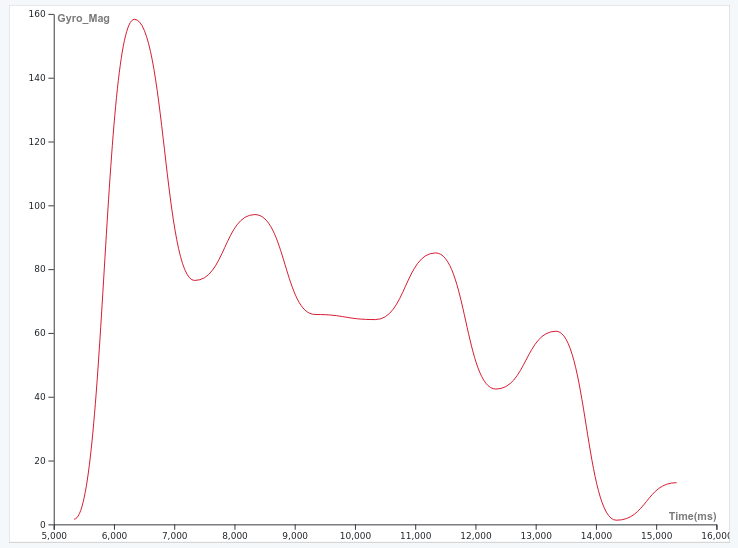
\includegraphics[width=0.95\linewidth]{figures/gyro_time.png}
    \caption{Biến thiên magnitude của gia tốc góc (Gyro\_Mag) theo thời gian.}
    \label{fig:gyro_time}
\end{figure}

\paragraph{Miêu tả và phân tích (Gyro theo thời gian).}
Đồ thị \ref{fig:gyro_time} biểu diễn biến thiên của đại lượng \texttt{Gyro\_Mag} (magnitude của vector con quay hồi chuyển) theo mốc thời gian thử nghiệm. Đồ thị thể hiện rõ ba pha hoạt động: 
\begin{itemize}
  \item \textbf{Bình thường (Normal):} \texttt{Gyro\_Mag} dao động rất nhỏ quanh giá trị nền (thường $\lesssim 2$ dps), biểu thị chuyển động góc nhẹ hoặc ổn định khi đeo thiết bị.
  \item \textbf{Sự kiện té ngã (Fall):} tại thời điểm xảy ra té, xuất hiện đỉnh đột biến lớn (thường tăng lên hàng chục đến hàng trăm dps). Các đỉnh này là đặc trưng nhận diện sự xoay mạnh và va chạm trong pha té.
  \item \textbf{Hậu té (Post-Fall):} sau đỉnh, \texttt{Gyro\_Mag} giảm nhanh về mức nền hoặc gần không, thể hiện trạng thái nằm yên và thiếu chuyển động góc.
\end{itemize}

Những quan sát quan trọng rút ra từ đồ thị:
\begin{enumerate}
  \item Biên độ đỉnh \texttt{Gyro\_Mag} trong pha \textit{Fall} lớn hơn nhiều so với dao động nền — hiệu quả để làm ngưỡng phân loại (ví dụ threshold tạm ứng: $>20$--$50$ dps tùy thực nghiệm).
  \item Hình thái thời gian của đỉnh (rise time và decay) cho phép phân biệt giữa cú va chạm thực sự và nhiễu ngắn (spike): cú té thật thường có đỉnh rộng hơn và kèm biến động phụ ở các trục.
\end{enumerate}

\vspace{6pt}

\begin{figure}[H]
    \centering
    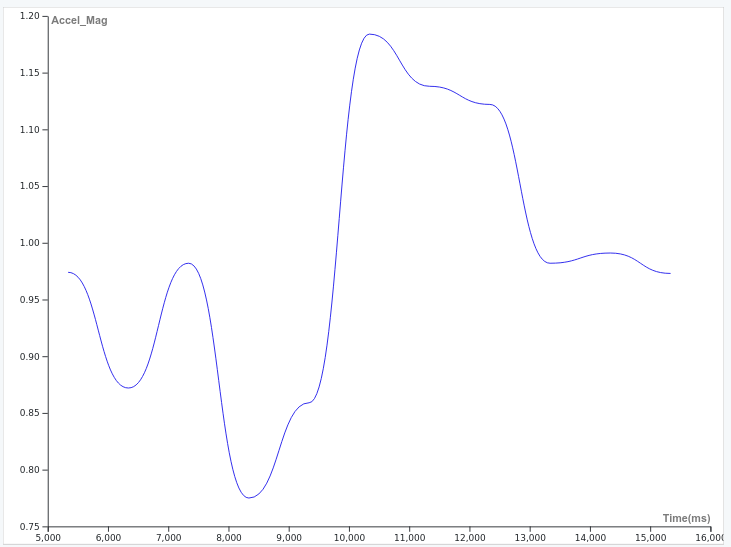
\includegraphics[width=0.95\linewidth]{figures/accel_time.png}
    \caption{Biến thiên magnitude của gia tốc (Accel\_Mag) theo thời gian.}
    \label{fig:accel_time}
\end{figure}

\paragraph{Miêu tả và phân tích (Accel theo thời gian).}
Đồ thị \ref{fig:accel_time} trình bày biến thiên \texttt{Accel\_Mag} (magnitude của vector gia tốc) theo cùng mốc thời gian. Diễn biến cũng chia làm ba pha tương tự:
\begin{itemize}
  \item \textbf{Bình thường (Normal):} \texttt{Accel\_Mag} nằm gần 1\,g (do trọng lực), dao động nhẹ quanh giá trị này khi người vận động nhẹ.
  \item \textbf{Sự kiện té ngã (Fall):} \texttt{Accel\_Mag} xuất hiện các xung hoặc thay đổi đột ngột, có thể vượt hoặc giảm mạnh so với 1\,g (tùy hướng va chạm), đặc biệt khi có va chạm mạnh xung lực tổng hợp có xu hướng lớn hơn 1\,g đáng kể.
  \item \textbf{Hậu té (Post-Fall):} \texttt{Accel\_Mag} trở về gần 1\,g nhưng với phân bố vector (các thành phần X/Y/Z) có thể đổi hướng so với trạng thái trước té (chỉ ra tư thế nằm).
\end{itemize}

\begin{enumerate}
  \item Sự tăng/giảm đột ngột của \texttt{Accel\_Mag} là chỉ báo trực tiếp của xung lực trong sự kiện té; phối hợp với \texttt{Gyro\_Mag} giúp loại bỏ nhiễu giả   \item Dao động nền quanh 1\,g cho phép hiệu chuẩn nhanh: mọi giá trị lệch bền khỏi 1\,g trong một khoảng thời gian ngắn.
\end{enumerate}

\textit{Kết luận:} Dữ liệu cảm biến cho thấy sự khác biệt rõ rệt giữa hai trạng thái. Đặc biệt, \textbf{Accel Mag} và \textbf{Gyro Mag} là chỉ báo hiệu quả để phát hiện té ngã, cung cấp cơ sở thực nghiệm cho việc tinh chỉnh ngưỡng phát hiện và giảm thiểu cảnh báo sai.

\begin{table}[H]
\centering
\caption{Bảng kết quả thu được từ log test của mô-đun 4G/GPS}
\label{tab:gps_data}
\begin{tabular}{|c|c|c|c|c|c|c|}
\hline
\textbf{Time (UTC)} & \textbf{Latitude} & \textbf{Longitude} & \textbf{Altitude (m)} & \textbf{Fix Mode} & \textbf{Date} & \textbf{Satellites} \\
\hline
132517.00 & 1053.3115N & 10646.7839E & 5.07 & 3 & 240425 & 07 \\
132517.00 & 1053.3115N & 10646.7839E & 5.07 & 3 & 240425 & 07 \\
132540.00 & 1053.3117N & 10646.7840E & 5.05 & 3 & 240425 & 07 \\
132540.00 & 1053.3117N & 10646.7840E & 5.05 & 3 & 240425 & 07 \\
132627.00 & 1053.3107N & 10646.7839E & 5.02 & 3 & 240425 & 07 \\
132627.00 & 1053.3107N & 10646.7839E & 5.02 & 3 & 240425 & 07 \\
\hline
\end{tabular}
\end{table}
% Bảng dữ liệu té ngã
% Bảng dữ liệu bình thường
% Bảng dữ liệu GPS

\begin{table}[H]
\centering
\caption{Phân tích và giải thích dữ liệu GPS thu được}
\label{tab:gps_analysis}
\begin{tabular}{|l|c|p{8.5cm}|}
\hline
\textbf{Trường dữ liệu} & \textbf{Giá trị điển hình} & \textbf{Giải thích và ý nghĩa} \\
\hline
Thời gian (UTC) & 132517.00 -- 132627.00 & Dữ liệu được ghi nhận liên tục trong khoảng 1 phút; cho thấy tín hiệu GPS ổn định và không bị gián đoạn. \\
\hline
Vĩ độ (Latitude) & 10°53.3115'N & Vị trí xác định chính xác đến phần giây thập phân, phù hợp với khu vực thử nghiệm thực tế. \\
\hline
Kinh độ (Longitude) & 106°46.7839'E & Giá trị duy trì ổn định qua nhiều lần đo; chứng tỏ tín hiệu ít nhiễu và đáng tin cậy. \\
\hline
Độ cao (Altitude) & $\approx 5$ m & Độ cao phản ánh đúng địa hình khu vực thử nghiệm, dao động rất nhỏ (±0.05 m). \\
\hline
Chế độ định vị (Fix Mode) & 3 & Chế độ định vị 3D, đảm bảo độ chính xác cao khi xác định cả vĩ độ, kinh độ và độ cao. \\
\hline
Ngày (Date) & 24/04/2025 & Thời điểm dữ liệu được ghi nhận, khớp với lịch trình thử nghiệm. \\
\hline
Số vệ tinh (Satellites) & 07 & Số vệ tinh thu được đủ lớn để đảm bảo tín hiệu ổn định, độ tin cậy cao trong định vị. \\
\hline
\end{tabular}
\end{table}

\subsection{Kết quả thử nghiệm chức năng gọi và nhắn tin cảnh báo qua Asterisk AMI}
\label{subsec:ast_call_sms_test}

Để kiểm chứng khả năng kích hoạt cảnh báo tự động qua tổng đài Asterisk, hệ thống đã được cấu hình thực hiện đồng thời cuộc gọi và gửi tin nhắn SMS đến ba extension (\texttt{6001}, \texttt{6002}, \texttt{6003}). Kết quả log thử nghiệm được thể hiện trong Hình~\ref{fig:ast_call_sms_test}.

Như quan sát trên log, quá trình kết nối tới Asterisk AMI được thực hiện thành công và hệ thống đã gửi tin nhắn đến các extension. Tin nhắn SMS tới \texttt{6001} và \texttt{6002} được gửi thành công, trong khi SMS tới \texttt{6003} gặp lỗi truyền tải. Ngoài ra, các dòng báo lỗi cuối cùng liên quan tới thao tác gọi điện xuất hiện do hệ thống chỉ kích hoạt cuộc gọi báo động mà không có nội dung thoại kèm theo. Việc này dẫn đến ngoại lệ \texttt{'list' object has no attribute 'get'}, nhưng không ảnh hưởng tới cơ chế gửi cảnh báo chính.

\begin{figure}[H]
    \centering
    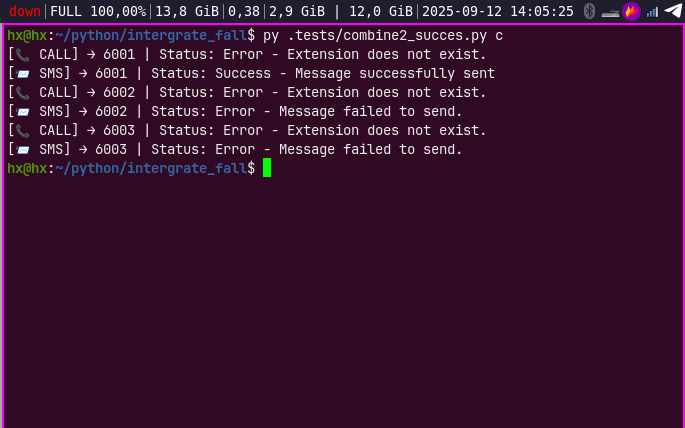
\includegraphics[width=0.95\linewidth]{figures/ast_call_sms_test.png}
    \caption{Kết quả thử nghiệm chức năng gọi và nhắn tin cảnh báo qua Asterisk AMI}
    \label{fig:ast_call_sms_test}
\end{figure}

\textit{Kết luận:}Kết quả thử nghiệm cho thấy hệ thống có thể gửi cảnh báo qua cuộc gọi và SMS thành công tới các extension, ngoại trừ một số lỗi ngoại lệ khi gọi điện do không có nội dung thoại, nhưng điều này không ảnh hưởng đến chức năng cảnh báo chính, chứng minh khả năng hoạt động theo đúng ý định ban đầu.

\subsection{Thử nghiệm Kênh cảnh báo Telegram}
\label{sec:telegram_alert}

Hệ thống Telegram Bot đóng vai trò là kênh cảnh báo trực quan, giúp gửi thông báo đến người dùng ngay khi phát hiện té ngã.  
Cơ chế hoạt động được chia thành hai hướng:
\begin{itemize}
    \item \textbf{Từ module phần cứng (ESP32 + 4G/GPS):} Khi xảy ra sự kiện té ngã, bản tin MQTT được phát ra từ thiết bị. Hệ thống trung tâm chuyển tiếp xử lý nội dung này đến người dùng thông qua Telegram.
    \item \textbf{Từ module xử lý hình ảnh (Python):} Khi nhận diện được té ngã qua camera và skeleton, hệ thống Python trực tiếp gửi cảnh báo đến Telegram, kèm thông tin chi tiết về hình chụp từ camera và tin nhắn kèm theo.
\end{itemize}

\begin{figure}[H]
    \centering
    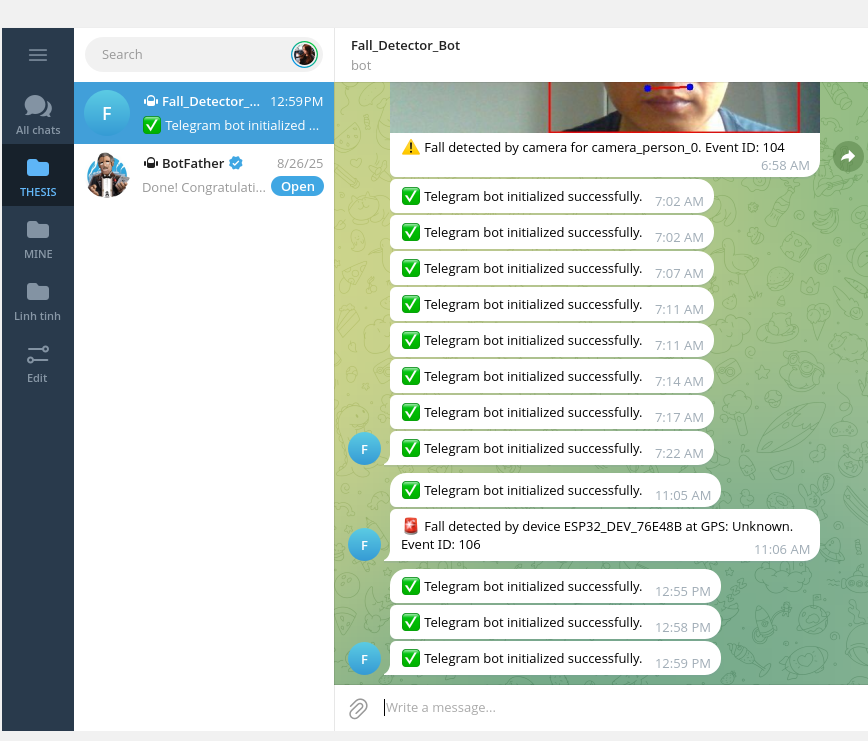
\includegraphics[width=0.8\textwidth]{figures/telegram_fall_module1_send.png}
    \caption{Thông báo cảnh báo té ngã từ module phần cứng (ESP32) qua Telegram.}
    \label{fig:telegram_hw}
\end{figure}

\begin{figure}[H]
    \centering
    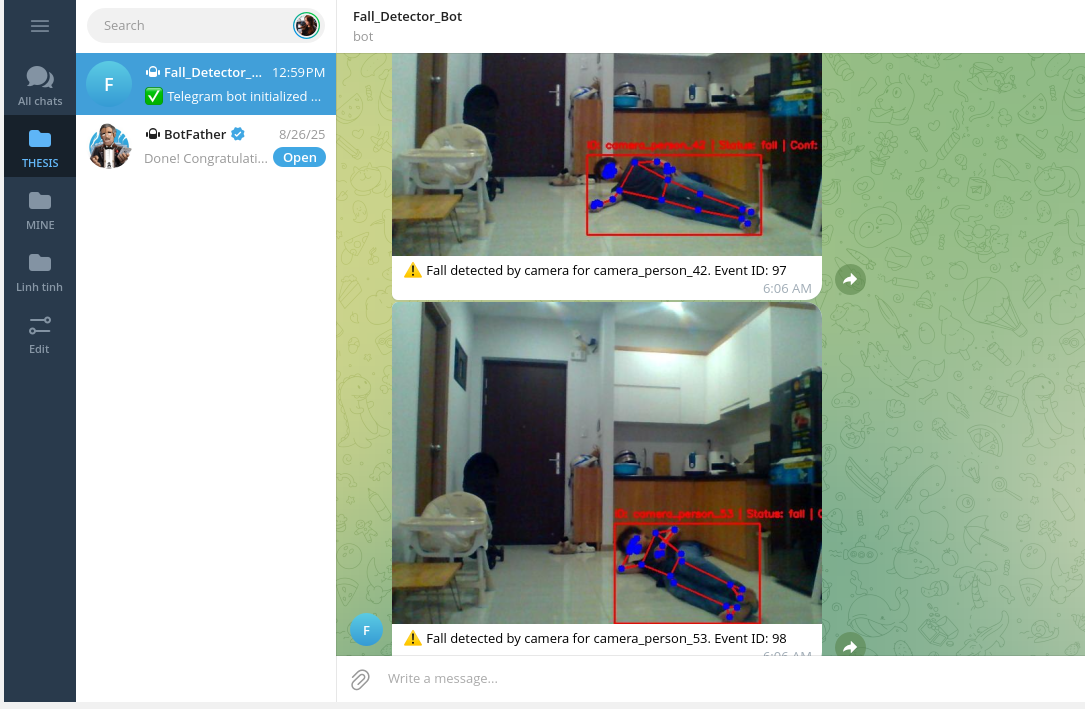
\includegraphics[width=0.8\textwidth]{figures/telegram_python_fall_send.png}
    \caption{Thông báo cảnh báo té ngã từ module xử lý hình ảnh Python qua Telegram.}
    \label{fig:telegram_python}
\end{figure}

\textit{Kết luận:} Kênh Telegram đã hoạt động ổn định, đóng vai trò cầu nối giữa hệ thống phát hiện té ngã và người dùng cuối. Việc kết hợp cả hai nguồn cảnh báo (thiết bị phần cứng và module xử lý hình ảnh) giúp tăng độ tin cậy và giảm thiểu khả năng bỏ sót sự kiện.
 % 4.2 Fall detection performance (Accuracy, Sensitivity)


\subsection{Xử lý hình ảnh Python}
Module xử lý hình ảnh bằng Python nhận luồng video từ camera ESP32-CAM hoặc webcam, sau đó sử dụng TensorFlow Lite để phát hiện người và trích xuất các điểm khớp (skeleton) theo thời gian thực.  

Quy trình xử lý bao gồm:
\begin{itemize}
    \item Khởi tạo pipeline nhận luồng video từ camera.  
    \item Tiền xử lý khung hình (chuẩn hóa kích thước, màu sắc).  
    \item Chạy mô hình học máy TensorFlow Lite để phát hiện và trích xuất các điểm khớp của cơ thể người.  
    \item Vẽ skeleton trực quan trên khung hình để theo dõi trạng thái và chuyển động.  
\end{itemize}

Kết quả thực nghiệm cho thấy module hoạt động ổn định, xử lý khung hình theo thời gian thực với tốc độ trung bình 3--5 FPS.  
Hình~\ref{fig:python_skeleton} minh họa giao diện theo dõi người và skeleton được module xử lý hình ảnh tạo ra trong quá trình chạy thử nghiệm.

\begin{figure}[H]
    \centering
    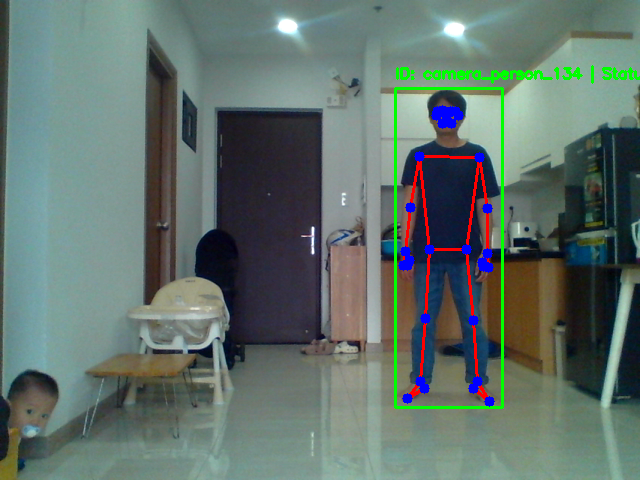
\includegraphics[width=0.85\textwidth]{figures/fall_detection_screen_shoot.png}
    \caption{Module Python xử lý hình ảnh: phát hiện người và vẽ skeleton theo thời gian thực.}
    \label{fig:python_skeleton}
\end{figure}
\subsection{Module nhận diện hình ảnh (Python)}
\label{sec:python_vision}

Module máy chủ xử lý được xây dựng bằng Python nhằm thực hiện các chức năng: thu nhận luồng dữ liệu từ camera, triển khai mô hình học sâu để dựng khung xương (skeleton), đồng thời tích hợp với hệ thống gửi cảnh báo qua MQTT và Telegram. Ngoài ra, module còn ghi log vào cơ sở dữ liệu SQLite và duy trì kết nối với Asterisk Management Interface (AMI).  

\begin{figure}[H]
    \centering
    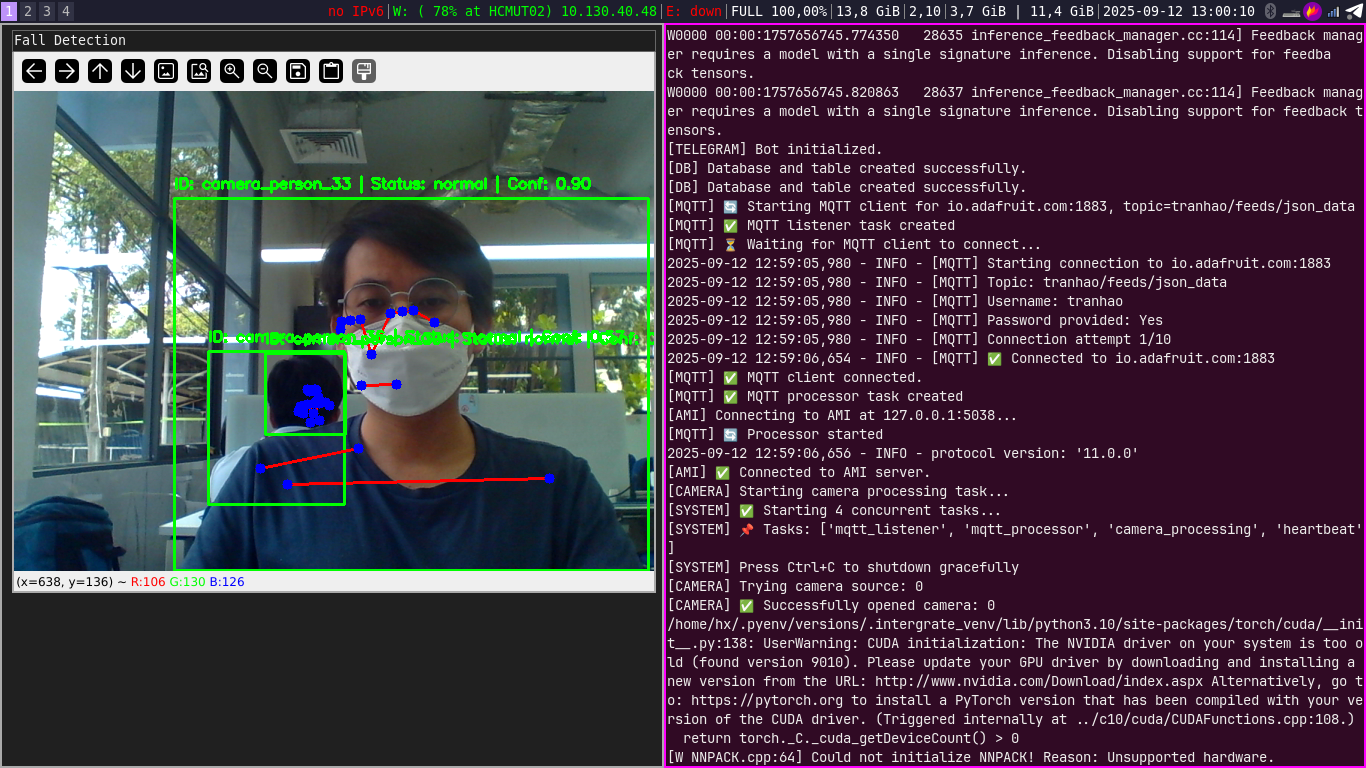
\includegraphics[width=0.8\textwidth]{figures/python_runing_log.png}
    \caption{Log thực nghiệm: Python xử lý ảnh và điều phối các tác vụ.}
    \label{fig:python_runing_log}
\end{figure}

\textbf{Kết luận:} Module Python đã hoạt động đúng chức năng, bảo đảm khả năng thu nhận dữ liệu camera, chạy nhận diện hình ảnh, đồng bộ dữ liệu qua MQTT, và kích hoạt các kênh cảnh báo. Hệ thống tuy có hạn chế về hỗ trợ CUDA (do phiên bản driver cũ) nhưng không ảnh hưởng đến quá trình thực thi trên CPU.

\subsection{Thử nghiệm Asterisk Call/SMS Gateway}
\label{sec:asterisk_test}

Trong hệ thống, Asterisk được sử dụng như một cổng trung gian để gửi cảnh báo bằng SMS và có tiềm năng mở rộng sang chức năng gọi điện tự động.  
Trong quá trình thử nghiệm, việc kích hoạt nhắn tin SMS qua Asterisk hoạt động thành công, cho phép hệ thống gửi cảnh báo đến số điện thoại đã đăng ký.  

Tuy nhiên, chức năng gọi thoại chưa được triển khai ổn định. Khi thay đổi máy chủ Asterisk, cấu hình giữ nguyên nhưng khả năng khởi tạo và duy trì cuộc gọi không đồng nhất. Điều này cho thấy còn tồn tại sự phụ thuộc vào môi trường triển khai, cần được nghiên cứu và tối ưu thêm trong tương lai.  

\begin{figure}[H]
    \centering
    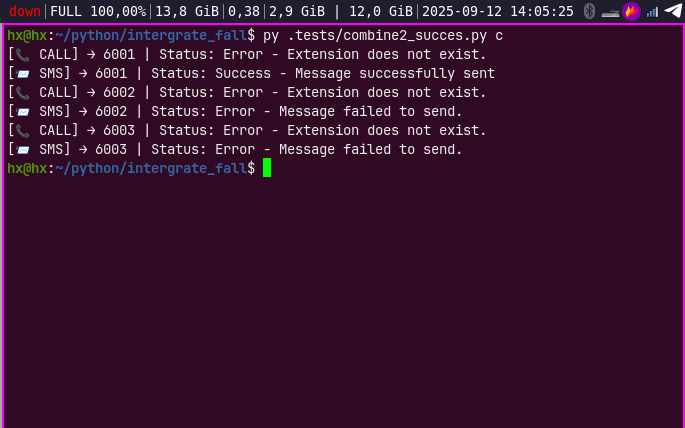
\includegraphics[width=0.8\textwidth]{figures/ast_call_sms_test.png}
    \caption{Thử nghiệm gửi SMS cảnh báo qua Asterisk.}
    \label{fig:ast_call_sms_test}
\end{figure}

\textit{Kết luận:} Module Asterisk đã hỗ trợ thành công chức năng nhắn tin SMS trong hệ thống. Chức năng gọi thoại vẫn còn hạn chế và sẽ cần nghiên cứu bổ sung để đảm bảo tính ổn định khi triển khai thực tế.

\subsection{Kênh cảnh báo Telegram}
\label{sec:telegram_alert}

Hệ thống Telegram Bot đóng vai trò là kênh cảnh báo trực quan, giúp gửi thông báo đến người dùng ngay khi phát hiện té ngã.  
Cơ chế hoạt động được chia thành hai hướng:
\begin{itemize}
    \item \textbf{Từ module phần cứng (ESP32 + 4G/GPS):} Khi xảy ra sự kiện té ngã, bản tin MQTT hoặc SMS được phát ra từ thiết bị. Hệ thống trung tâm sau đó chuyển tiếp nội dung này đến người dùng thông qua Telegram.
    \item \textbf{Từ module xử lý hình ảnh (Python):} Khi nhận diện được té ngã qua camera và skeleton, hệ thống Python trực tiếp gửi cảnh báo đến Telegram, kèm thông tin chi tiết.
\end{itemize}

\begin{figure}[H]
    \centering
    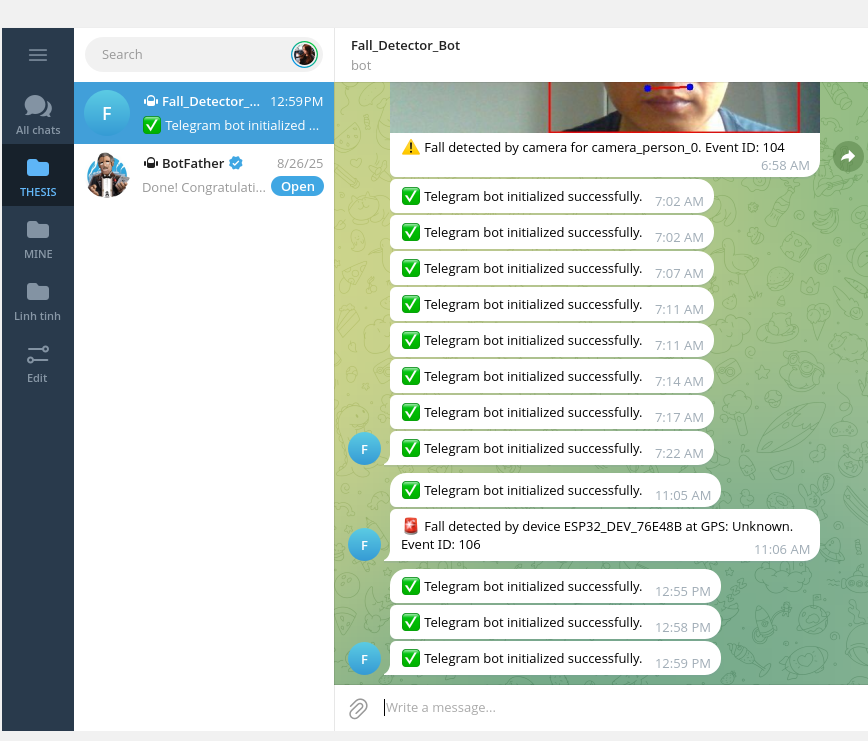
\includegraphics[width=0.8\textwidth]{figures/telegram_fall_module1_send.png}
    \caption{Thông báo cảnh báo té ngã từ module phần cứng (ESP32) qua Telegram.}
    \label{fig:telegram_hw}
\end{figure}

\begin{figure}[H]
    \centering
    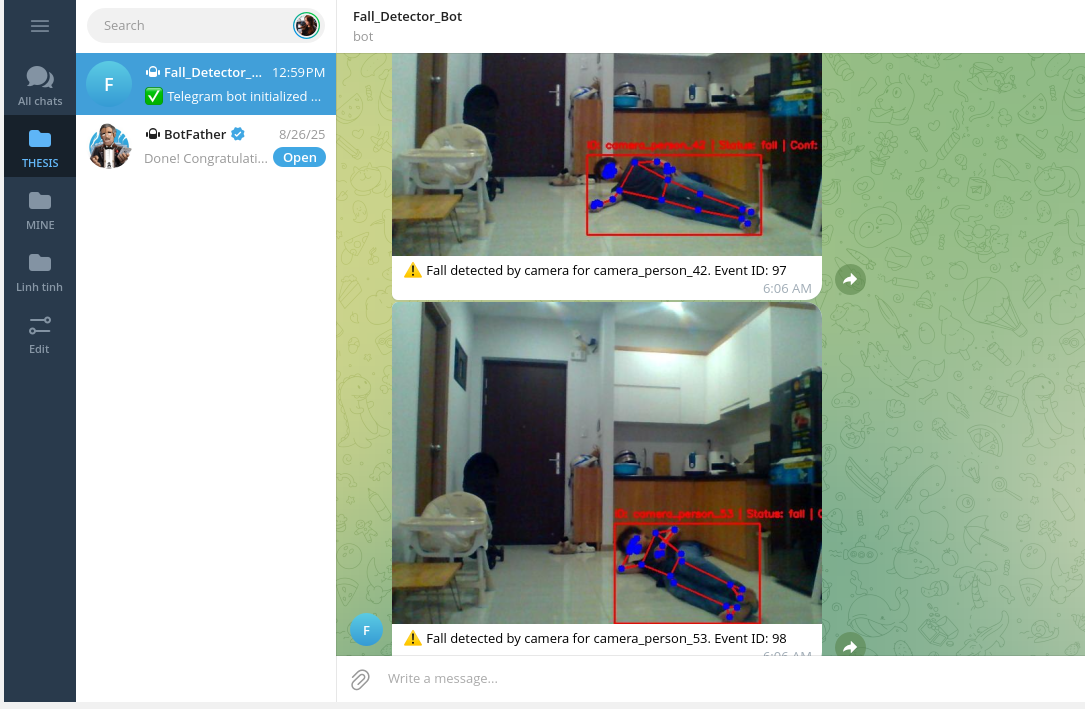
\includegraphics[width=0.8\textwidth]{figures/telegram_python_fall_send.png}
    \caption{Thông báo cảnh báo té ngã từ module xử lý hình ảnh Python qua Telegram.}
    \label{fig:telegram_python}
\end{figure}

\textit{Kết luận:} Kênh Telegram đã hoạt động ổn định, đóng vai trò cầu nối giữa hệ thống phát hiện té ngã và người dùng cuối. Việc kết hợp cả hai nguồn cảnh báo (thiết bị phần cứng và module xử lý hình ảnh) giúp tăng độ tin cậy và giảm thiểu khả năng bỏ sót sự kiện.
 % 4.3 Latency and computational efficiency
\section{Đánh giá độ ổn định}
\label{sec:stability_evaluation}

Trong quá trình thử nghiệm, thiết bị cảm biến đeo được bật liên tục và thực hiện nhiều lần mô phỏng té ngã. Thiết bị được kết nối với máy tính để theo dõi log hệ thống, từ đó giám sát các lỗi tiềm ẩn. Các vấn đề liên quan đến tràn bộ nhớ, lỗi dẫn đến watchdog reset hoặc panic hệ thống đã được xử lý trong giai đoạn phát triển. Kết quả cho thấy trong toàn bộ quá trình thử nghiệm, thiết bị hoạt động ổn định, không xuất hiện lỗi gây dừng hoặc gián đoạn hoạt động.

Song song đó, phần mềm Python được triển khai và chạy liên tục nhằm kiểm thử các chức năng của hệ thống. Nhờ việc xử lý ngoại lệ và tổ chức các module hợp lý, chương trình không xảy ra hiện tượng crash hoặc dừng đột ngột. Các luồng dữ liệu được phối hợp ổn định và chính xác trong suốt quá trình chạy. Mặc dù khi xử lý khung hình liên tục xuất hiện hiện tượng giật, lag do giới hạn hiệu năng của phần cứng máy tính, nhưng điều này không ảnh hưởng đến tính ổn định tổng thể của hệ thống.

Kết quả trên cho thấy cả thiết bị phần cứng và phần mềm điều khiển đều đạt mức ổn định cao trong điều kiện thử nghiệm liên tục, chứng minh được khả năng vận hành của hệ thống trong môi trường thực tế.

 % 4.4 Stability and reliability of the alerting system
\section{Kết luận chương}
\label{sec:chapter4_conclusion}

Trong chương này, các kết quả thực nghiệm đã được trình bày và phân tích nhằm đánh giá hiệu năng và triển khai thực tế của hệ thống phát hiện té ngã. Cụ thể: 
(i) thuật toán xử lý dữ liệu từ cảm biến MPU6050 đã chứng minh khả năng phân biệt rõ ràng giữa trạng thái bình thường và té ngã; 
(ii) độ trễ toàn hệ thống từ khi phát hiện sự kiện đến khi gửi cảnh báo đến thiết bị đầu cuối duy trì dưới 5 giây, đảm bảo yêu cầu phản hồi gần thời gian thực; 
(iii) hệ thống duy trì hoạt động ổn định trong suốt quá trình thử nghiệm, với khả năng xử lý liên tục và không xuất hiện lỗi nghiêm trọng.


 % 4.5 Chapter conclusion and discussion


\chapter{Kết luận}

Chương này tổng hợp và khái quát toàn bộ nội dung nghiên cứu trong luận văn. 
Trước hết, phần \textbf{Tóm tắt} sẽ điểm lại những kết quả chính đạt được. 
Tiếp theo, phần \textbf{Đóng góp} trình bày những điểm mới và giá trị thực tiễn của nghiên cứu. 
Phần \textbf{Hạn chế và hướng phát triển} nêu ra những điểm còn tồn tại cùng các hướng cải thiện trong tương lai. 
Cuối cùng, phần \textbf{Kết luận chung} khép lại luận văn, nhấn mạnh ý nghĩa tổng thể của công trình. 

\section{Tóm tắt kết quả thực hiện đề tài FDAS}
\label{sec:summary}

Chương này tổng hợp những kết quả trọng yếu mà luận văn đã đạt được. 
Hệ thống \textit{FDAS} dựa trên công nghệ IoT đã được xây dựng và kiểm chứng thực nghiệm. 
Các nội dung chính bao gồm:  

\begin{itemize}
    \item \textbf{Xây dựng kiến trúc hệ thống}: gồm phần cứng (ESP32, MPU6050, mô-đun SIM4G--GPS, còi cảnh báo) và phần mềm (FreeRTOS, giao tiếp UART/I\textsuperscript{2}C, MQTT, dịch vụ cảnh báo qua Telegram, Python xử lý ảnh), đảm bảo khả năng mở rộng và thích ứng với nhiều bối cảnh.
    
    \item \textbf{Phát triển thuật toán phát hiện té ngã}: 
    \begin{itemize}
        \item Dữ liệu cảm biến (gia tốc, con quay hồi chuyển) được xử lý thời gian thực trên ESP32.
        \item Dữ liệu hình ảnh/video (RGB, IR, 3D) được phân tích bằng Python để trích xuất đặc trưng và ước lượng tư thế.
        \item Kết hợp dữ liệu đa phương thức (sensor fusion) nhằm tăng độ chính xác, giảm cảnh báo giả, mở rộng tầm giám sát và phù hợp với nhiều bối cảnh khác nhau.
    \end{itemize}
    
    \item \textbf{Triển khai cơ chế cảnh báo}: sử dụng buzzer, LED, tin nhắn SMS, dịch vụ MQTT--Telegram và SIP để thông tin đến người giám sát kịp thời, bảo đảm khả năng theo dõi liên tục.
    
    \item \textbf{Thực nghiệm và kiểm chứng}: đánh giá hệ thống trong nhiều môi trường thực tế, đo lường độ chính xác phát hiện, độ trễ cảnh báo và khả năng hoạt động ổn định.
\end{itemize}

Kết quả cho thấy FDAS có tiềm năng ứng dụng cao trong giám sát sức khỏe từ xa, đặc biệt đối với người cao tuổi và bệnh nhân cần theo dõi an toàn. 
Việc tích hợp xử lý ảnh cùng dữ liệu cảm biến giúp hệ thống vừa thông minh vừa đáp ứng yêu cầu thời gian thực, nâng cao độ tin cậy so với các giải pháp đơn phương.

\section{Contribution}


\section{Hạn chế và Hướng phát triển}
\label{sec:limitation_future_work}

Mặc dù hệ thống đã chứng minh được tính khả thi, song nghiên cứu vẫn tồn tại một số hạn chế nhất định:

\begin{itemize}
    \item \textbf{Quy mô thử nghiệm còn giới hạn}: Hệ thống mới dừng ở mức kiểm chứng nguyên mẫu, chưa triển khai trên phạm vi rộng hoặc trong điều kiện thực tế đa dạng.
    \item \textbf{Số lượng thiết bị cảm biến và kênh tiếp nhận thông tin còn hạn chế}: Hệ thống chưa đủ để kiểm tra tính ổn định trong môi trường nhiều người dùng.
    \item \textbf{Thuật toán nhận diện té ngã chưa hoàn toàn ổn định}: Vẫn tồn tại khả năng xảy ra cảnh báo sai (\textit{false alarm}) hoặc bỏ sót (\textit{missed detection}).
    \item \textbf{Thiết bị đeo chưa được tối ưu}: Kích thước còn cồng kềnh, thiếu các tính năng tiện ích quan trọng như nút bấm báo khẩn cấp.
    \item \textbf{Kết nối mạng 4G chưa hoạt động hoàn chỉnh}: Mặc dù đã cấu hình được các tham số mạng nhưng chức năng truyền dữ liệu qua mạng di động vẫn chưa khai thác được.
    \item \textbf{Định vị GPS còn hạn chế}: Thiết bị có thể lấy vị trí ngoài trời, nhưng trong quá trình kích hoạt cảnh báo thực tế chưa thu thập và gửi được vị trí thành công.
\end{itemize}

Để khắc phục các hạn chế nêu trên và nâng cao khả năng ứng dụng, một số hướng phát triển được đề xuất như sau:

\begin{enumerate}
    \item \textbf{Mở rộng quy mô thử nghiệm}: Triển khai hệ thống cho nhiều người dùng, trong các bối cảnh sinh hoạt và điều kiện môi trường khác nhau để đánh giá độ tin cậy.
    \item \textbf{Cải thiện thuật toán phát hiện té ngã}: Ứng dụng các kỹ thuật học máy (\textit{machine learning}) hoặc học sâu (\textit{deep learning}) nhằm tăng độ chính xác, giảm cảnh báo sai và bỏ sót.
    \item \textbf{Tối ưu thiết bị đeo}: Thiết kế mạch phần cứng nhỏ gọn hơn, nâng cao tính tiện dụng, bổ sung nút bấm khẩn cấp hoặc cảm biến bổ trợ.
    \item \textbf{Hoàn thiện kết nối truyền thông}: Tích hợp đầy đủ chức năng kết nối 4G để đảm bảo truyền dữ liệu theo thời gian thực mà không phụ thuộc vào Wi-Fi.
    \item \textbf{Nâng cao chức năng định vị}: Tối ưu việc lấy dữ liệu GPS trong cả điều kiện ngoài trời và trong nhà (kết hợp thêm định vị Wi-Fi hoặc công nghệ khác).
    \item \textbf{Tích hợp nền tảng IoT}: Kết nối với hệ thống giám sát từ xa, ứng dụng di động hoặc nền tảng đám mây để quản lý, lưu trữ và phân tích dữ liệu dài hạn.
\end{enumerate}


\section{Kết luận chung}
\label{sec:overall_conclusion}

Trong khuôn khổ luận văn, một hệ thống phát hiện và cảnh báo té ngã dựa trên thiết bị đeo cảm biến và xử lý phần mềm đã được xây dựng thành công ở mức nguyên mẫu. Hệ thống tích hợp các thành phần phần cứng (ESP32, cảm biến MPU6050, module SIM 4G--GPS, loa cảnh báo, LED chỉ thị) với các thành phần phần mềm (ESP-IDF, giao thức MQTT, server trung gian, bot Telegram), cho phép phát hiện sự kiện té ngã và gửi cảnh báo đến người dùng cuối. Kết quả thử nghiệm bước đầu cho thấy hệ thống hoạt động đúng theo mục tiêu thiết kế, với độ trễ đầu-cuối duy trì ở mức khả chấp nhận cho các ứng dụng cảnh báo khẩn cấp.  

Bên cạnh kết quả triển khai, quá trình nghiên cứu mang lại nhiều giá trị học thuật và thực tiễn. Về kiến thức, tác giả đã nắm vững hơn về các nguyên lý phát hiện té ngã dựa trên cảm biến, các giao thức truyền thông IoT, cũng như cách triển khai một hệ thống phân tán có tích hợp cơ sở dữ liệu và dịch vụ cảnh báo theo thời gian thực. Về kỹ năng, tác giả có thêm kinh nghiệm trong thiết kế phần mềm nhúng theo hướng module hoá, tổ chức cấu trúc dự án chuyên nghiệp, và triển khai thực nghiệm với nhiều công nghệ kết hợp.  

Đặc biệt, nghiên cứu này giúp làm rõ khoảng cách giữa mô hình thử nghiệm trong phòng lab và yêu cầu của một sản phẩm thương mại. Những khó khăn gặp phải, như việc tối ưu phần cứng đeo, độ chính xác của giải thuật, và độ ổn định của truyền thông, đều cho thấy các thách thức quan trọng cần giải quyết trong các giai đoạn phát triển tiếp theo.  

Tóm lại, luận văn đã không chỉ hiện thực hóa một hệ thống nguyên mẫu khả thi, mà còn tạo nền tảng tri thức và kinh nghiệm quý báu cho các nghiên cứu và phát triển ứng dụng IoT trong lĩnh vực y tế và chăm sóc sức khoẻ trong tương lai.


% --- BACKMATTER ---
\cleardoublepage
\pagestyle{plain}

% Appendices
\appendix

\chapter{Source code}      
\label{appendix:code}

Phụ lục này liệt kê các liên kết tới mã nguồn đầy đủ của hệ thống phát hiện và cảnh báo té ngã, được quản lý trên GitHub cá nhân của tác giả.

\section{ESP32 (thiết bị đeo)}
Firmware trên ESP32 quản lý cảm biến \textbf{MPU6050}, logic phát hiện té ngã, mô-đun \textbf{SIM4G-GPS}, và giao tiếp \textbf{MQTT}/\textbf{Wi-Fi}.
\begin{itemize}
    \item \textbf{Link:} \url{https://github.com/wikibird2024/mainproject.git}
\end{itemize}

\section{ESP32-S3 Camera (ESP camera module)}
Firmware trên ESP32-S3 dùng mô-đun camera \textbf{OV5640} để lấy khung hình và truyền dữ liệu tới dịch vụ xử lý.
\begin{itemize}
    \item \textbf{Link:} \url{https://github.com/wikibird2024/esp_cam.git}
\end{itemize}

\section{Python (intergrate\_fall)}
Mã nguồn máy chủ xử lý dữ liệu camera, nhận MQTT, quản lý cơ sở dữ liệu và gửi cảnh báo qua Telegram, SMS, cuộc gọi.
\begin{itemize}
    \item \textbf{Link:} \url{https://github.com/wikibird2024/intergrate_fall.git}
\end{itemize}

\vspace{1cm}
Toàn bộ mã nguồn trên do tác giả \TENTACGIA{} xây dựng và phát triển, phục vụ tham khảo, đánh giá và tái sử dụng cho nghiên cứu tiếp theo.


% References
\cleardoublepage
\phantomsection
\addcontentsline{toc}{chapter}{Tài liệu tham khảo}
\printbibliography

\end{document}
